\chapter{Results}\label{chapter:results}
In the research community simplified synthetically generated datasets are quiet common to understand the underlying functionality of new approaches and to evaluate their applicability for a given task. For the sake of completeness, it is necessary to test these approaches on real-world data. Just if that is done properly, one can estimate the robustness and actual benefit of the approach for the real-world task. In the following the results from different experiments on the dummy and the real-world BSD dataset are described.

\section{Dummy Dataset}\label{sec:results_dummy_dataset}
Several experiments were performed on the dummy dataset to analyze the effects of the MMD-loss in a simplified setting and to make first estimates about its applicability in the PHM context. The model architecture used in these experiments was the same as described in section \ref{sec:model}. The model in \ref{cnn_mmd_dummy} was optimized as explained in section \ref{sec:Proposed_training}. In the experiments of section \ref{sec:Balancing Cross-Entropy and MMD loss} and \ref{sec:Differences of labeled and unlabeled MMD loss} the models were optimized with a single SGD optimizer and a learning rate of 0.01. In those last two cases, all layers were trained simultaneously with a weighted average of a MMD- and source CE-loss.

\subsection{Influence of GAMMA Choice on the Domain Adaptation Performance} \label{sec:Balancing Cross-Entropy and MMD loss}

In the following section, the influence of the weighting factor GAMMA on the training is evaluated. The latent feature representation of the source and target samples in the FC2 layer is visualized in fig. \ref{fig:point_cloud_mmd}. The development of the MMD and CE-loss throughout the training are shown in fig. \ref{fig:learning_curves_influence_mmd_feature_extractor}.
\begin{itemize}
    \item [\textbf{Small GAMMA}]:
    When picking a very small GAMMA, the model is not able to generate a latent feature representation with a high compactness and separability between classes. Besides that, the class representations do not overlap well for the two domains (see fig. \ref{fig:point_cloud_mmd}). For this GAMMA choice, the source CE-loss dominates the training. Instead of reducing the domain discrepancy, the model training focuses solely on predicting source samples correctly. The model is able to predict the source domain labels accurately but can not transfer that knowledge to the target domain. The CE-loss can be reduced very efficiently whereas the MMD-loss increases throughout the training (see fig. \ref{fig:learning_curves_influence_mmd_feature_extractor}).
    \item [\textbf{Medium GAMMA}]:
    When GAMMA is chosen correctly, the source CE- and MMD-loss can be reduced simultaneously (see fig. \ref{fig:learning_curves_influence_mmd_feature_extractor}). A trade-off is found, where the model is optimized to classify the source domain correctly while reducing the domain discrepancy. Knowledge learned from the source domain is successfully transferred to the target domain. Just in this case, the training profits from both losses equally. An optimization with multiple goals is achieved and none one of them solely dominates the training. The class distributions in the latent feature space show increased compactness and separability for both domains. The overlap between both domains is improved (see fig. \ref{fig:point_cloud_mmd}).
    \item [\textbf{Large GAMMA}]:
    When picking a very large GAMMA, the training is dominated by the MMD-loss. The correct prediction of source domain samples becomes irrelevant during the training. Since the target labels are unknown, the MMD-loss is calculated between source and target samples of the same as well as different classes. Therefore, the MMD-loss reduces the inter- and intra-class distance between the latent feature vectors of the source and target domain. The compactness of the classes is increased but the separability reduced. The optimization ends in a trivial solution, where all latent feature representations collapse to a point- or needle-like subspace (see \ref{fig:point_cloud_mmd}). The model just reduces the distance between the samples of all classes and domains without aiming to solve the classification task. The MMD-loss is reduced and the CE-loss increased throughout the training (see fig. \ref{fig:learning_curves_influence_mmd_feature_extractor}).
\end{itemize}


\begin{figure}[H]
  \centering
  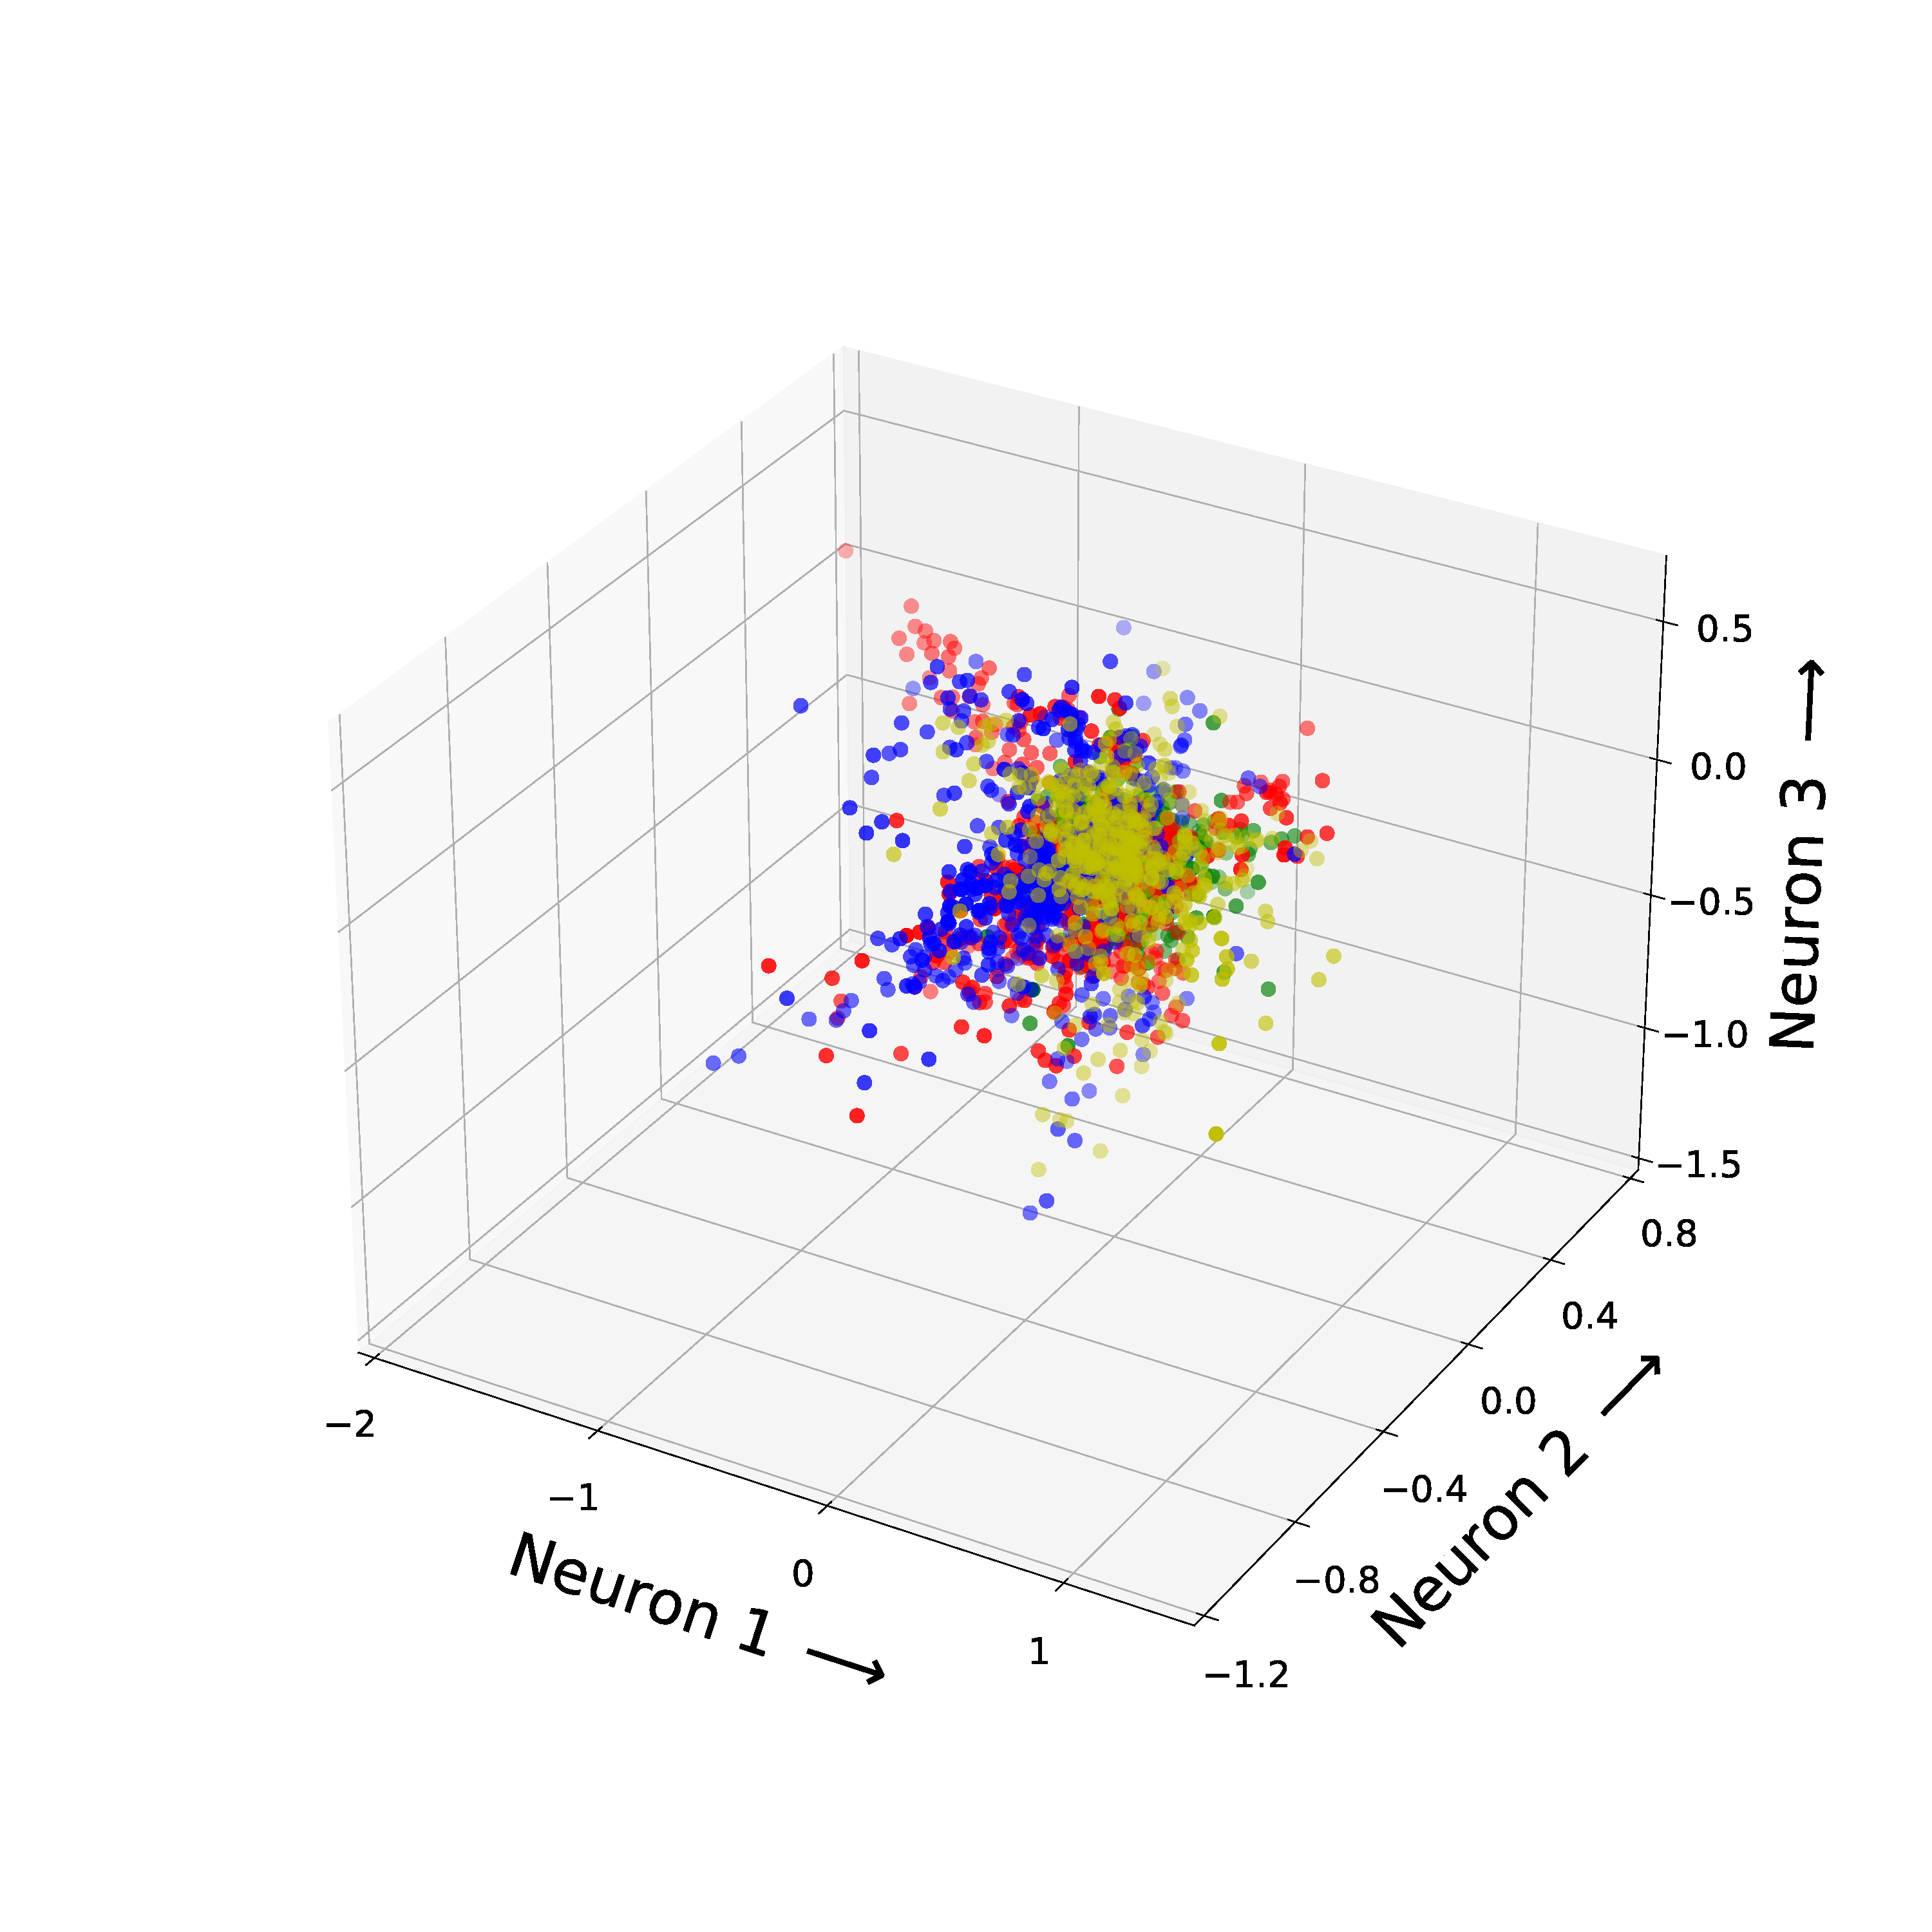
\includegraphics[width=.48\textwidth]{GAMMA_Influence_dummy_distribution/Dummy_distribution_0_GAMMA_0_001.pdf}
  \hspace{.4cm}
  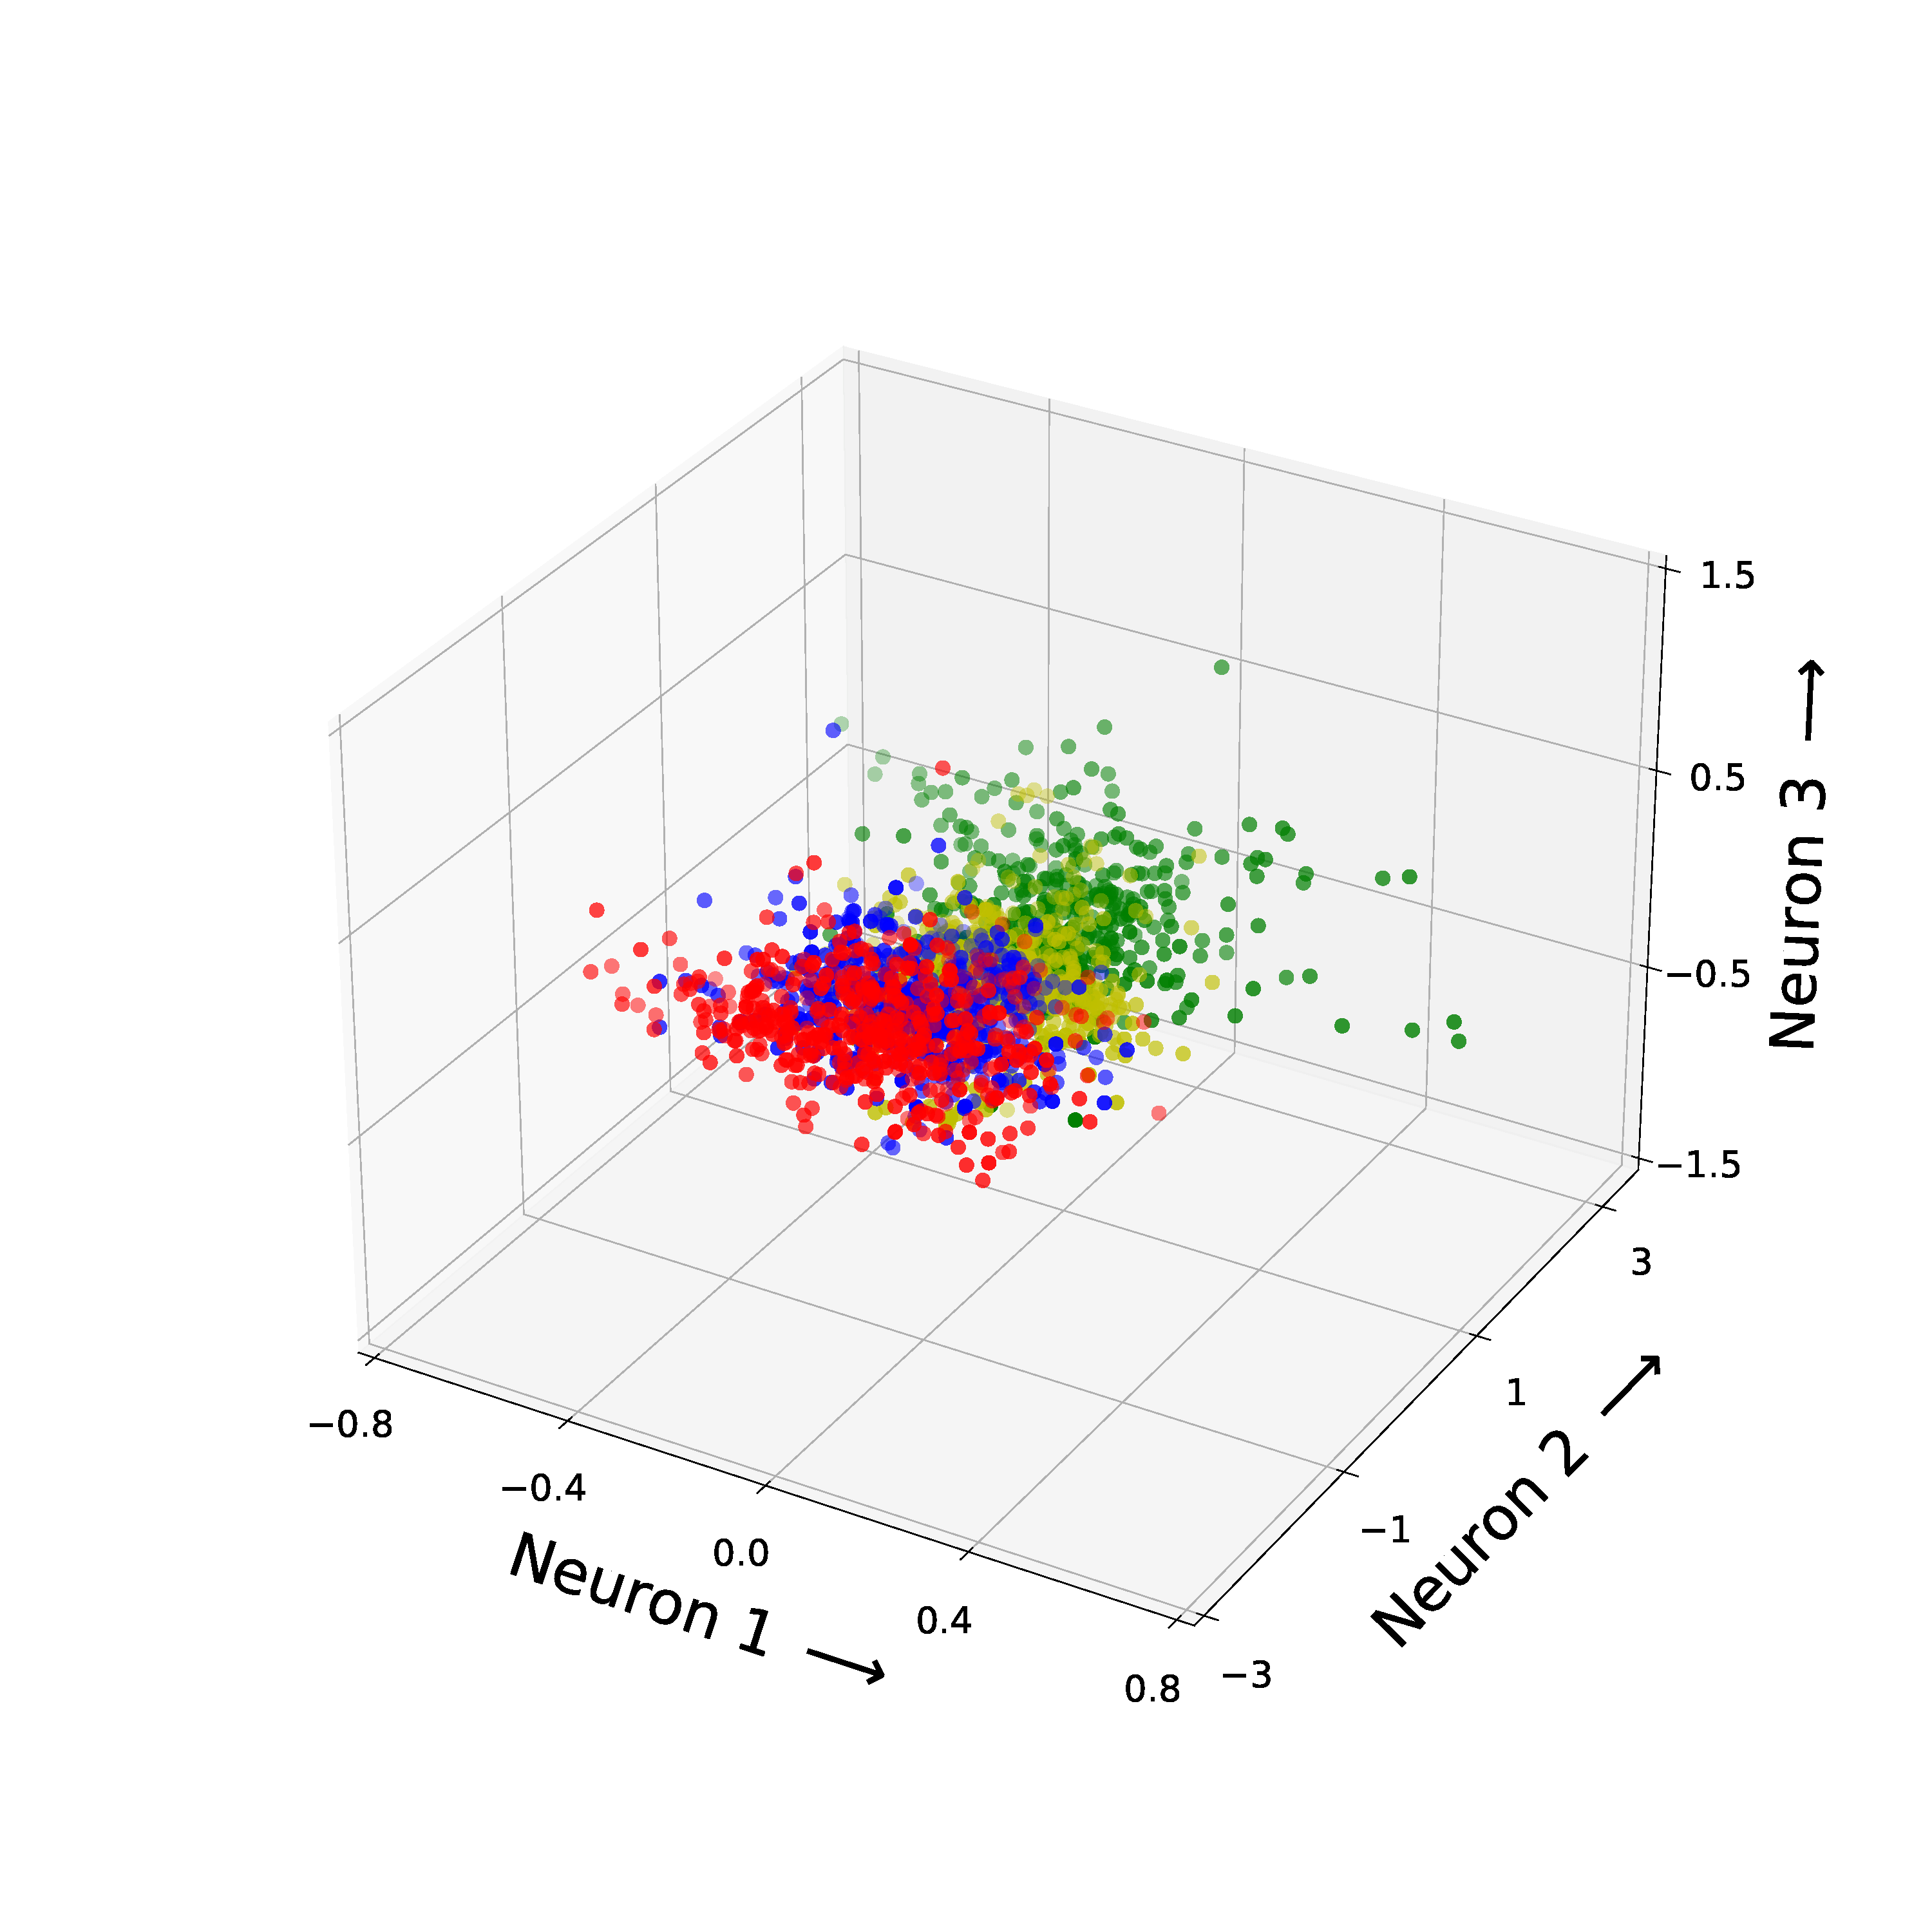
\includegraphics[width=.48\textwidth]{GAMMA_Influence_dummy_distribution/Dummy_distribution_8_GAMMA_0_001.pdf}

  \vspace{.1cm}

  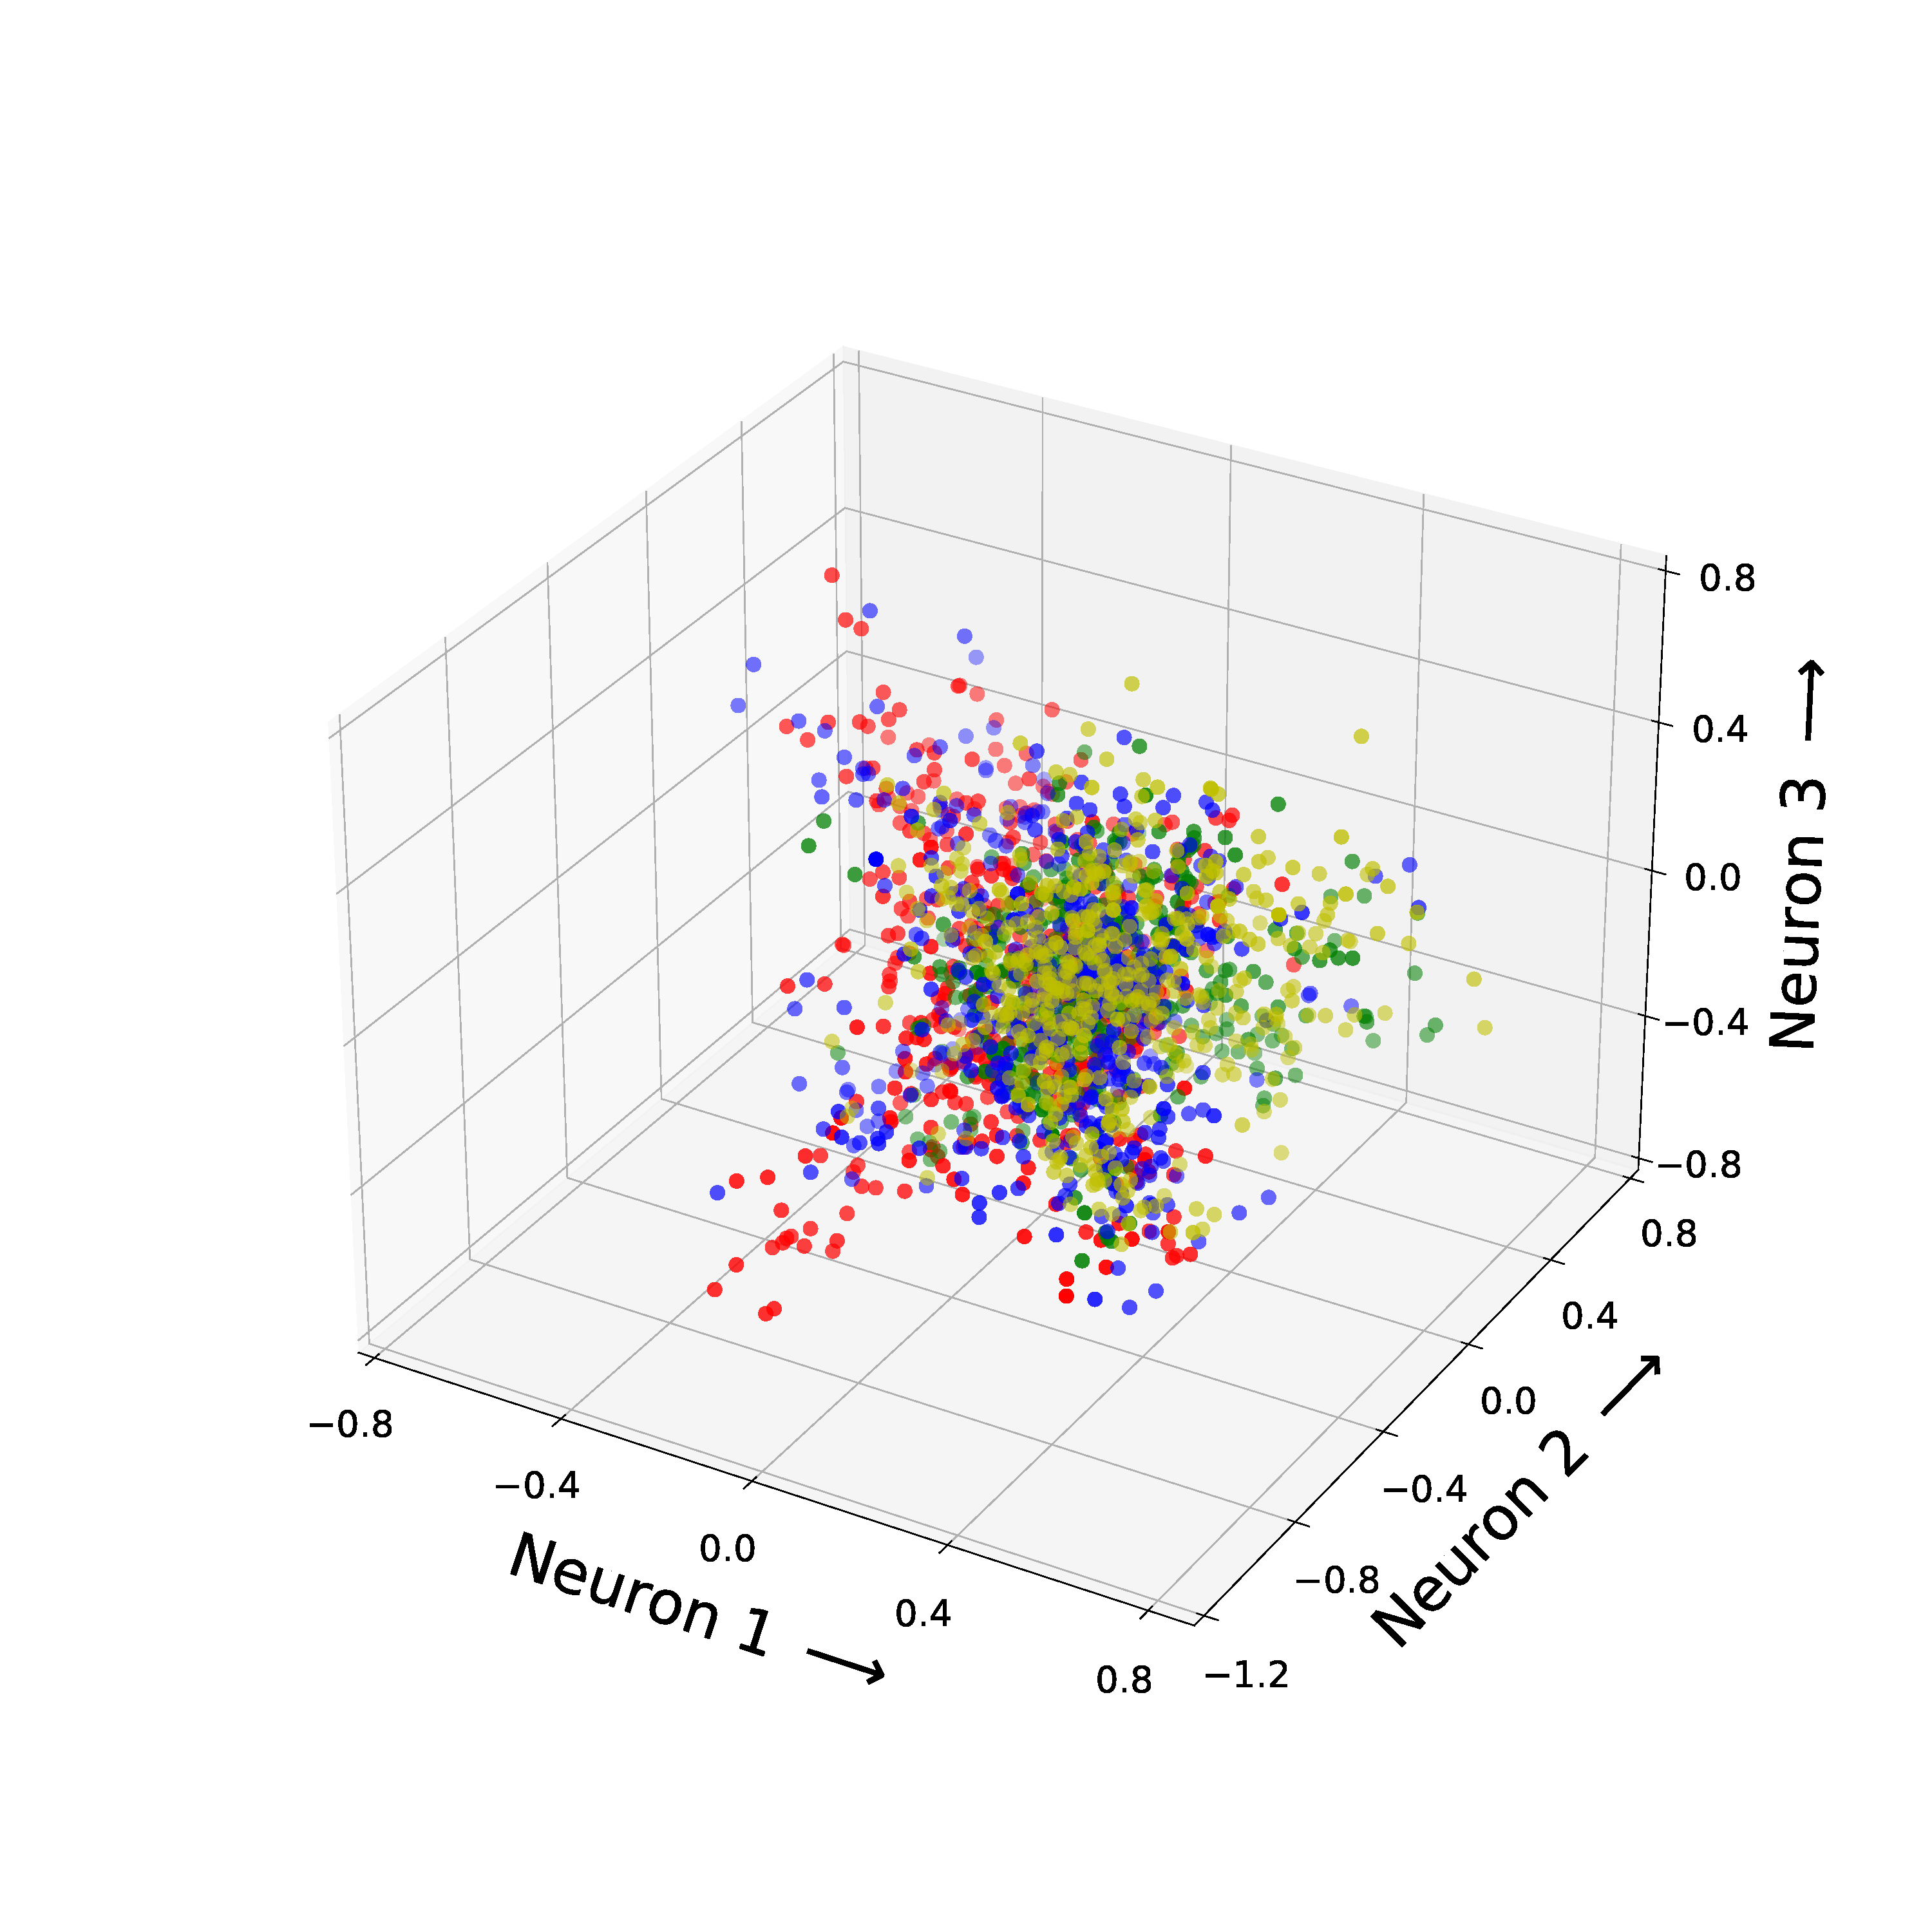
\includegraphics[width=.48\textwidth]{GAMMA_Influence_dummy_distribution/Dummy_distribution_0_GAMMA_0_1.pdf}
  \hspace{.4cm}
  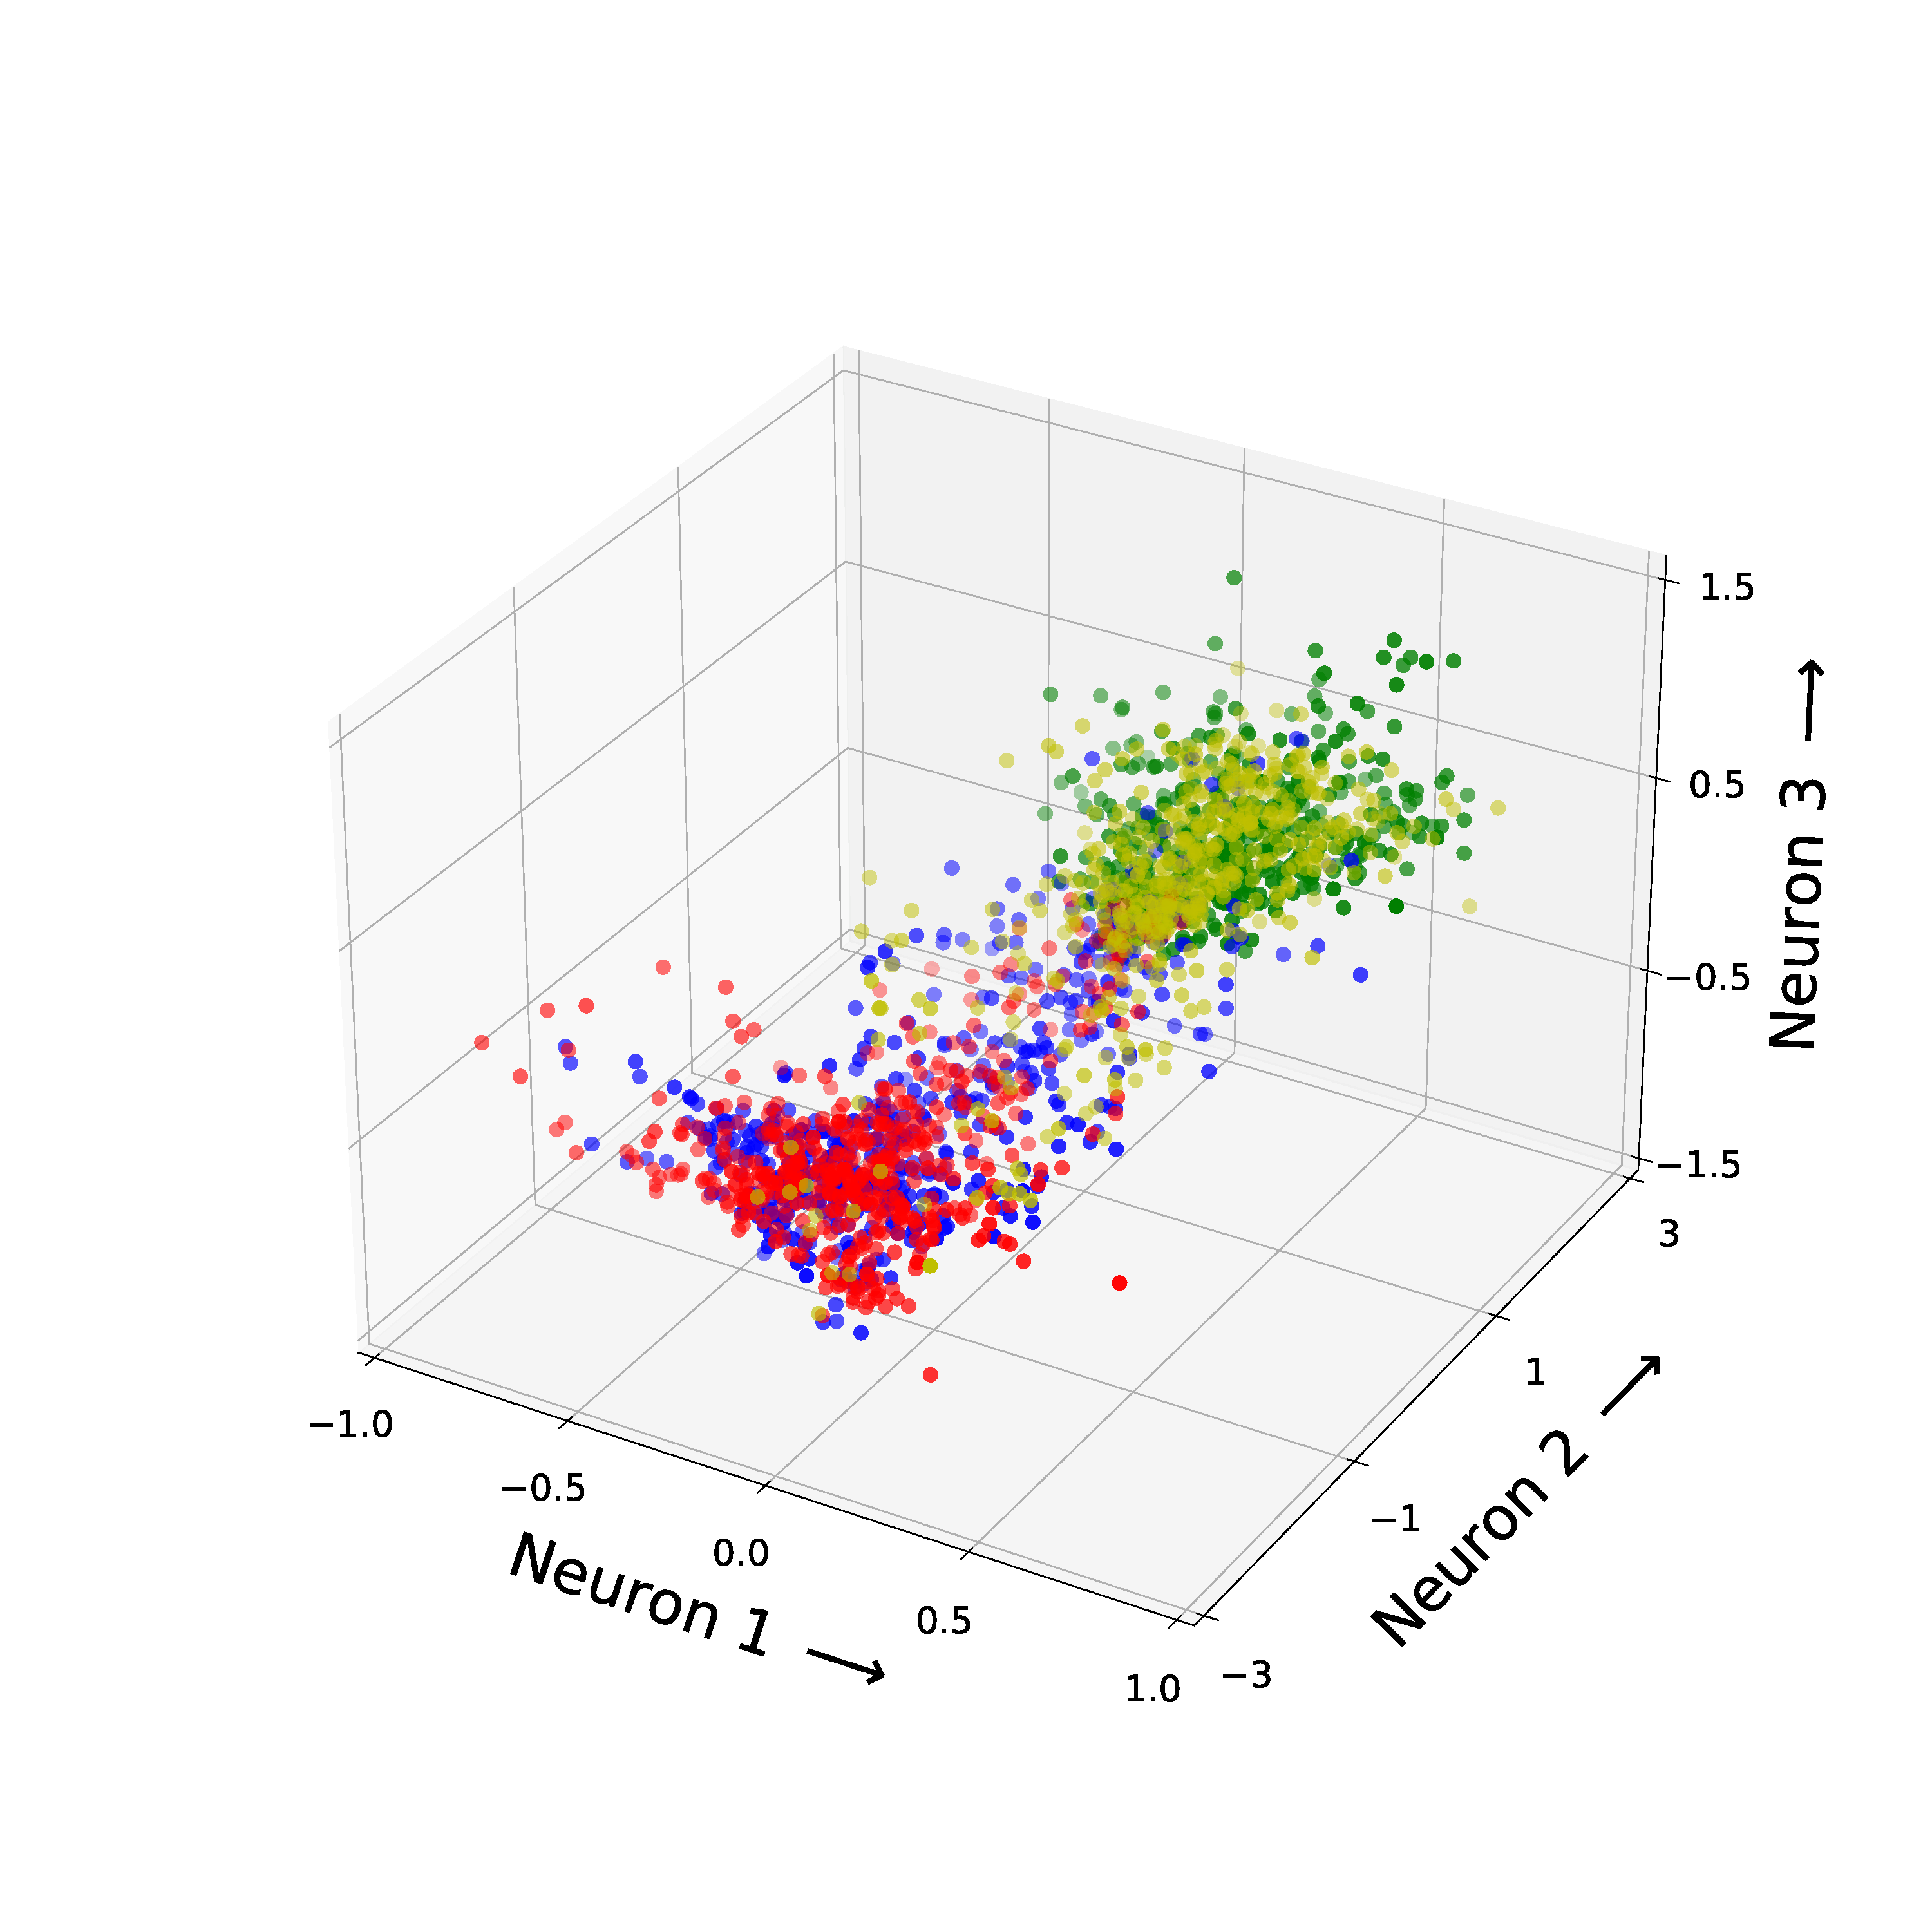
\includegraphics[width=.48\textwidth]{GAMMA_Influence_dummy_distribution/Dummy_distribution_8_GAMMA_0_1.pdf}

  \vspace{.1cm}

  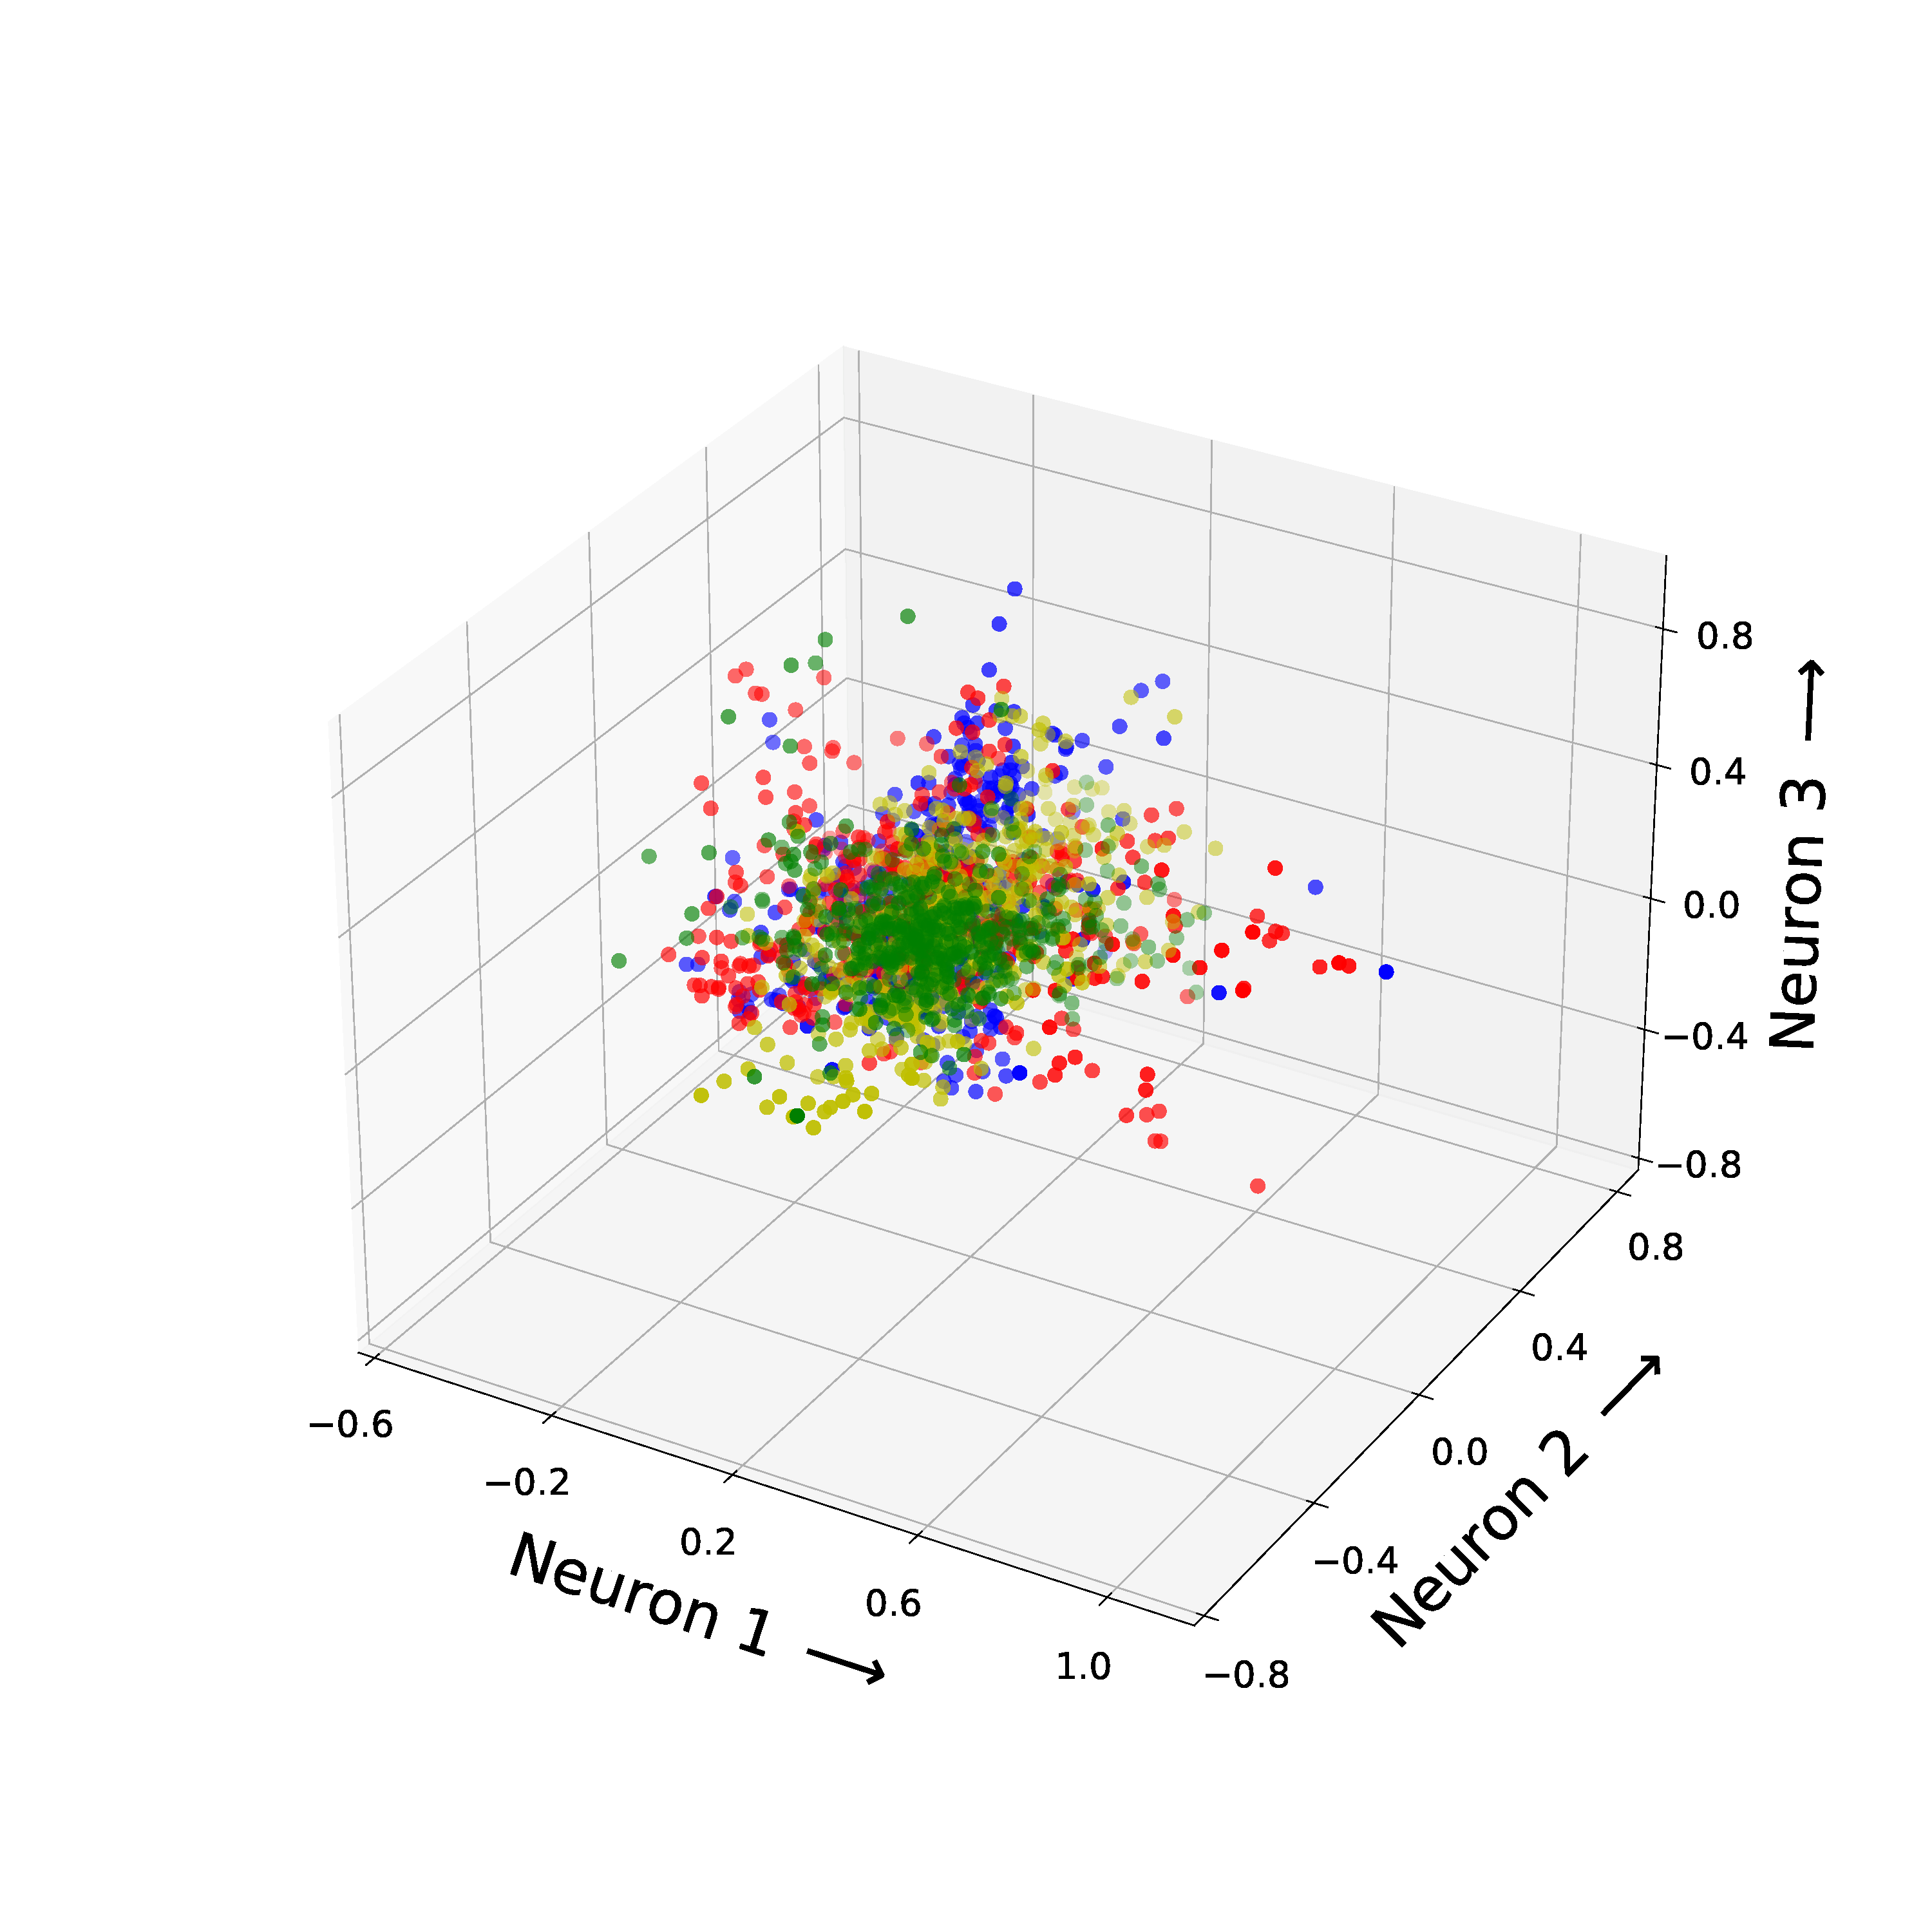
\includegraphics[width=.48\textwidth]{GAMMA_Influence_dummy_distribution/Dummy_distribution_0_GAMMA_20.pdf}
  \hspace{.4cm}
  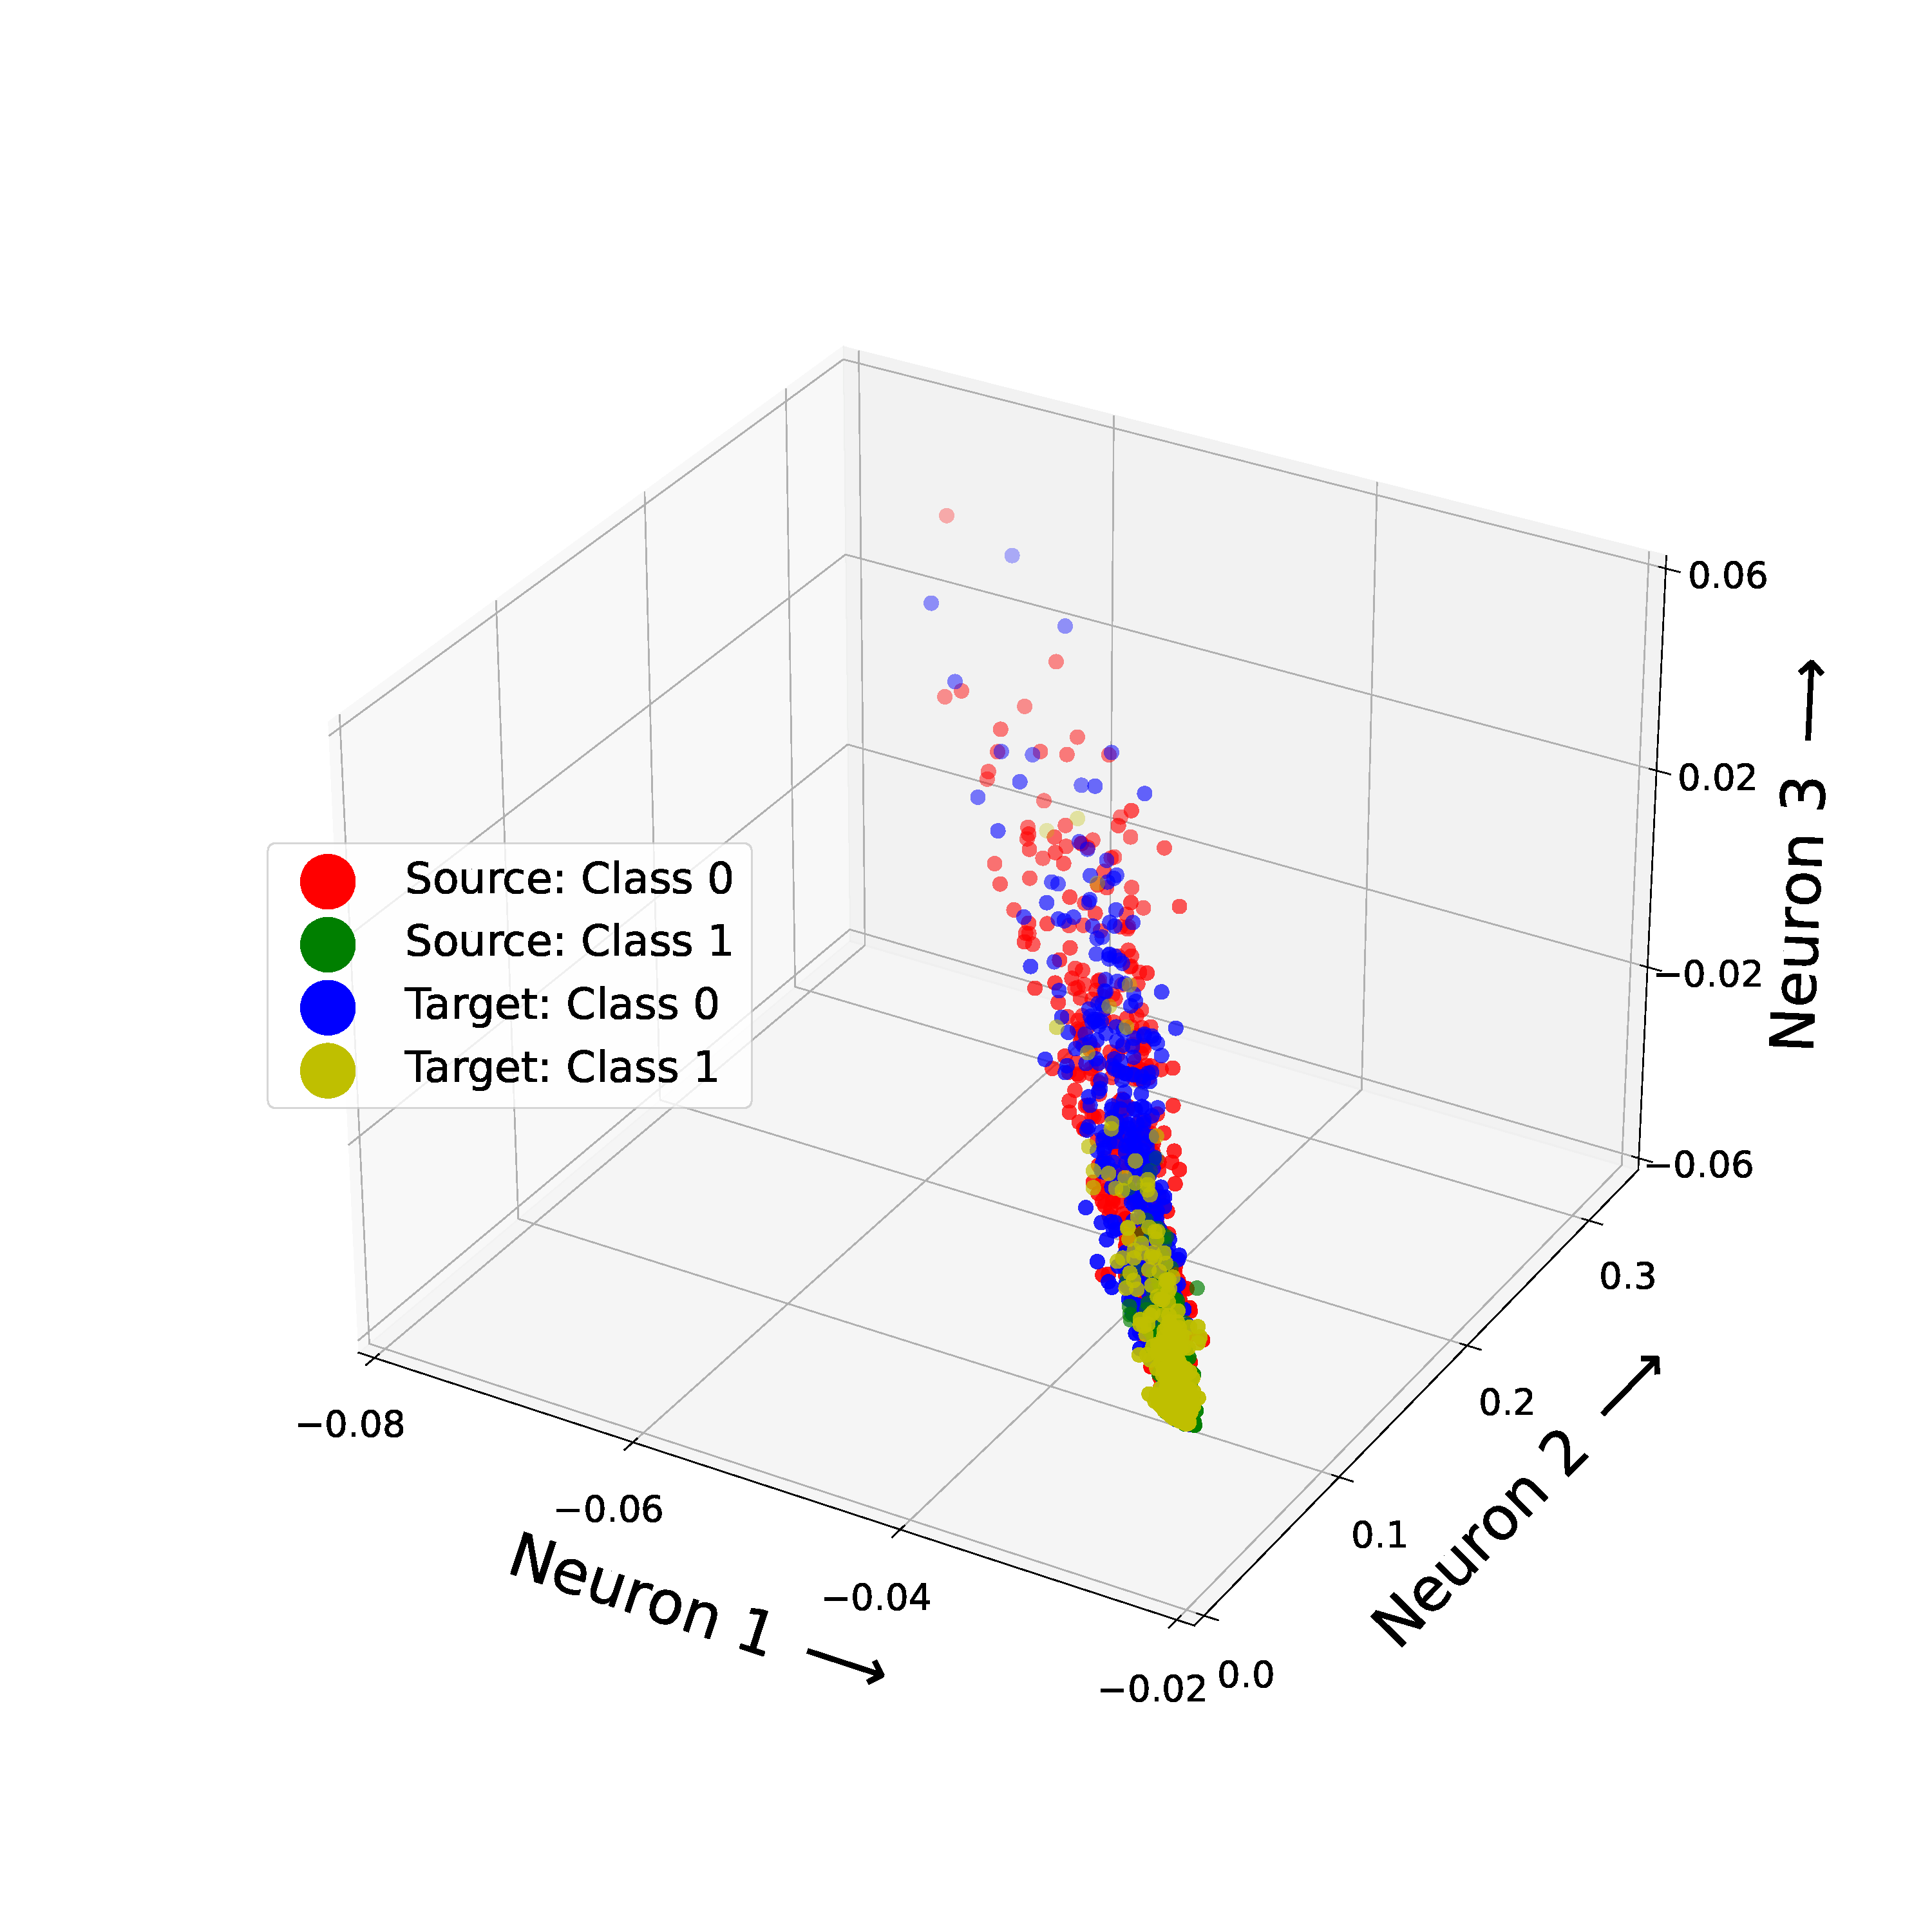
\includegraphics[width=.48\textwidth]{GAMMA_Influence_dummy_distribution/Dummy_distribution_8_GAMMA_20.pdf}
 

  \caption{Data distribution: Influence of GAMMA on Training, GAMMA = 0.05 (top), GAMMA = 0,4 (middle), GAMMA = 20 (bottom), Epoch = 0 (left) , Epoch = 8 (right)}
  \label{fig:point_cloud_mmd}
\end{figure}


\begin{figure}[H]
  \centering
  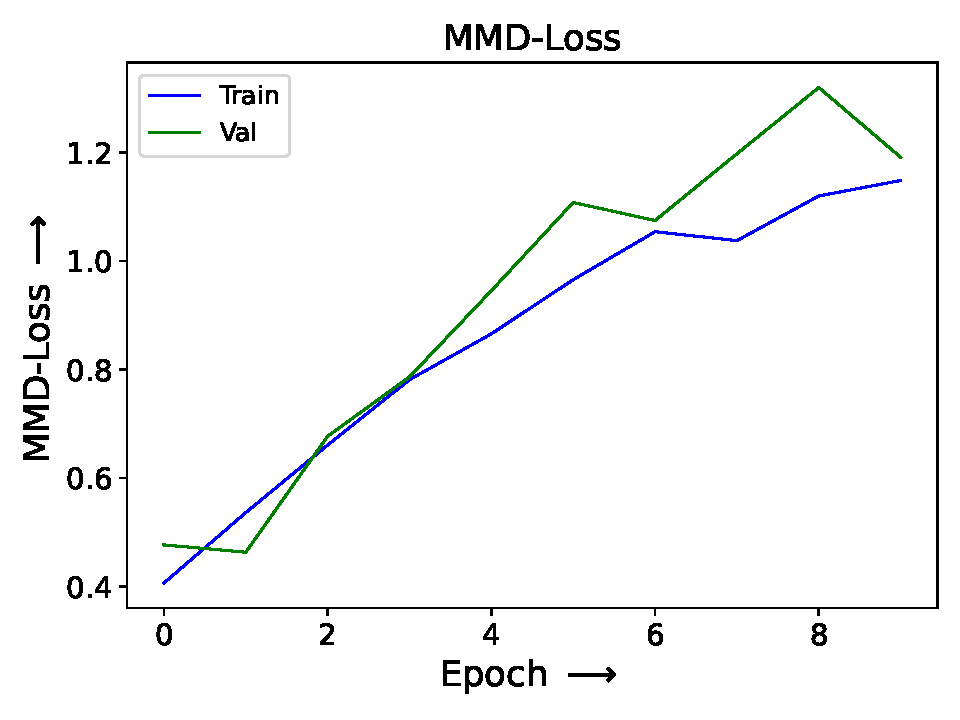
\includegraphics[width=.47\textwidth]{GAMMA_Influence_dummy_curve/MMD_Loss_GAMMA_0_001.pdf}
  \hspace{.3cm}
  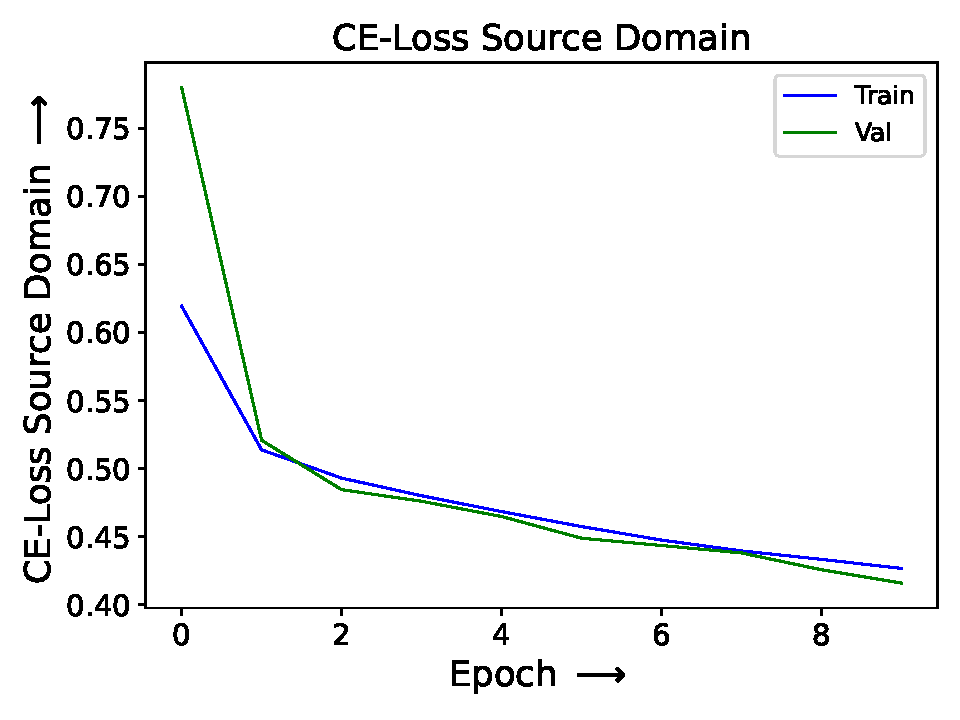
\includegraphics[width=.47\textwidth]{GAMMA_Influence_dummy_curve/CE_Loss_Source_Domain_GAMMA_0_001.pdf}

  \vspace{.1cm}

  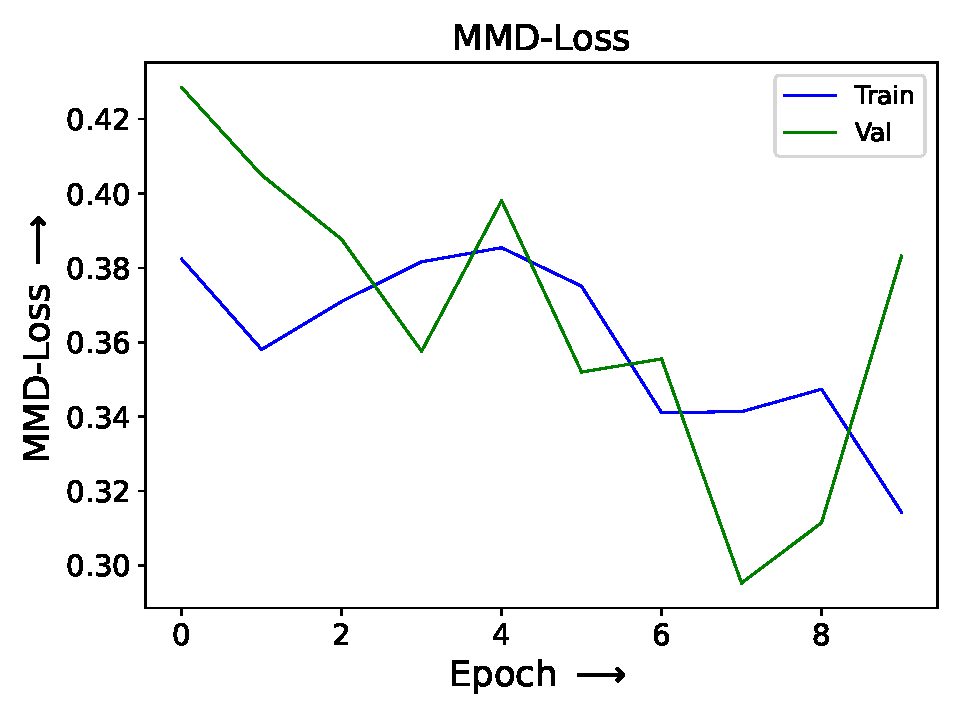
\includegraphics[width=.47\textwidth]{GAMMA_Influence_dummy_curve/MMD_Loss_GAMMA_0_1.pdf}
  \hspace{.3cm}
  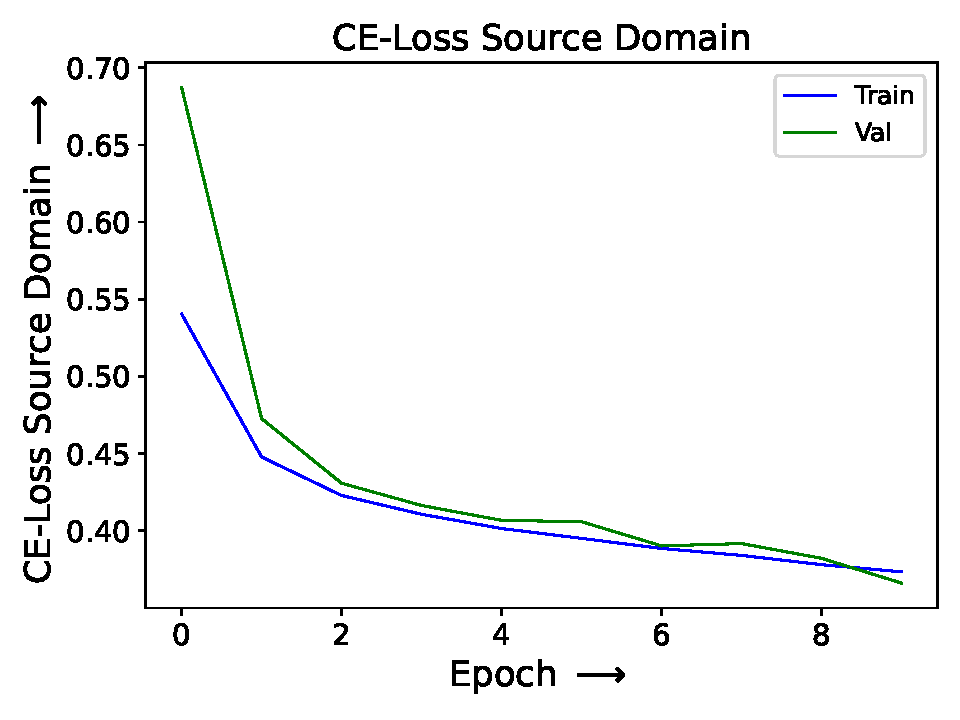
\includegraphics[width=.47\textwidth]{GAMMA_Influence_dummy_curve/CE_Loss_Source_Domain_GAMMA_0_1.pdf}

  \vspace{.1cm}

  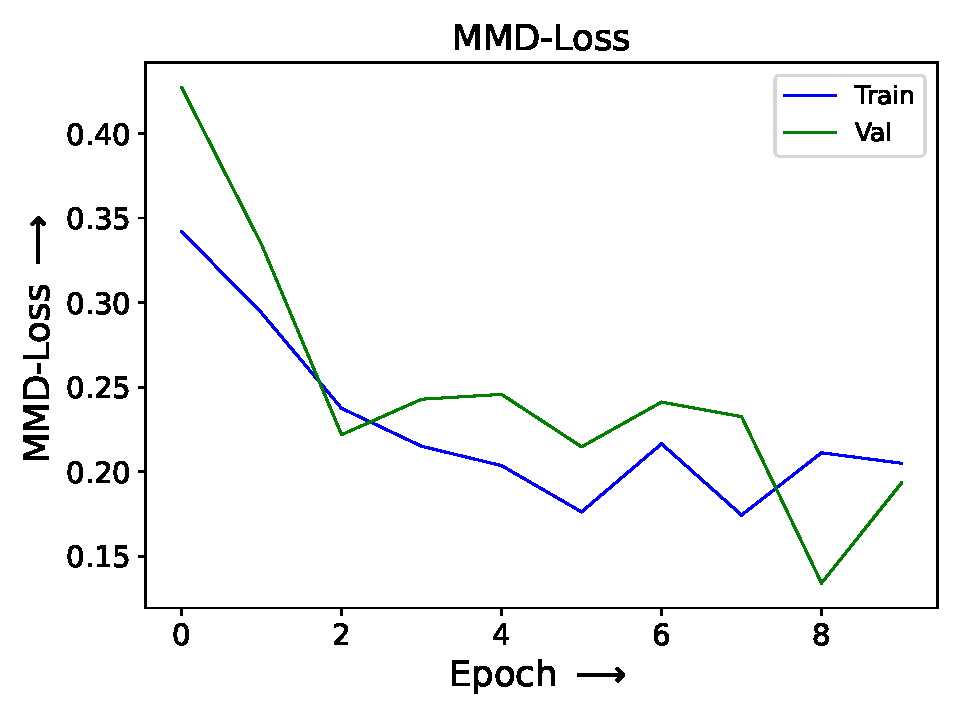
\includegraphics[width=.47\textwidth]{GAMMA_Influence_dummy_curve/MMD_Loss_GAMMA_20.pdf}
  \hspace{.1cm}
  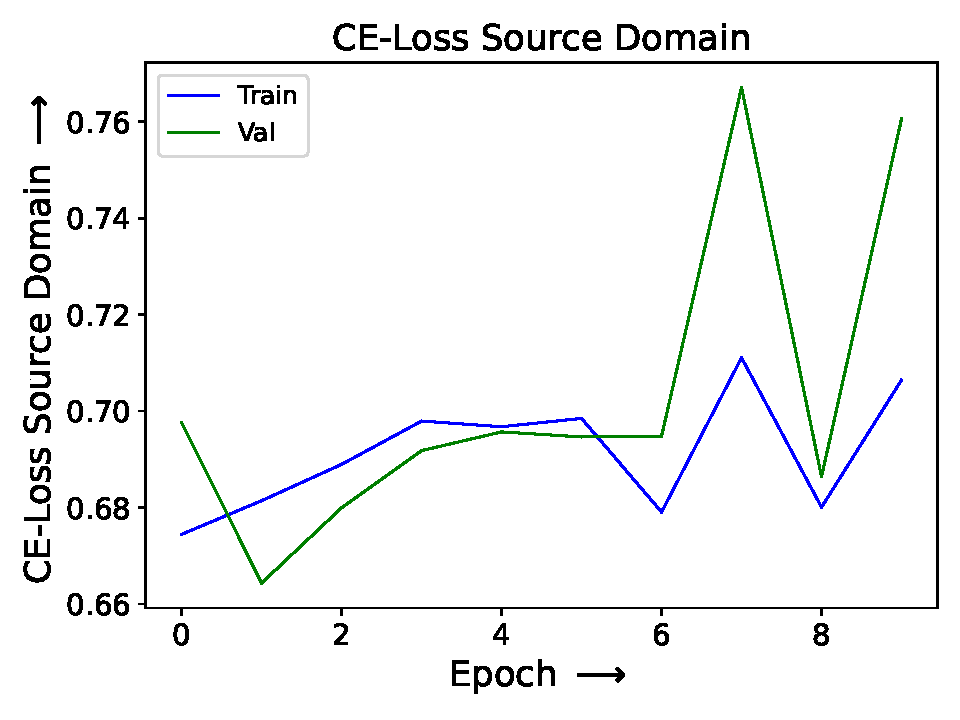
\includegraphics[width=.47\textwidth]{GAMMA_Influence_dummy_curve/CE_Loss_Source_Domain_GAMMA_20.pdf}

  \caption{MMD- and source CE-loss: Influence of GAMMA on Training: GAMMA = 0.001 (top), GAMMA = 0.1 (middle), GAMMA = 20 (bottom), Epoch 0 (left), Epoch 8 (right)}
  \label{fig:learning_curves_influence_mmd_feature_extractor}
\end{figure}

\subsection{Domain Adaptation Performance of a Labeled MMD-loss} \label{sec:Differences of labeled and unlabeled MMD loss}

In the unlabeled MMD-loss, the target labels are unknown. Therefore, the intra- and inter-class distance between source and target samples are minimized equally. Like mentioned earlier, this increases the compactness but reduces the class separability in both domains. In the literature some approaches, like the one proposed by Pandhare et al. \cite{Pandhare2021}, extend the unlabeled MMD-based model training with a distance-based optimization, which includes target labels. Usually those approaches restrict the supervised training to the source domain. In this section a novel labeled MMD-loss is presented, which includes target labels but restricts the supervised training to the source domain. The domain discrepancy between source and target samples of similar and different classes is optimized separately. The labeled MMD-loss minimizes the intra-class and maximizes the inter-class discrepancy between the domains. This separate consideration of class distances allows a simultaneous improvement of class separability and compactness. A weighted loss is applied which combines the source CE-loss, the intra-class and the inter-class MMD-loss. This approach expects additional hyperparameter, which need to be defined beforehand. The hyperparameters GAMMA\_Intra\_Class and GAMMA\_Inter\_Class are used to balance the training scope of maximizing the inter-class distance and minimizing the intra-class distance and source CE-loss:

\begin{equation}
\begin{split}
    \mbox{Total Loss} = & \mbox{GAMMA\_Intra\_Class}  \cdot \mbox{MMD\_Loss\_Intra\_Class} - \\
                              &\mbox{GAMMA\_Inter\_Class} \cdot \mbox{MMD\_Loss\_Inter\_Class} + \mbox{CE\_Loss}.
\end{split}
\end{equation}

The MMD-loss which includes the target labels is named "labeled MMD-loss" and otherwise "unlabeled MMD-loss". Again, fig. \ref{fig:point_cloud_labeled_unlabeled_mmd} visualizes the latent feature representation of the source and target samples in the FC2 layer. Throughout the training, the labeled MMD-loss is able to reduce the domain discrepancy while increasing the separability and compactness of the classes in both domains. In both domains the distance between the classes is increased by a lot. In the FC2 layer, the samples of the different classes are represented in a more distinct subsets. The subsets corresponding to the same classes overlap more across the different domains. These improvements, achieved by the labeled MMD-loss, simplify the classification problem. The labeled MMD-loss is interesting in a research aspect, since it reveals the deficits of the unlabeled MMD-loss. Due to the lack of target labels, the unlabeled MMD-loss must be tuned carefully and mostly improves the compactness and domain discrepancy and not so much the separability. When the effect of the unlabeled MMD-loss becomes too strong, the seperability between classes is destroyed and the optimization ends up in the trivial solution, in which the latent feature representation of all samples collapse to a point- or needle-like subspace. In the labeled MMD-loss the domain discrepancy between samples of the same class is reduced and otherwise increased. This guarantees a simultaneous improvement of the compactness and separability. Therefore, the GAMMA choice is less sensible in the training and the MMD-loss influence can be increased. The optimization is less prone to get stuck in the just described trivial solution. This is also the reason, why in this experiments GAMMA\_Inter\_Class and GAMMA\_Intra\_Class could both be chosen to be 30. Just 20\% of labeled target labels were used in labeled MMD-loss.

\begin{figure}[htp]
  \centering
  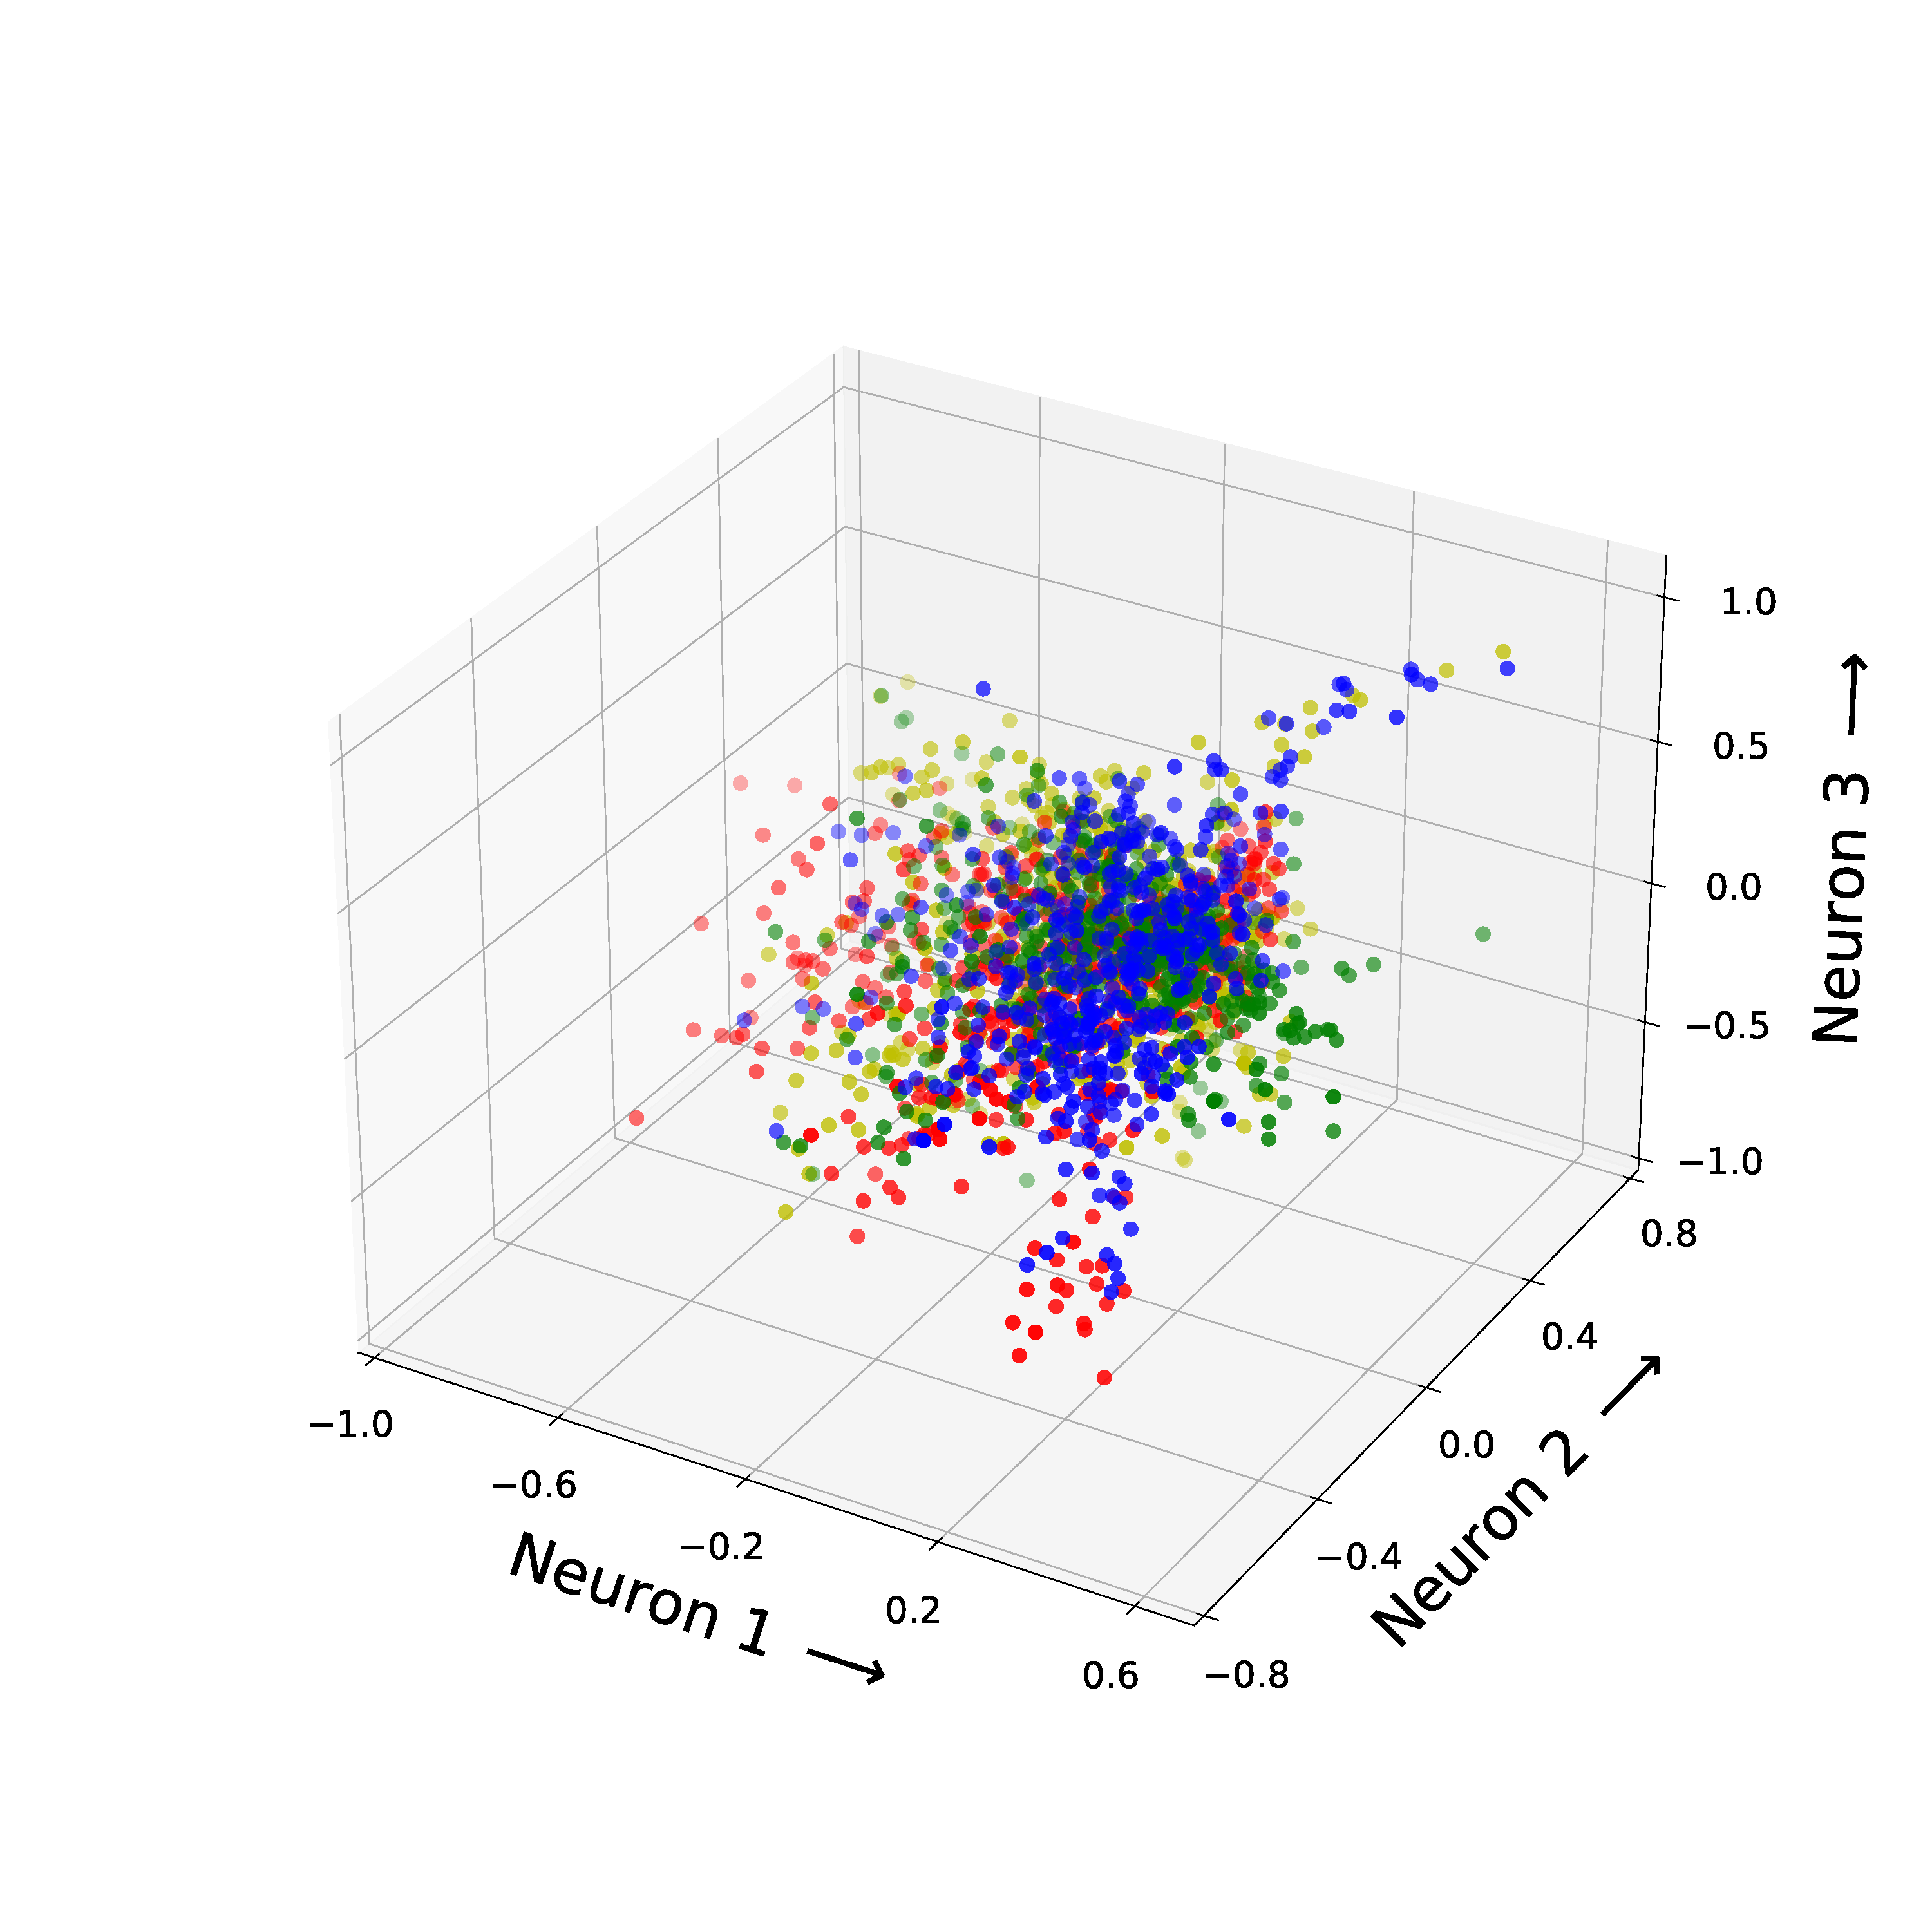
\includegraphics[width=.44\textwidth]{labeled_vs_unlabeled_point_cloud/data_distribution_labeled_mmd_0.pdf}
  \hspace{.4cm}
  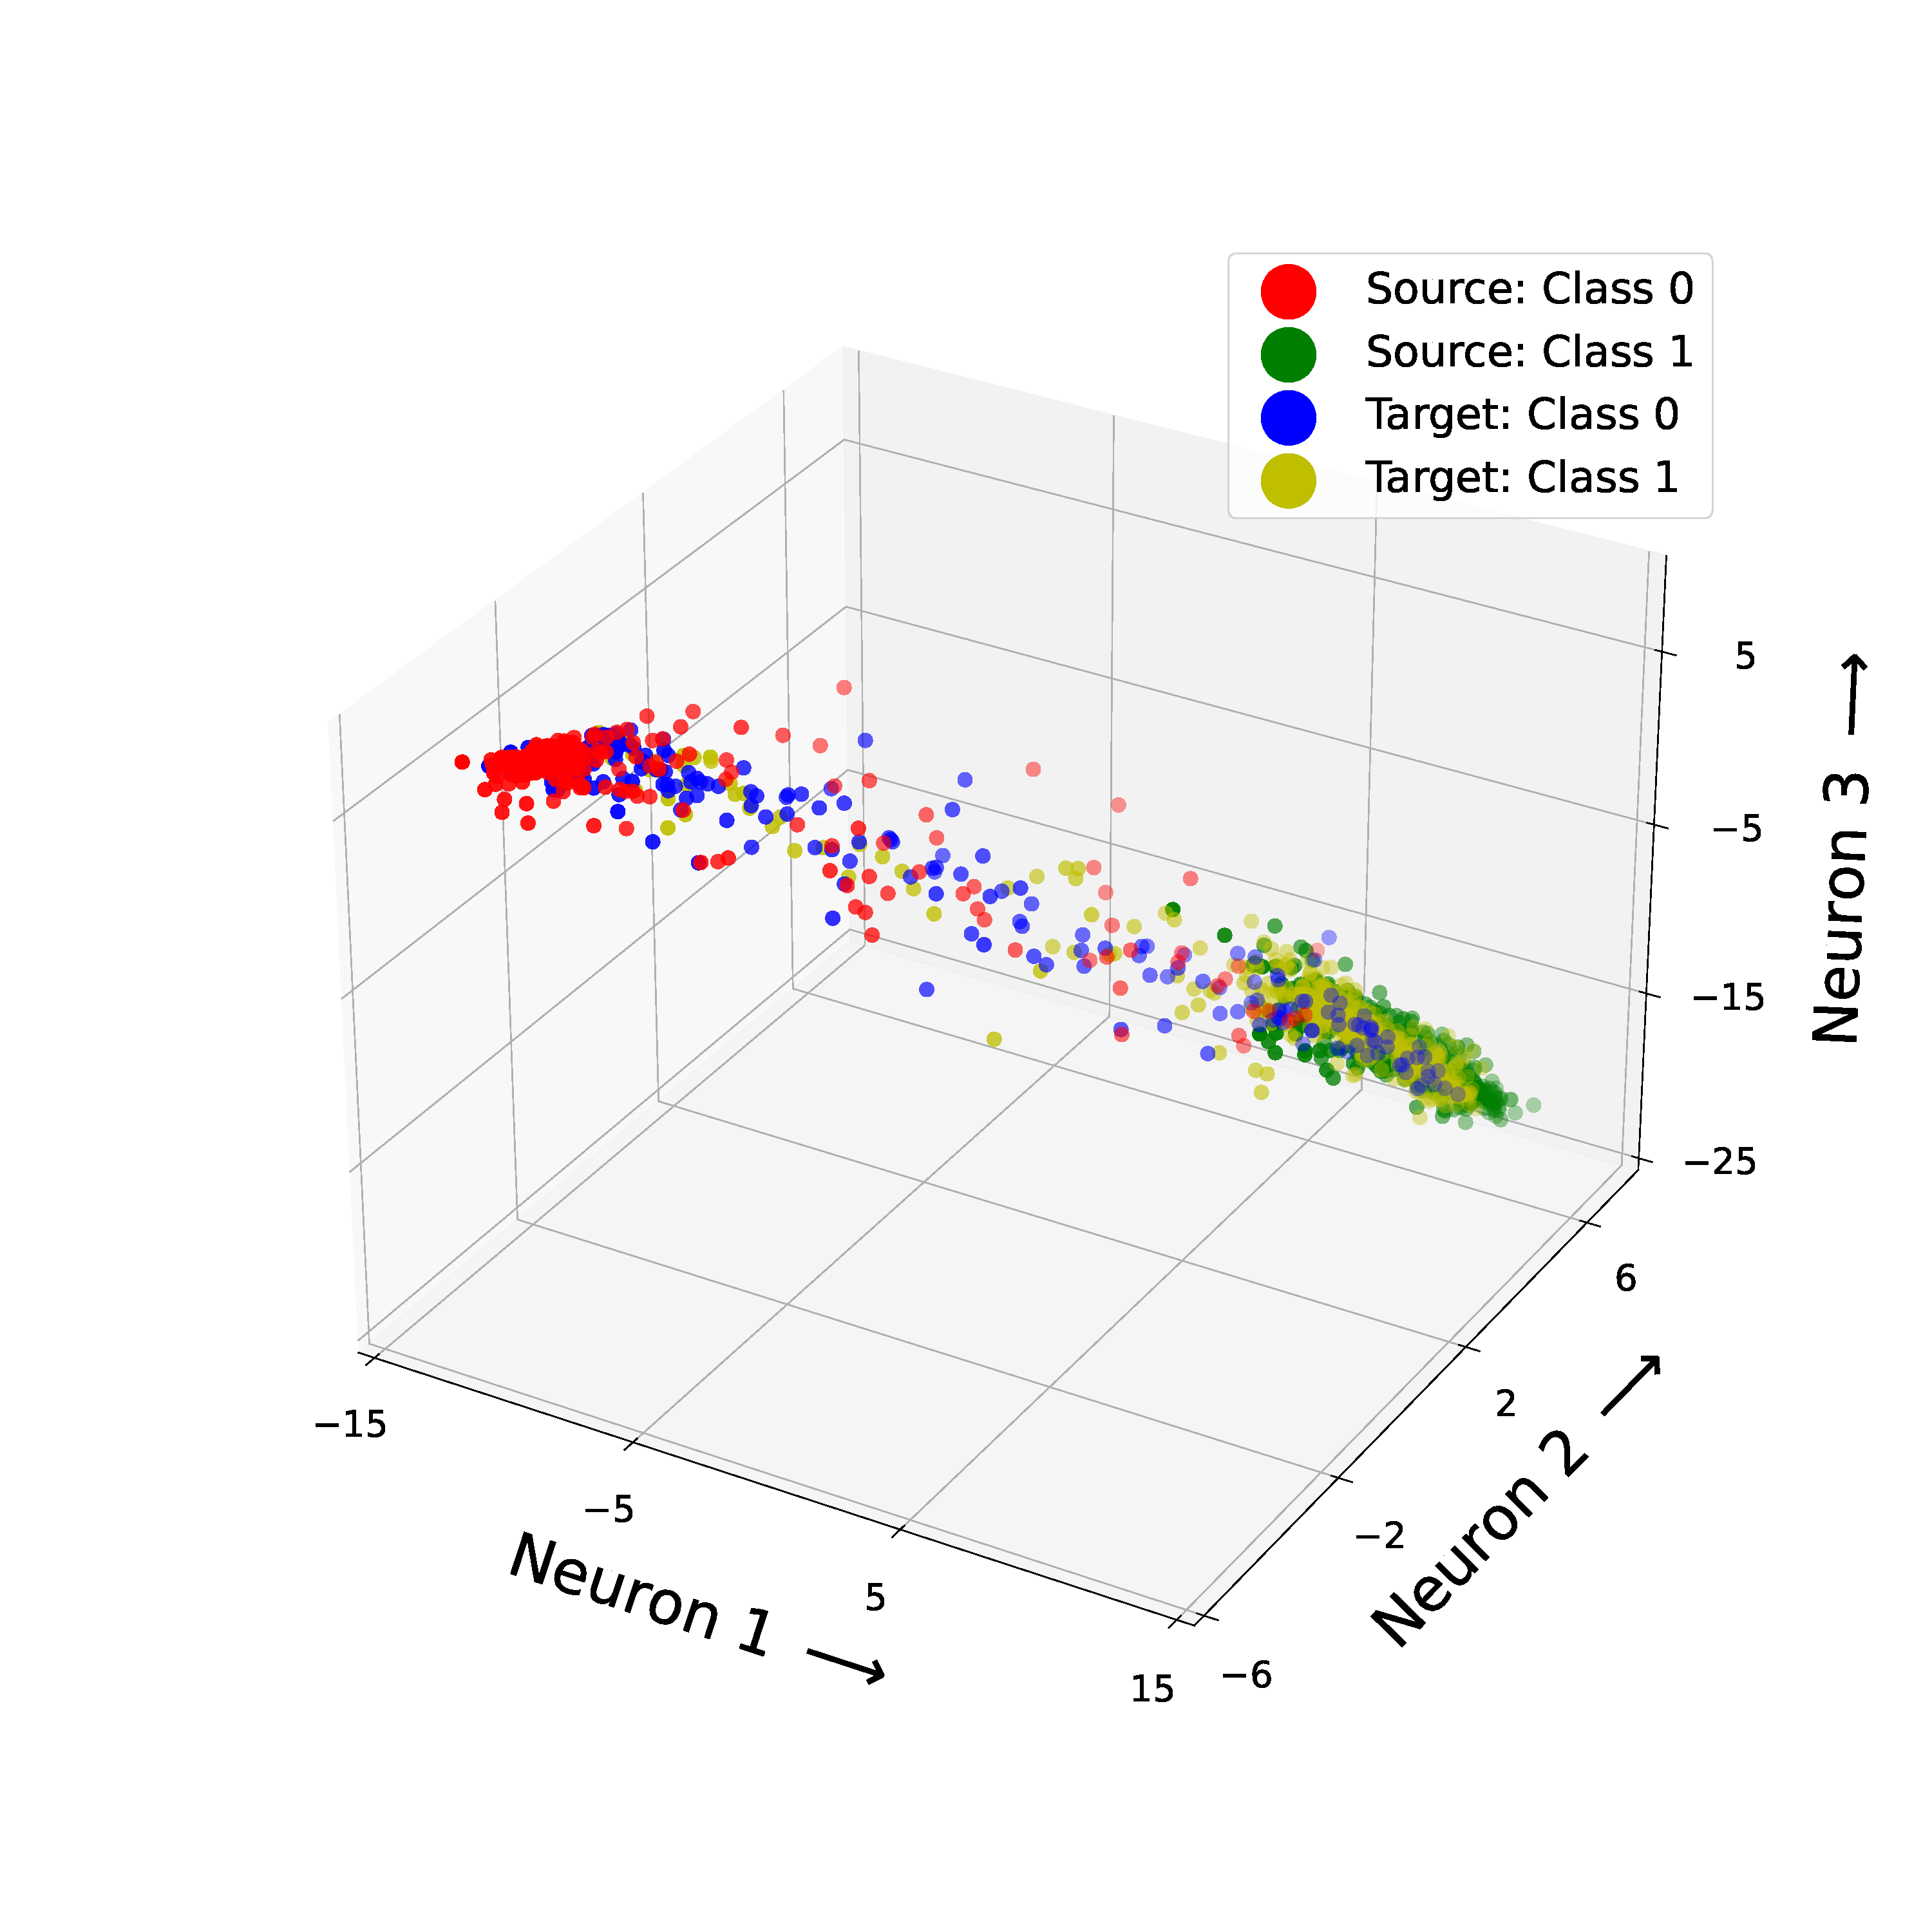
\includegraphics[width=.44\textwidth]{labeled_vs_unlabeled_point_cloud/data_distribution_labeled_mmd_8.pdf}

  \vspace{.1cm}

  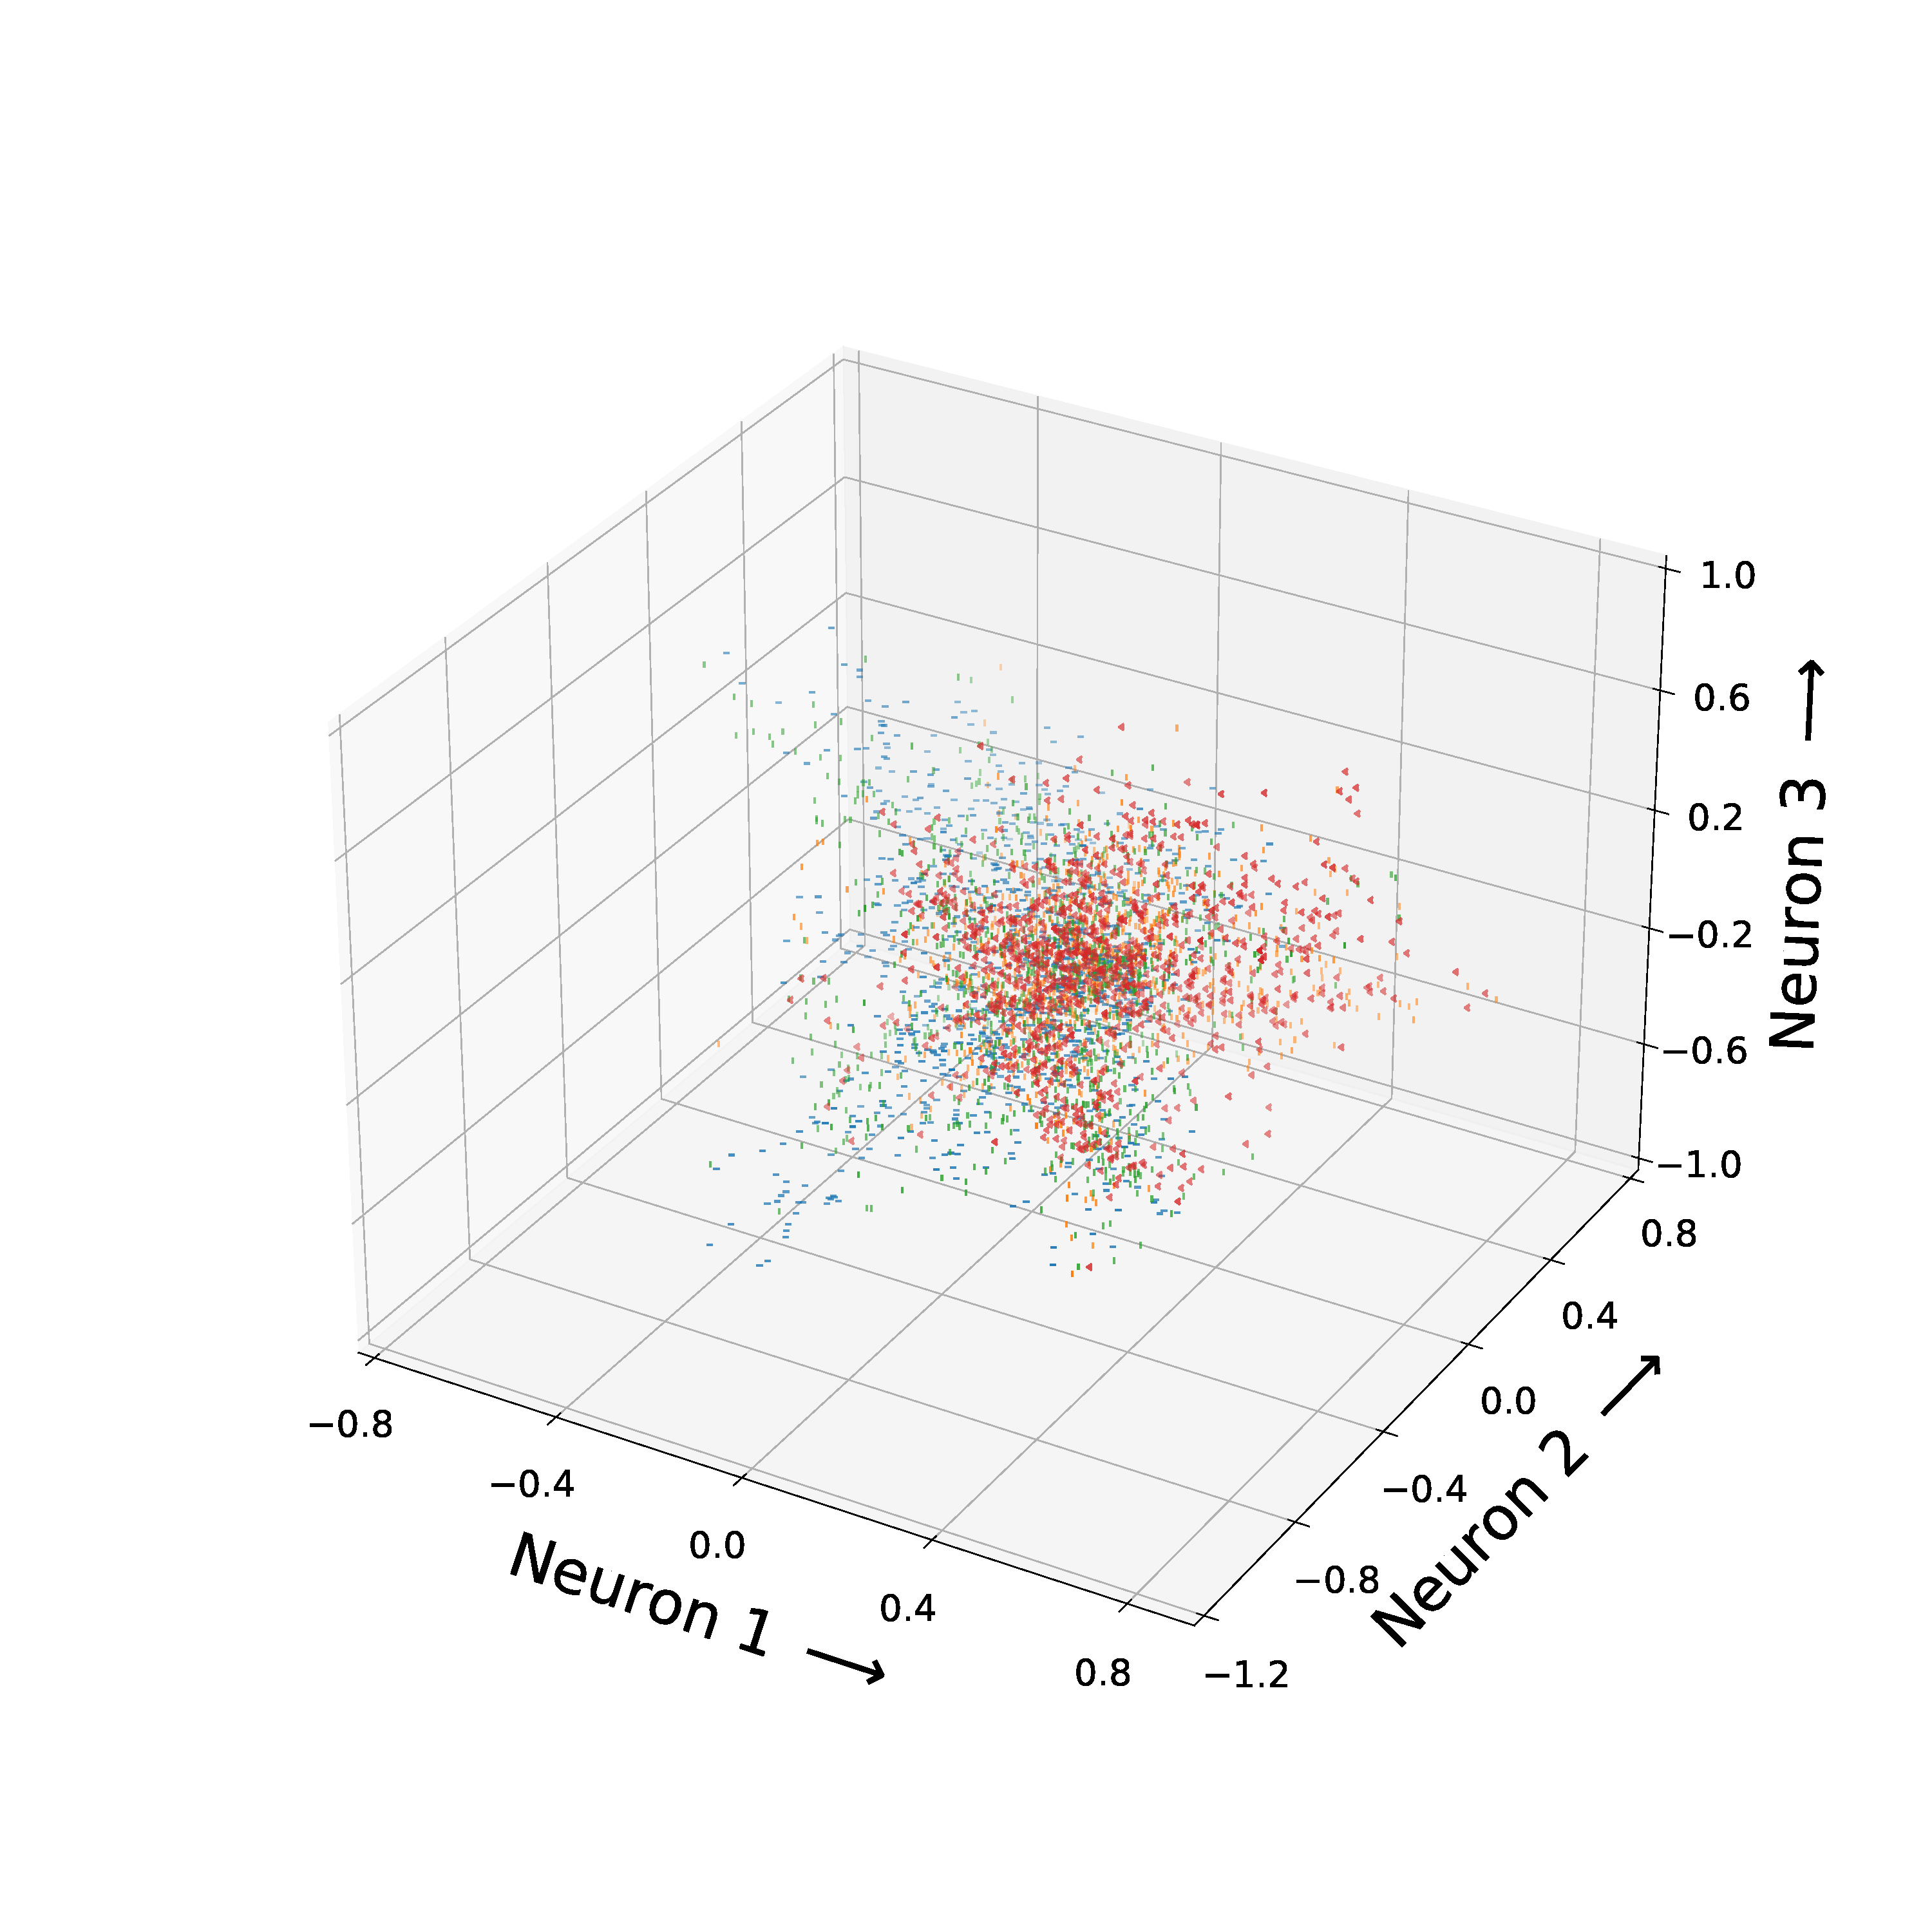
\includegraphics[width=.44\textwidth]{labeled_vs_unlabeled_point_cloud/data_distribution_regular_mmd_0.pdf}
  \hspace{.4cm}
  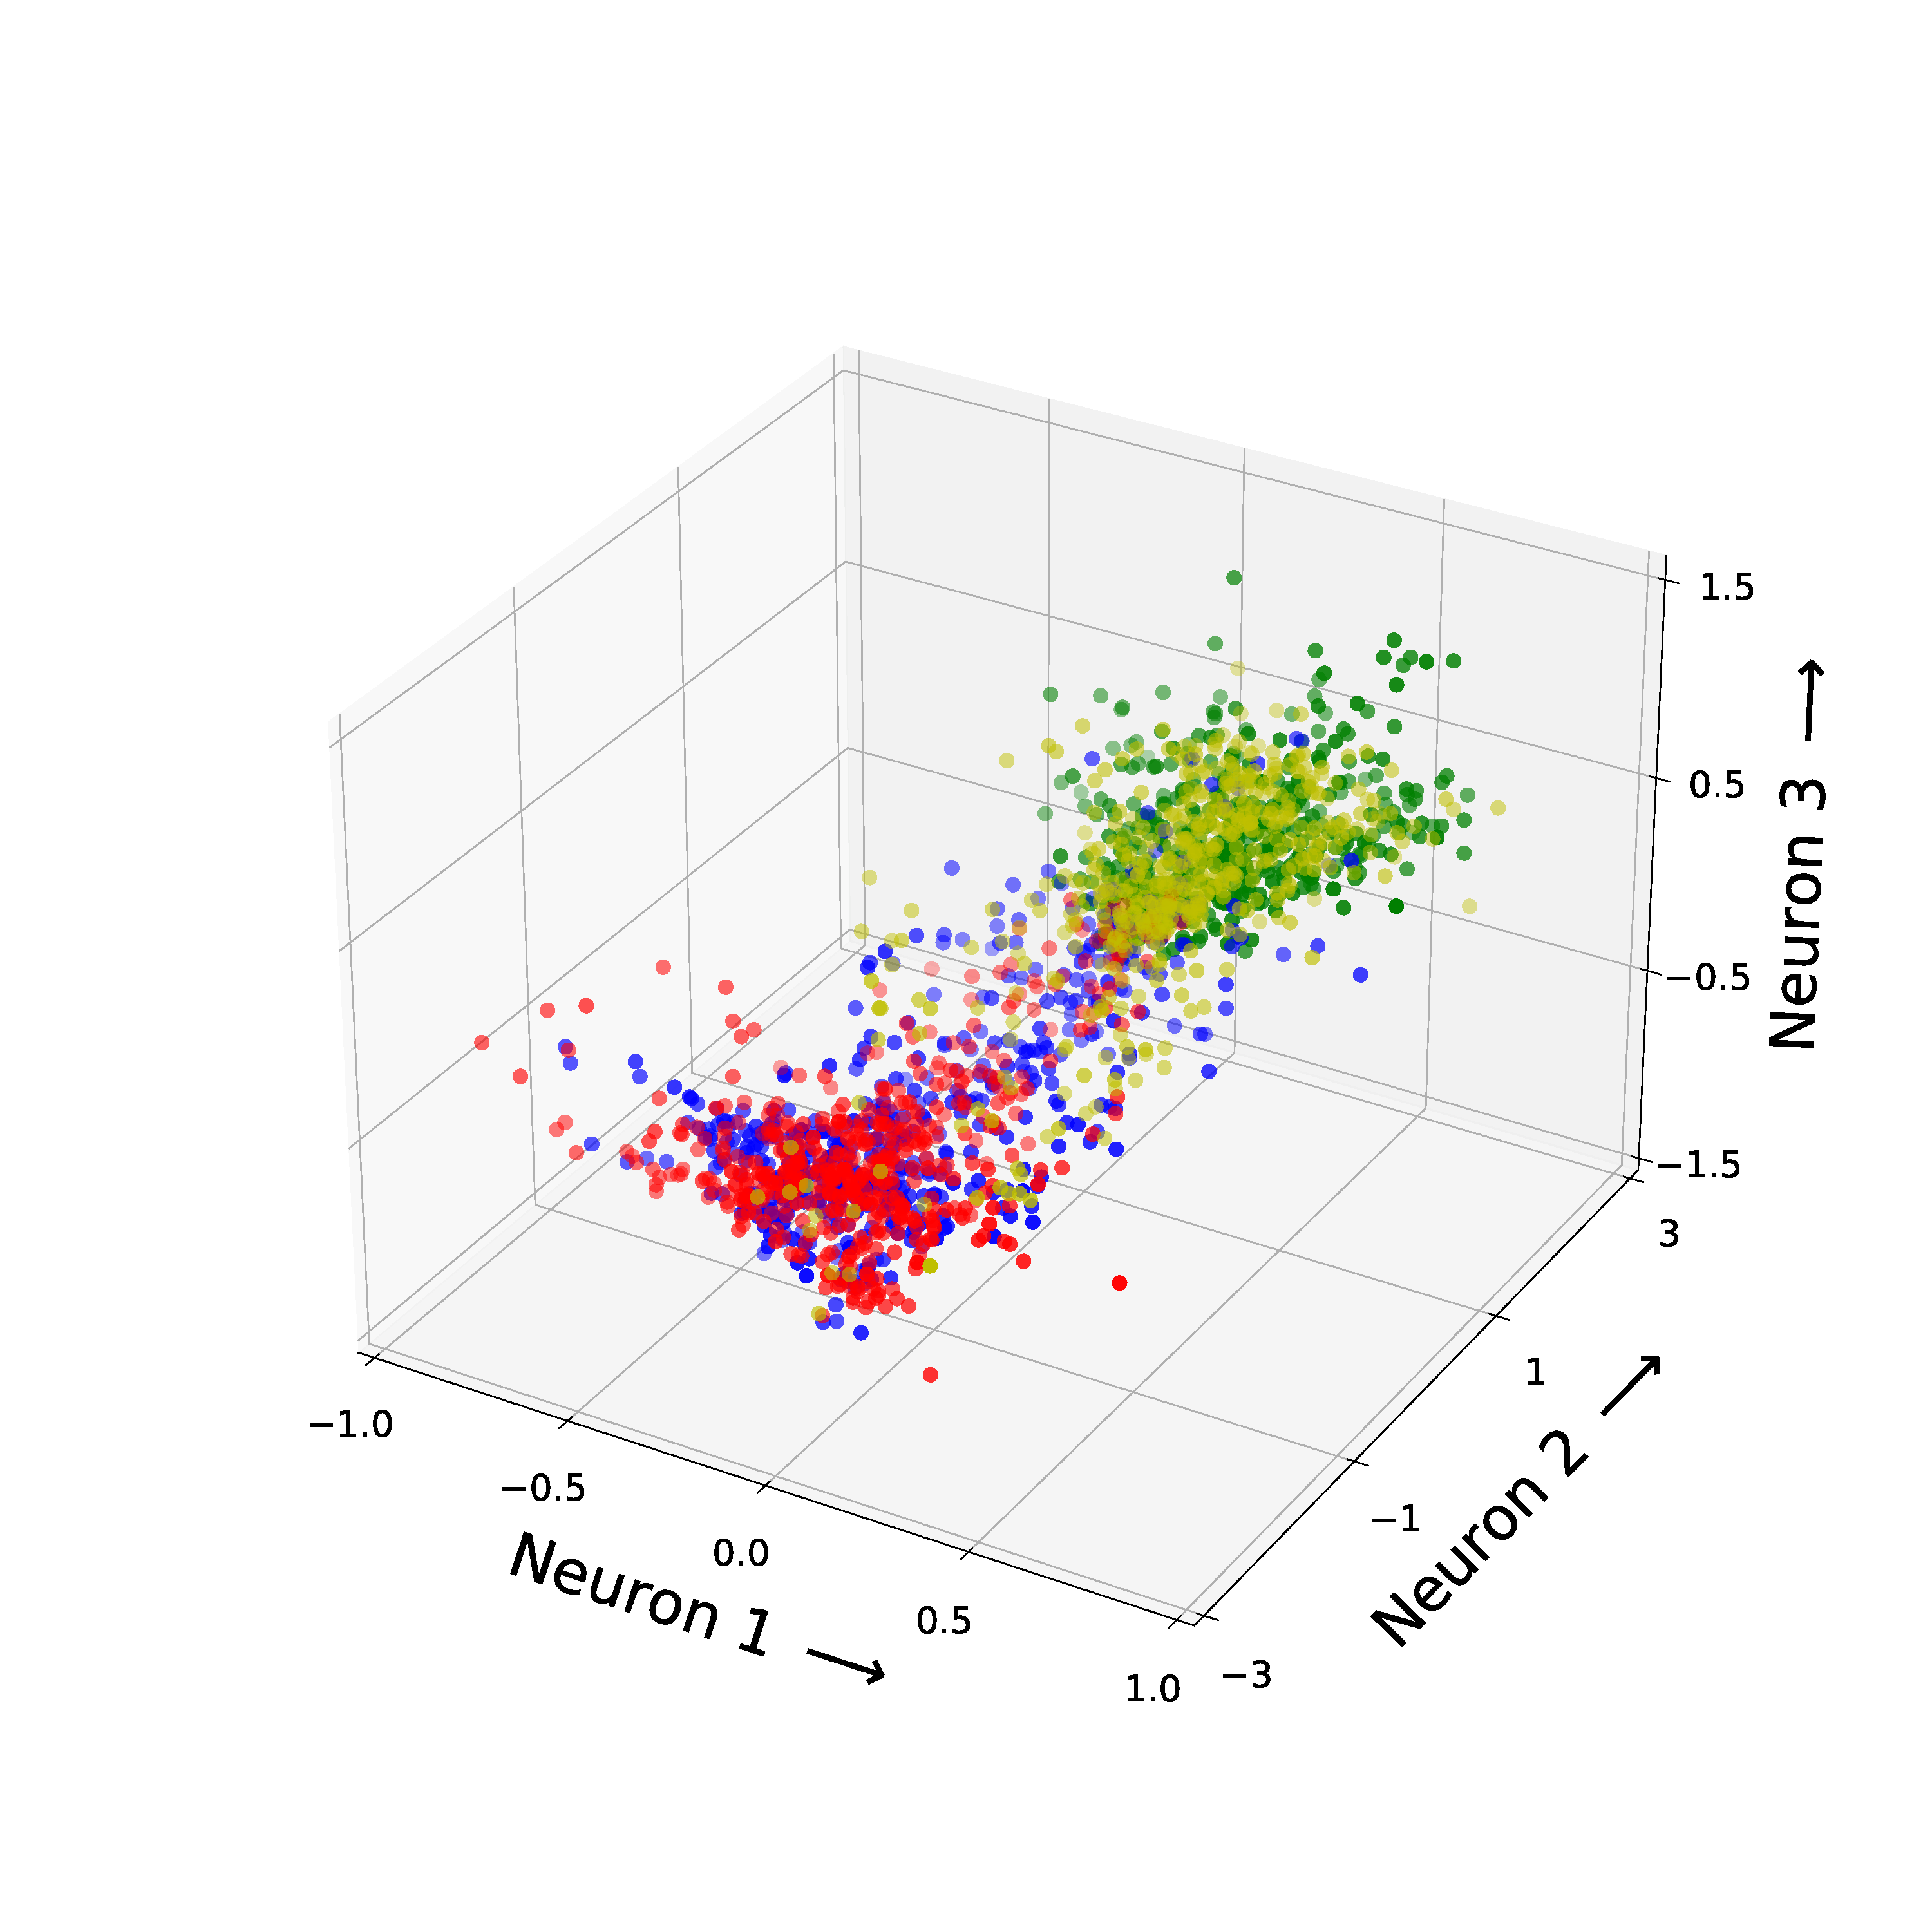
\includegraphics[width=.44\textwidth]{labeled_vs_unlabeled_point_cloud/data_distribution_regular_mmd_8.pdf}
  
  \caption{Data Distribution: Labeled MMD (top) vs. unlabeled MMD (bottom): Epoch 0 (left) vs. Epoch 8 (right)}
  \label{fig:point_cloud_labeled_unlabeled_mmd}
\end{figure}

\subsection{Influence of Latent Feature Space Choice on the Domain Adaptation Performance}
\label{cnn_mmd_dummy}

This section analyzes the influence of applying the MMD-loss in different latent feature maps of the feature extractor and classifier. Inspired by Aljundi et al. \cite{Aljundi2016}, especially the domain discrepancy reduction in the feature extractor layers is of great interest. Two MMD-based approaches were evaluated, which measure the domain discrepancy in different layers of the neural network. Table \ref{tab:MMD_layer_choice_dummy} specifies the applied MMD-loss types in more detail.

\begin {table}[H]
\centering

\begin{tabular}{llllllll}
  \toprule
  Model          & Conv1 & Conv2 & Conv3 & Flatten & FC1 & FC2 \\
  \midrule
  
 
\vspace{.5cm}

 \parbox[t]{0mm}{\multirow{1}{*}{\rotatebox[origin=c]{90}{\thead{FC \\ MMD}}}} & - & - & - & \checkmark & \checkmark & \checkmark\\
 
\vspace{.5cm}

 \parbox[t]{0mm}{\multirow{1}{*}{\rotatebox[origin=c]{90}{\thead{FULL \\ MMD}}}} & \checkmark & \checkmark & \checkmark & \checkmark & \checkmark & \checkmark\\

  \bottomrule
\end{tabular}

\caption {MMD layer choice of presented models} \label{tab:MMD_layer_choice_dummy} 
\end {table}

The development of the source and target accuracies as well as the source CE- and MMD-loss throughout the model training are visualized in fig. \ref{fig:accuracy_cnn_and_no_cnn_mmd} and fig. \ref{fig:loss_cnn_and_no_cnn_mmd}. When including the CNN feature maps in the MMD-loss, higher source and target accuracies are achieved. Besides that, the losses, as well as the accuracies, converge faster and smoother. As Li et al. \cite{li2020} mentioned, the domain shift is not tackled sufficiently when solely reducing the domain discrepancy only in the final layers of the neural network. When estimating the MMD- and CE-loss solely in the final layers, it seems like the two contradicting training goals work against each other. The model training seems to get stuck in local minima, which leads to instabilities. The corresponding fluctuations can be seen in the training curves. Anyhow, one has to remember calculating the FULL MMD-loss is quite expansive since the feature maps of the convolutional layers are complex and high-dimensional.

\begin{figure}[htp]
  \centering
  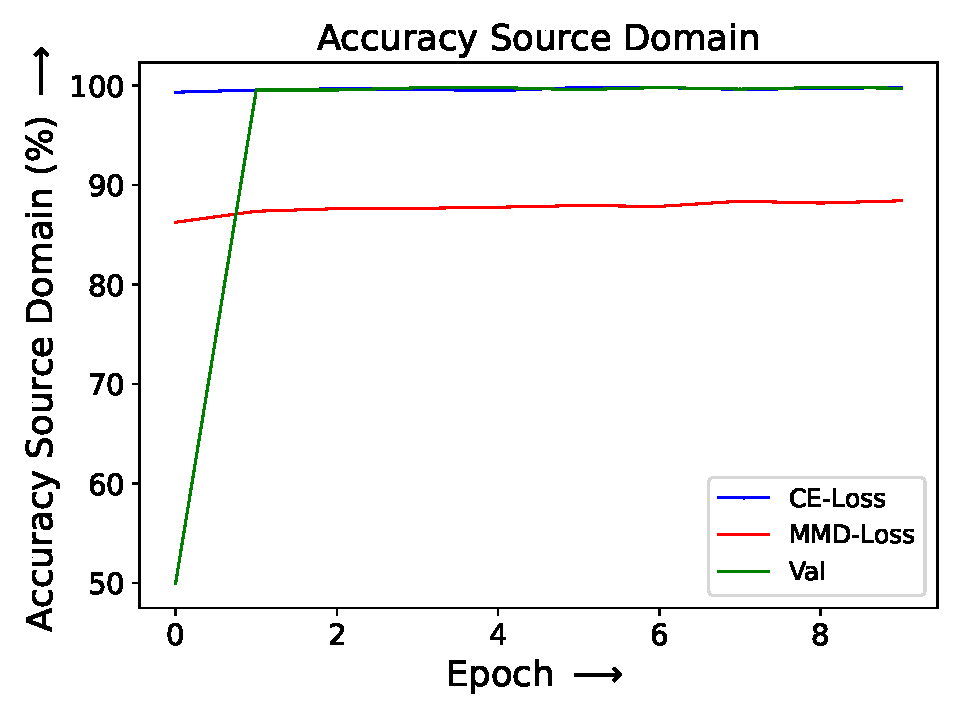
\includegraphics[width=.47\textwidth]{plots_CNN_MMD/Accuracy_Source_Domain_CNN_MMD.pdf}
  \hspace{.3cm}
  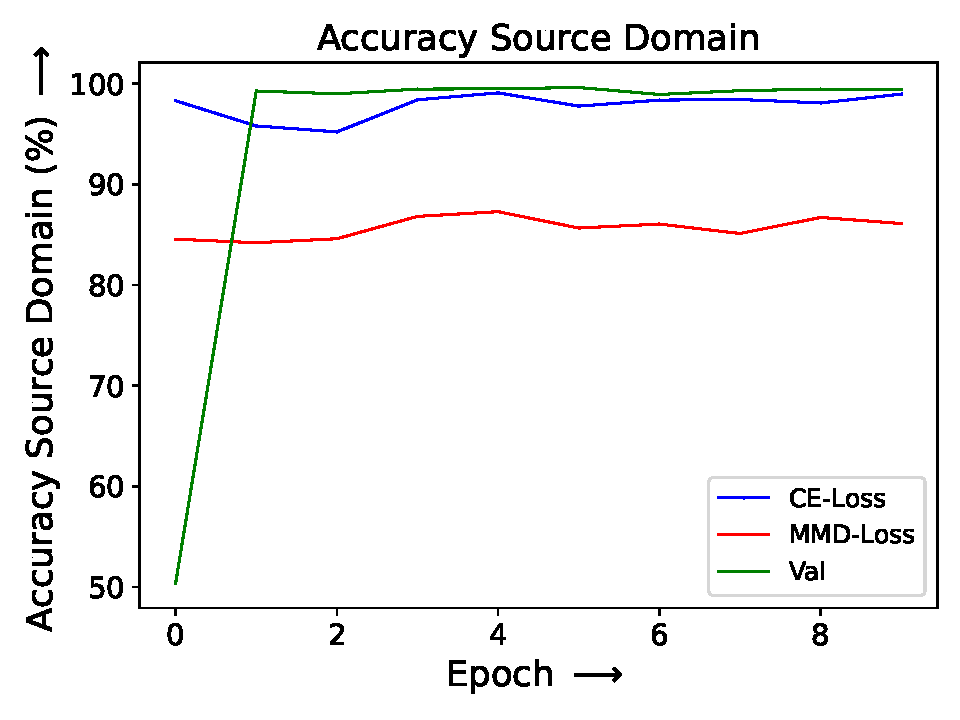
\includegraphics[width=.47\textwidth]{plots_CNN_MMD/Accuracy_Source_Domain_FC_MMD.pdf}

  \vspace{.1cm}

  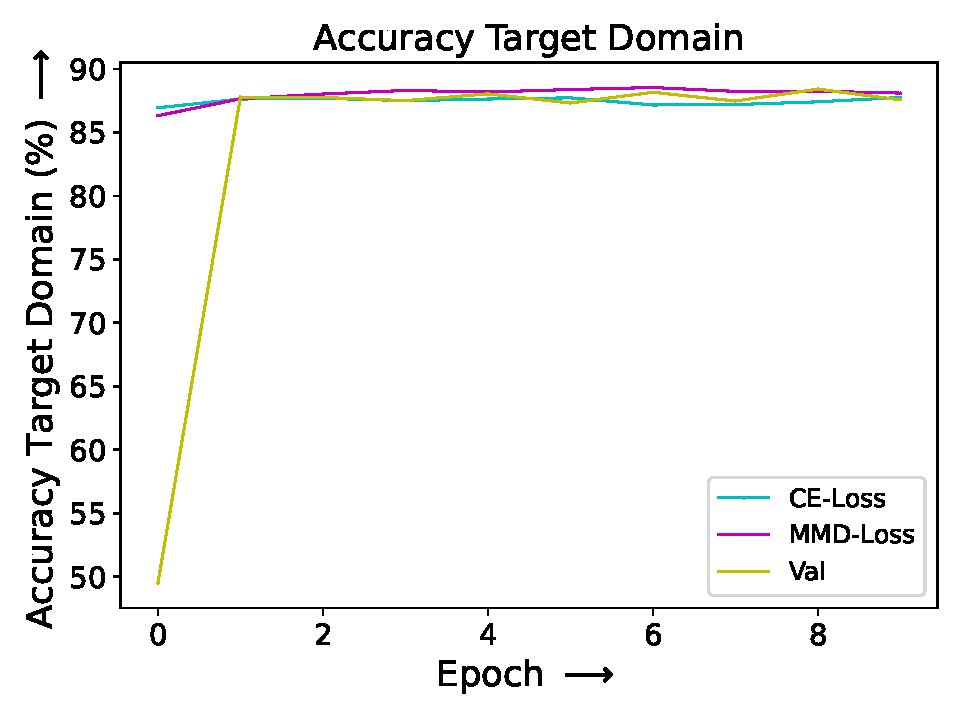
\includegraphics[width=.47\textwidth]{plots_CNN_MMD/Accuracy_Target_Domain_CNN_MMD.pdf}
  \hspace{.3cm}
  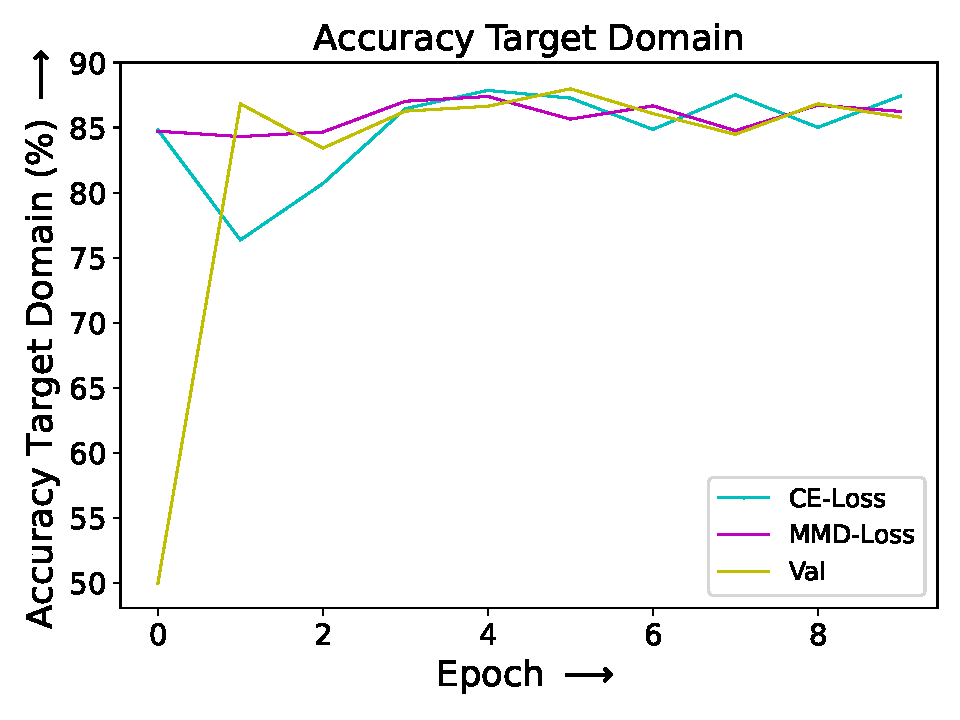
\includegraphics[width=.47\textwidth]{plots_CNN_MMD/Accuracy_Target_Domain_FC_MMD.pdf}

  \caption{Source and Target Accuracy: MMD in CNN (left), MMD in FC (right)}
  \label{fig:accuracy_cnn_and_no_cnn_mmd}
\end{figure}

\begin{figure}[H]
  \centering
  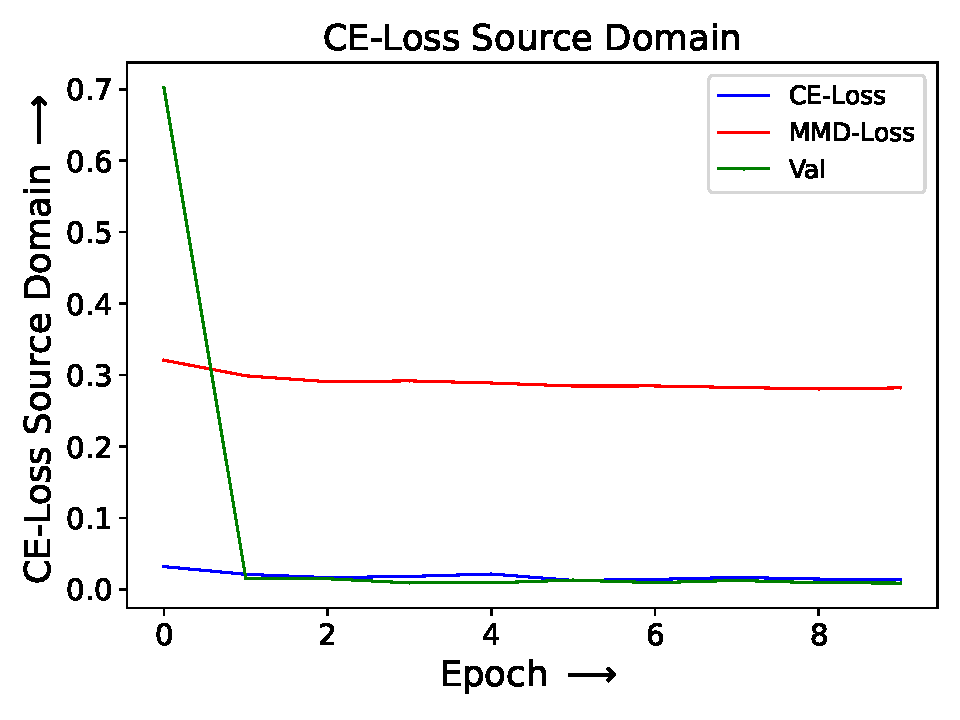
\includegraphics[width=.47\textwidth]{plots_CNN_MMD/CE_Loss_Source_Domain_CNN_MMD.pdf}
  \hspace{.3cm}
  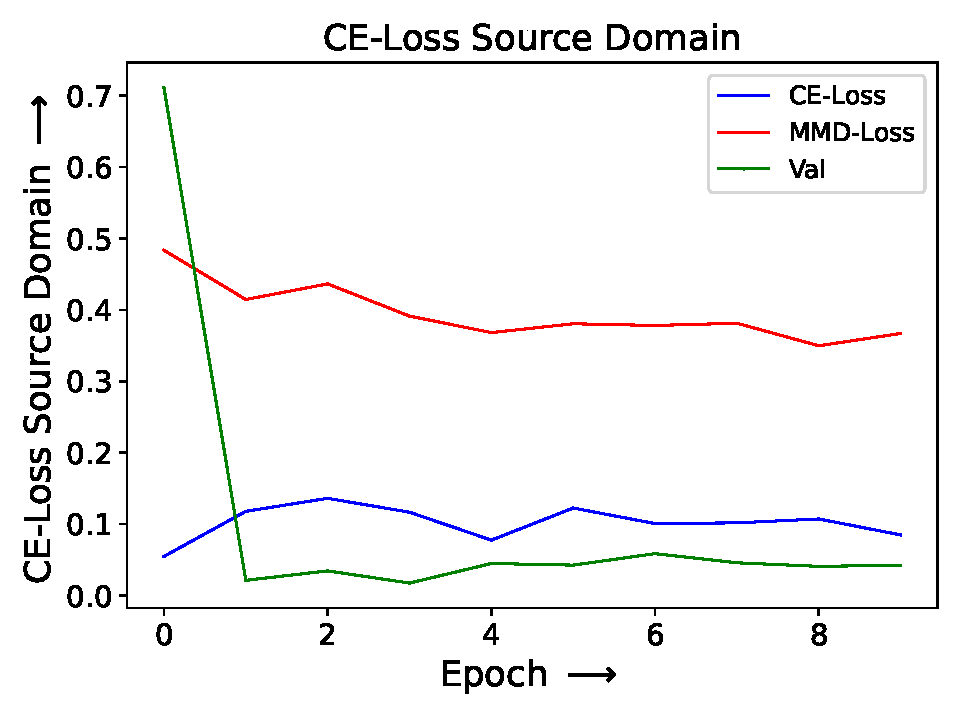
\includegraphics[width=.47\textwidth]{plots_CNN_MMD/CE_Loss_Source_Domain_FC_MMD.pdf}

  \vspace{.1cm}

  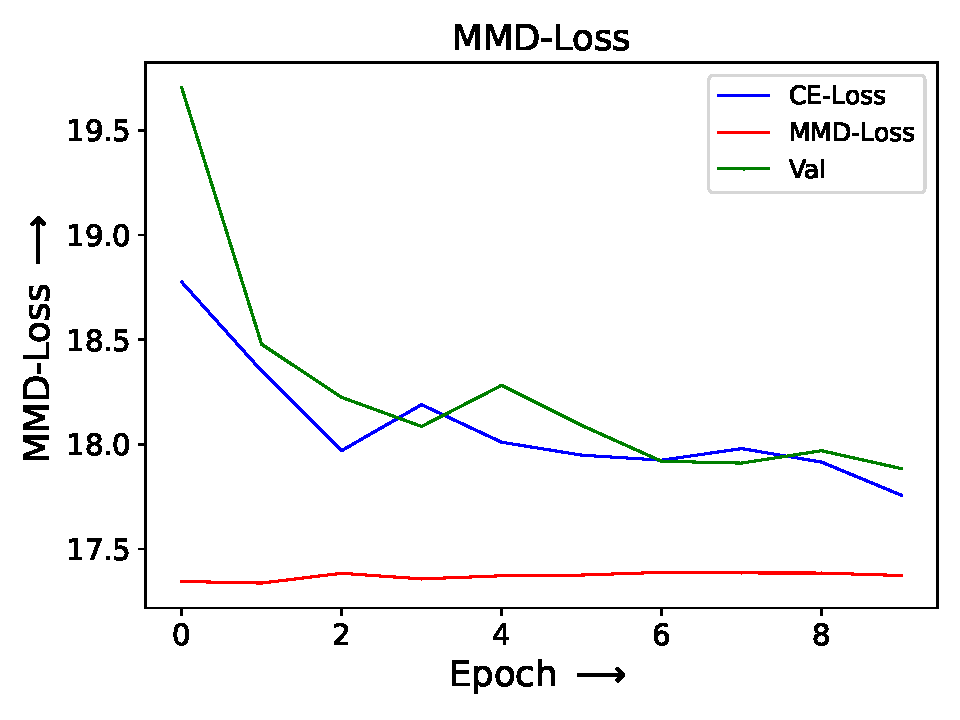
\includegraphics[width=.47\textwidth]{plots_CNN_MMD/MMD_Loss_CNN_MMD.pdf}
  \hspace{.1cm}
  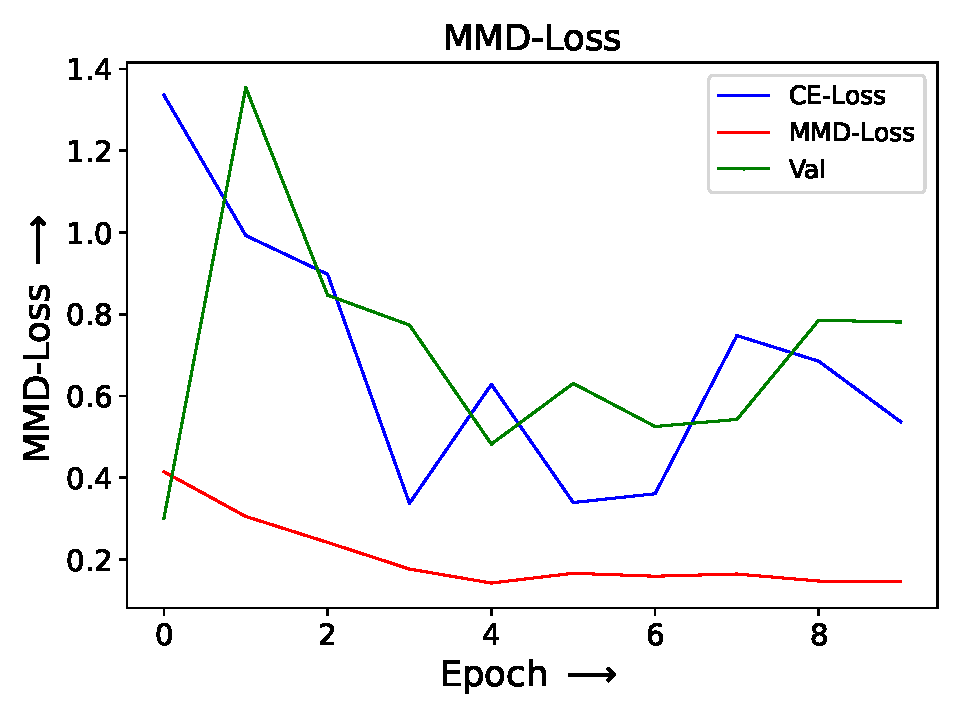
\includegraphics[width=.48\textwidth]{plots_CNN_MMD/MMD_Loss_FC_MMD.pdf}

  \caption{MMD- and CE-Loss: MMD in CNN (left), MMD in FC (right)}
  \label{fig:loss_cnn_and_no_cnn_mmd}
\end{figure}

\section{Real-World Dataset}
In the following section the performance of models trained with different MMD-losses are evaluated on the real-world BSD dataset. The goal of this chapter is to evaluate the benefits and problems of MMD-based domain adaption for PHM of industrial machines. All presented models have the same architecture and optimization strategy but differ in the applied MMD-losses. MMD-losses with different GAMMAs and latent feature space choices were evaluated. In the context of PHM of BSDs, the performance of the MMD-based models are compared with a baseline model, which does not apply any MMD-loss during the training. Table \ref{tab:MMD_layer_choice}  specifies the latent feature space choices included in the different applied MMD-loss types:

\begin {table}[H]
\centering

\begin{tabular}{llllllll}
  \toprule
  Model          & Conv1 & Conv2 & Conv3 & Flatten & FC1 & FC2 \\
  \midrule
  
\vspace{.5cm}

 \parbox[t]{0mm}{\multirow{1}{*}{\rotatebox[origin=c]{90}{\thead{BASE- \\ LINE}}}} & - & - & - & - & - & -\\
 
\vspace{.5cm}

 \parbox[t]{0mm}{\multirow{1}{*}{\rotatebox[origin=c]{90}{\thead{FULL \\ MMD}}}} & \checkmark & \checkmark & - & \checkmark & \checkmark & \checkmark\\
 
\vspace{.5cm}

 \parbox[t]{0mm}{\multirow{1}{*}{\rotatebox[origin=c]{90}{\thead{FC \\ MMD}}}} & - & - & - & \checkmark & \checkmark & \checkmark\\
 
\vspace{.5cm}

 \parbox[t]{0mm}{\multirow{1}{*}{\rotatebox[origin=c]{90}{\thead{CNN \\ MMD}}}} & \checkmark & \checkmark & \checkmark & - & - & -\\

 
  \bottomrule
\end{tabular}

\caption {MMD layer choice of presented models} \label{tab:MMD_layer_choice} 
\end {table}

Similarly to the dummy dataset, the influence of the GAMMA and latent feature space choice on the PHM performance of the developed MMD-based models are examined in the chapters \ref{ch:Influence_GAMMA_real_dataset} and \ref{ch:Influence_Layer_real_dataset}. For several reasons, the previously presented labeled MMD-loss was excluded from this evaluation on the real-world BSD dataset. Firstly, the labeled MMD-loss uses target labels, which in this evaluation no other MMD-loss type does. To achieve good comparability just models with equal conditions and data access during the training are considered in this evaluation. Secondly, optimization methods using target labels are impractical for the real-world use. In domain adaptation tasks, neural networks are first trained on the source domain and afterwards transferred to the target domain. If optimization methods require target labels, one could train the neural networks directly on the target domain. The necessity of target labels prevents the easy model adaptation by solely including the unlabeled target dataset. Labeling a dataset is often done manually and can be quite time consuming. Thirdly, the labeled MMD-loss expects additional hyperparameters. Finding those hyperparameters to tune the labeled MMD-loss is more complicated and expects further experiments. The limited time in this thesis is also a reason why the experiments on the real-world dataset are restricted the unlabeled MMD-loss. In chapter \ref{ch:PHM_performance} the models are compared based on their performance on the real-world BSD dataset. In chapter \ref{ch:Performance_overview} the results from the dummy and real-world BSD dataset are concluded once again. For the implementation of the presented models, PyTorch was used. All computations were performed on a Leibniz Supercomputing Centre7 compute node virtual machine with 20
Intel® Xeon® Gold 6148 vCPUs, one Nvidia® Tesla V100, 368 GB RAM, PyTorch v.1.4.0 and CUDA 10.1.


\subsection{Influence of GAMMA Choice on the PHM Performance}\label{ch:Influence_GAMMA_real_dataset}

In the following 3 models were trained with the FULL MMD-loss and different GAMMAs (0, 0.05, 1) on the  D:P mech./X signal for 100 epochs. Similarly to the dummy dataset, the MMD-based model training is very sensitive to the GAMMA choice. Just when the GAMMA is chosen carefully, the domain discrepancy in the hidden layers can be reduced without decreasing the separability between the classes of source and target domain. Fig. \ref{fig:distribution_GAMMA_influence_real_data} shows the latent feature representation of the source and target domain samples in the FC2 layer. A GAMMA of 0.05 is a suitable choice for reducing the domain discrepancy while guaranteeing a sufficient compactness and separability of the source and target classes. From the plots it is hard to make comparisons about the separability and compactness between different GAMMA choices. For a GAMMA of 0.05, the structure of the data distribution seems to be clearer and smoother. This rises the assumption, that separating the classes in this scenario is easier. Especially the class 1 seems to be more compact in both domains when picking a GAMMA of 0.05. When choosing a GAMMA of 1 the MMD-loss becomes too dominant. Noise and unimportant information are transferred between the domains. The MMD-loss reduces the distance between source and target samples from all classes. This destroys the class structure of the source and target domain, which makes the classification task impossible. In this case the feature representations of all samples collapse to a small latent feature subspace.

\begin{figure}[H]
  \centering
  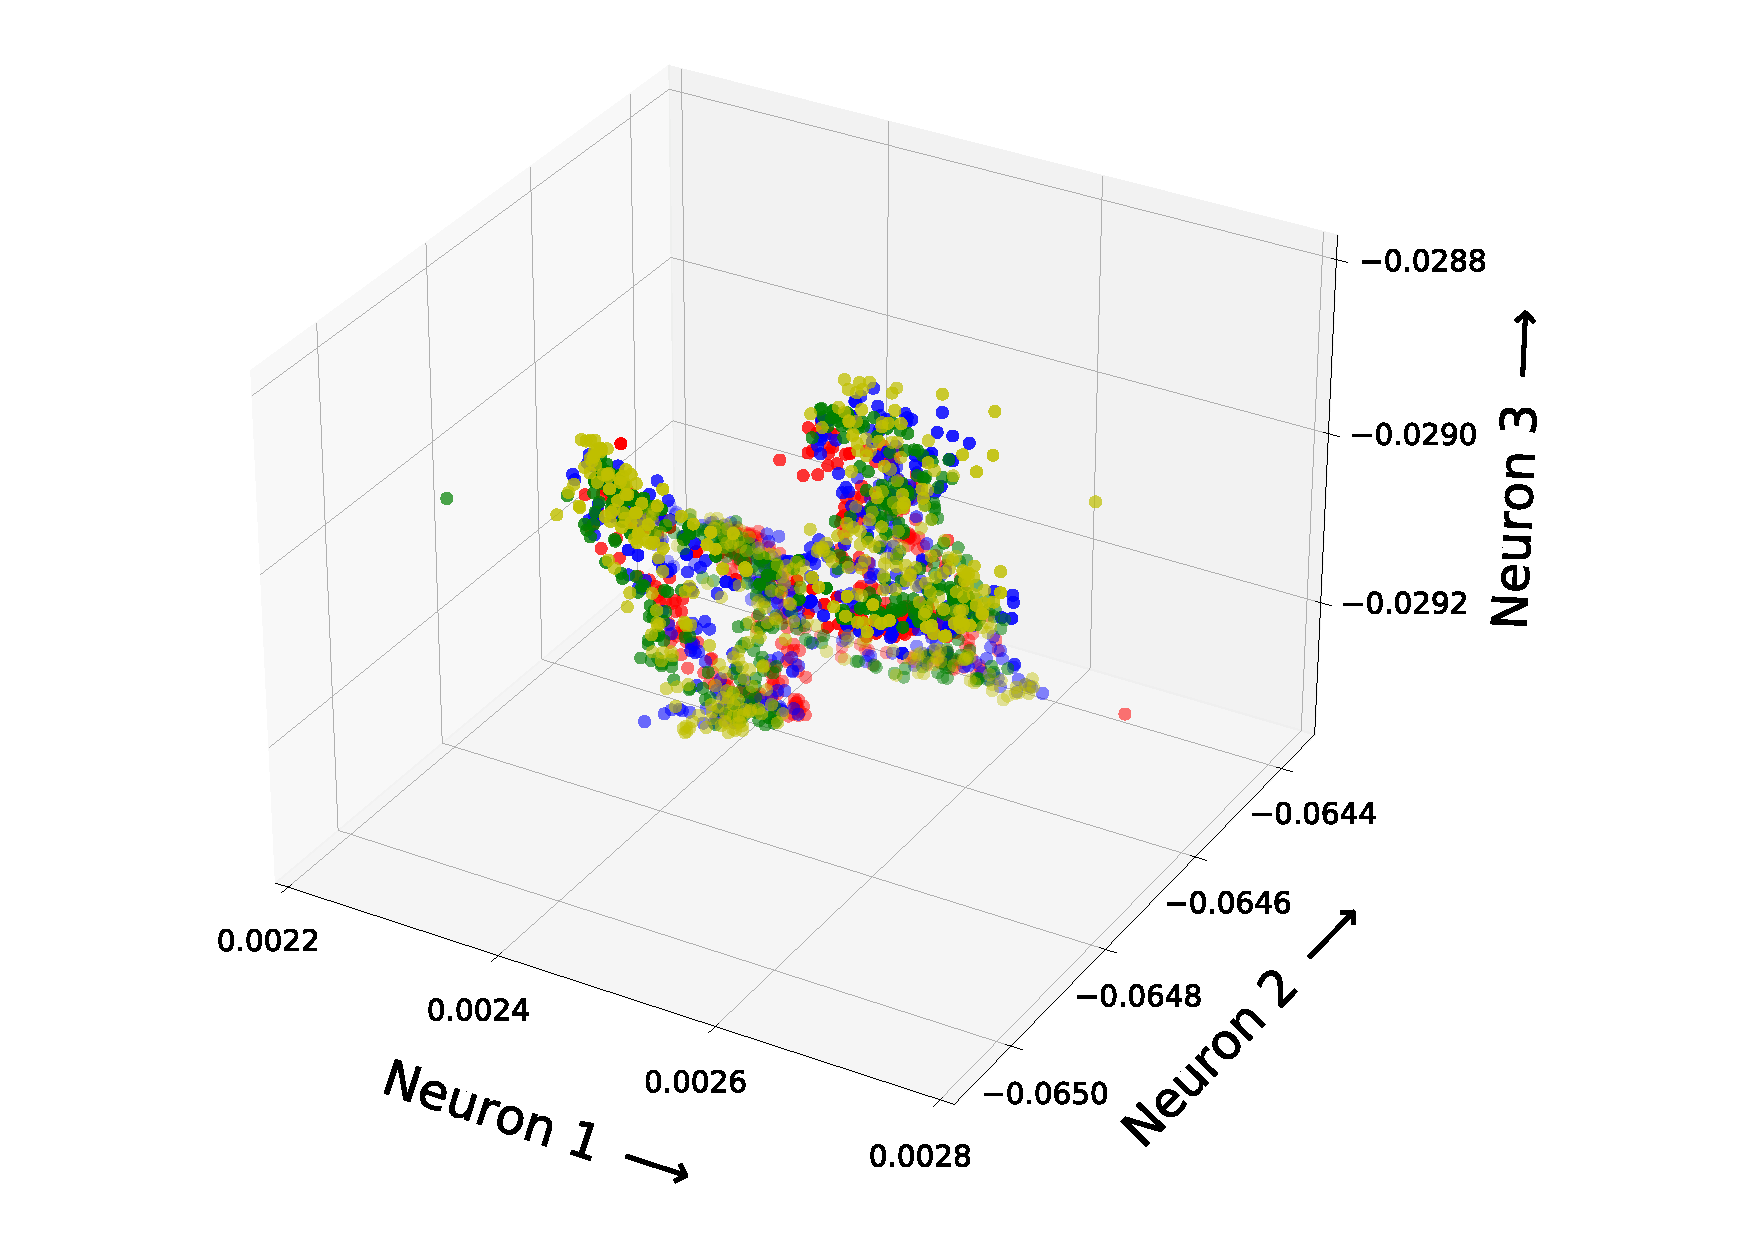
\includegraphics[width=.47\textwidth]{GAMMA_Influence_real_data/P_mech_X_data_distribution_0_GAMMA_0_0.pdf}
  \hspace{.4cm}
  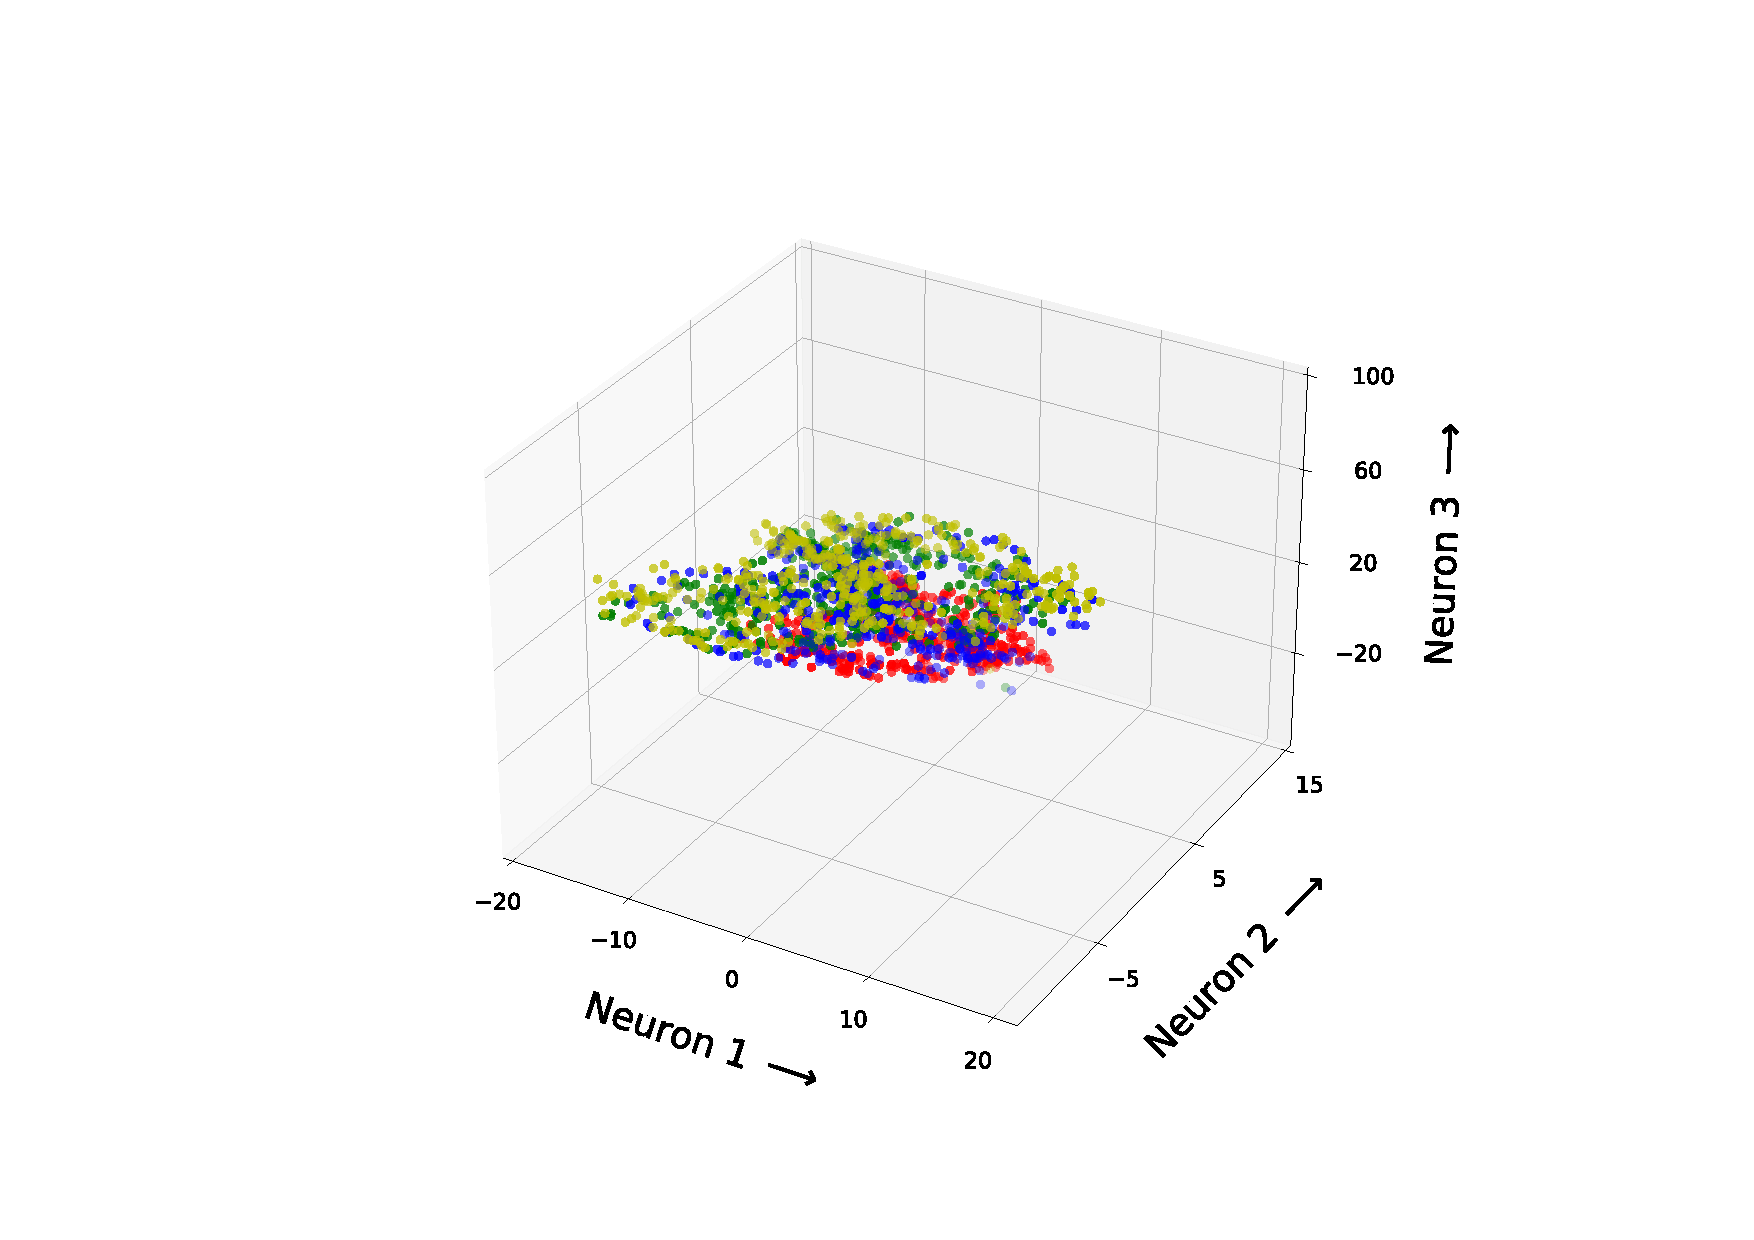
\includegraphics[width=.47\textwidth]{GAMMA_Influence_real_data/P_mech_X_data_distribution_80_GAMMA_0_0.pdf}

  \vspace{.1cm}

  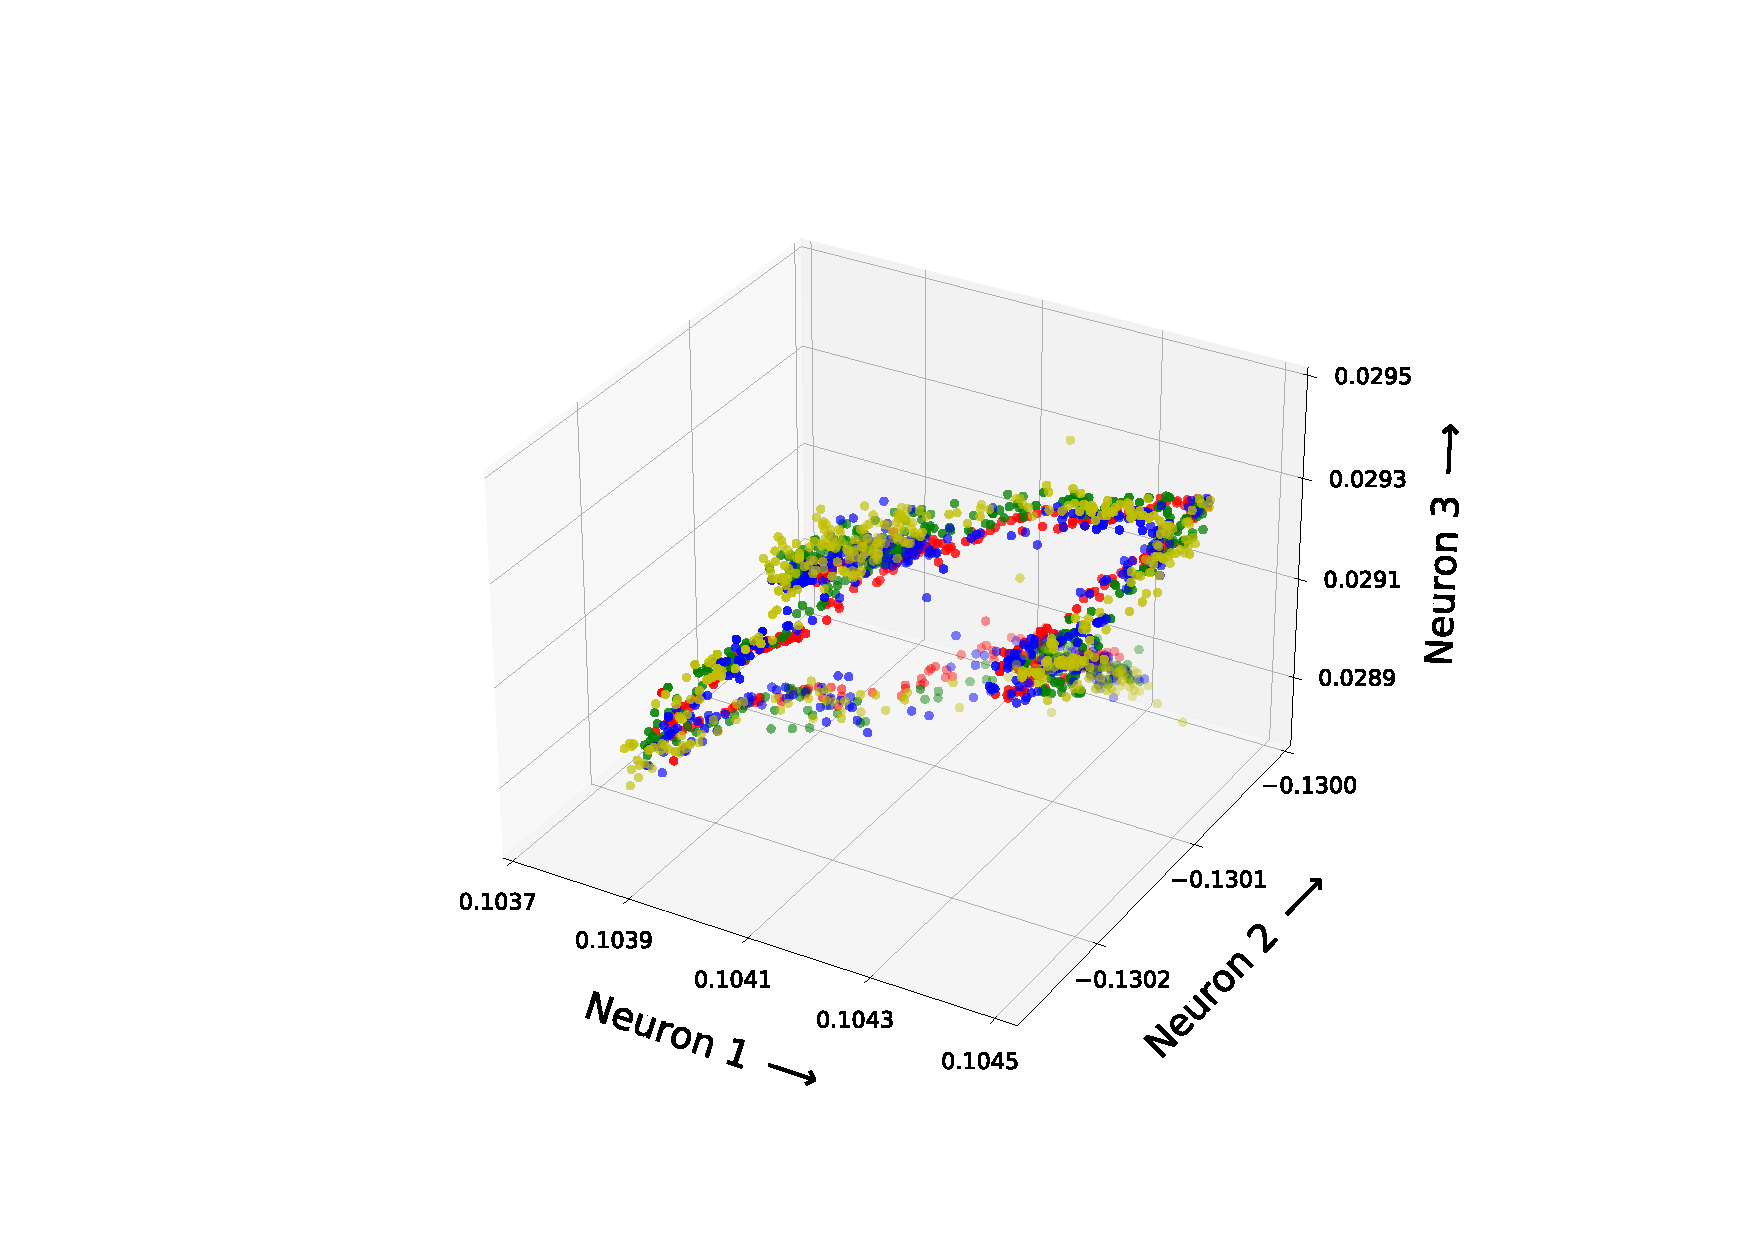
\includegraphics[width=.47\textwidth]{GAMMA_Influence_real_data/P_mech_X_data_distribution_0_GAMMA_0_05.pdf}
  \hspace{.4cm}
  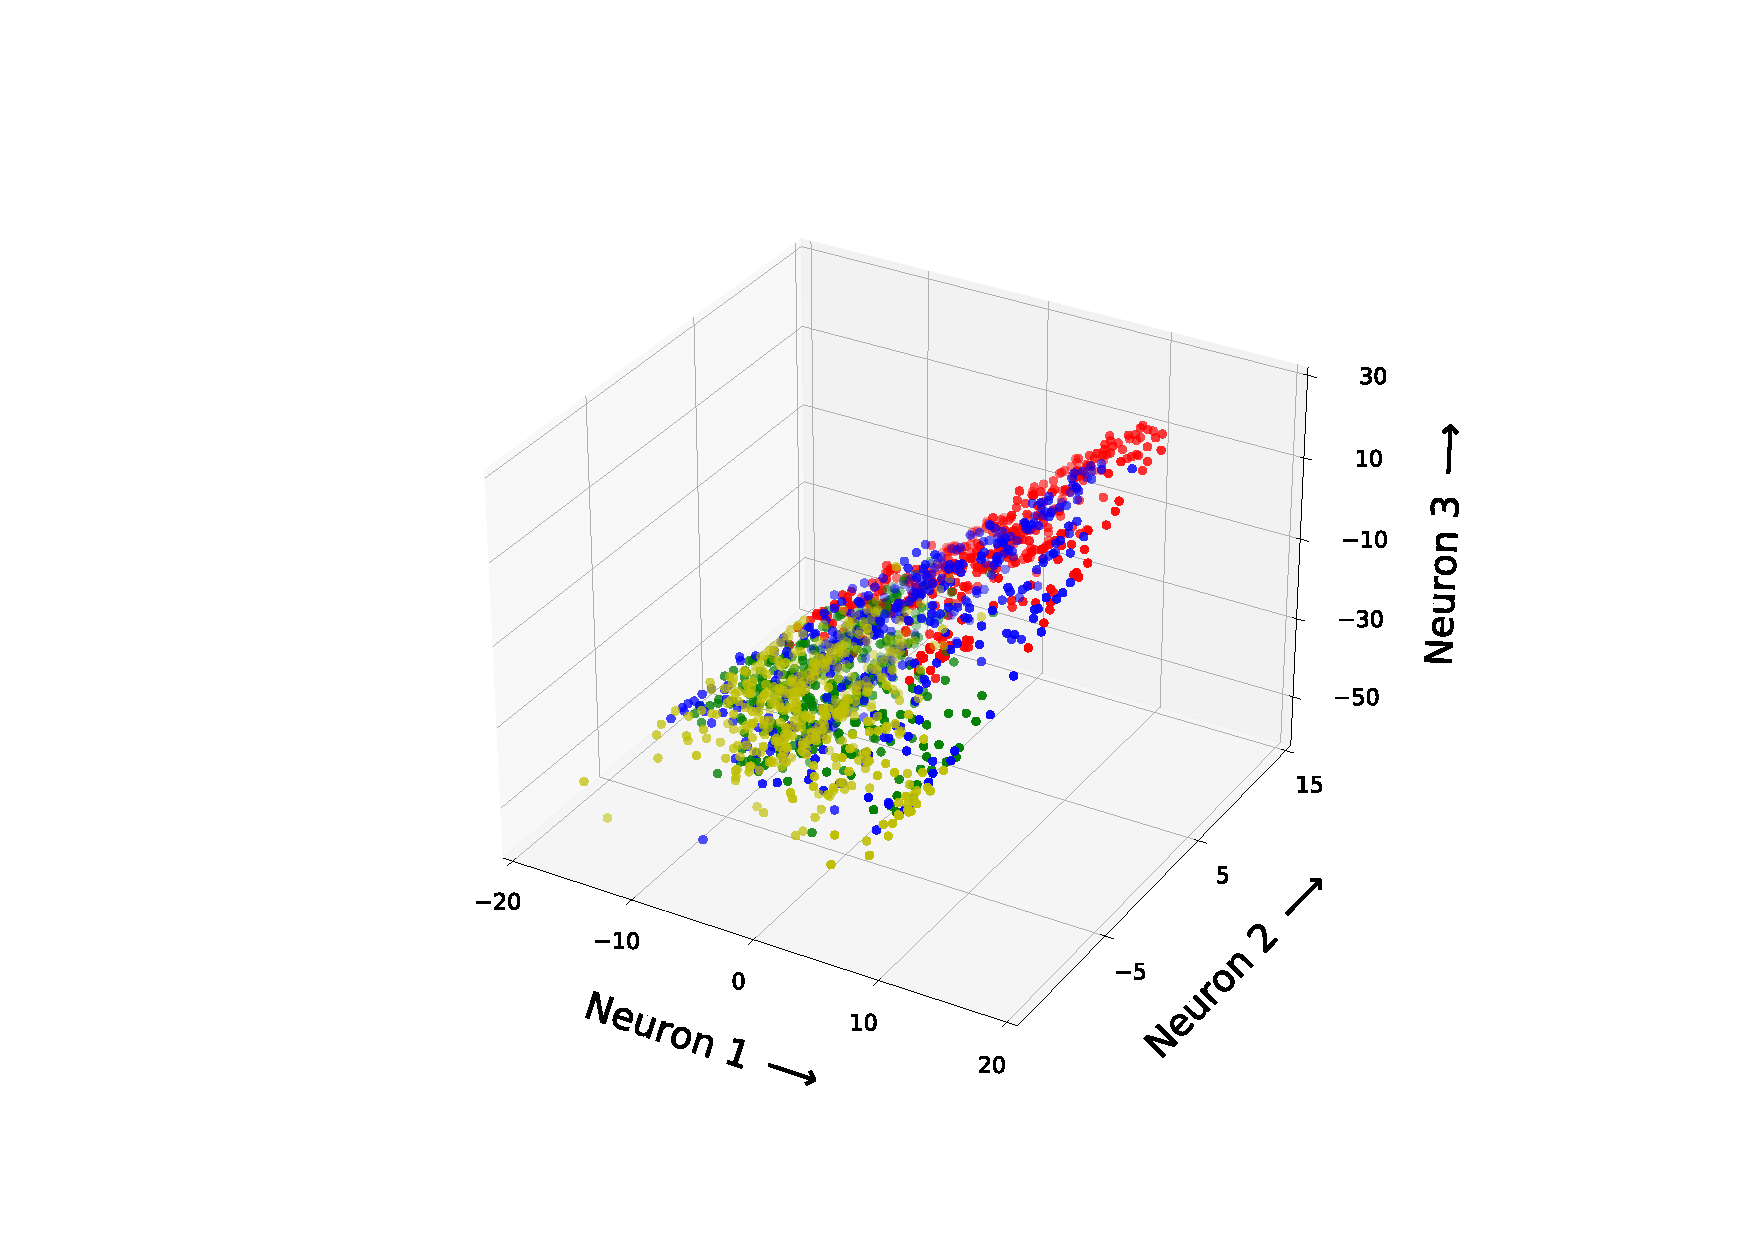
\includegraphics[width=.47\textwidth]{GAMMA_Influence_real_data/P_mech_X_data_distribution_80_GAMMA_0_05.pdf}

  \vspace{.1cm}

  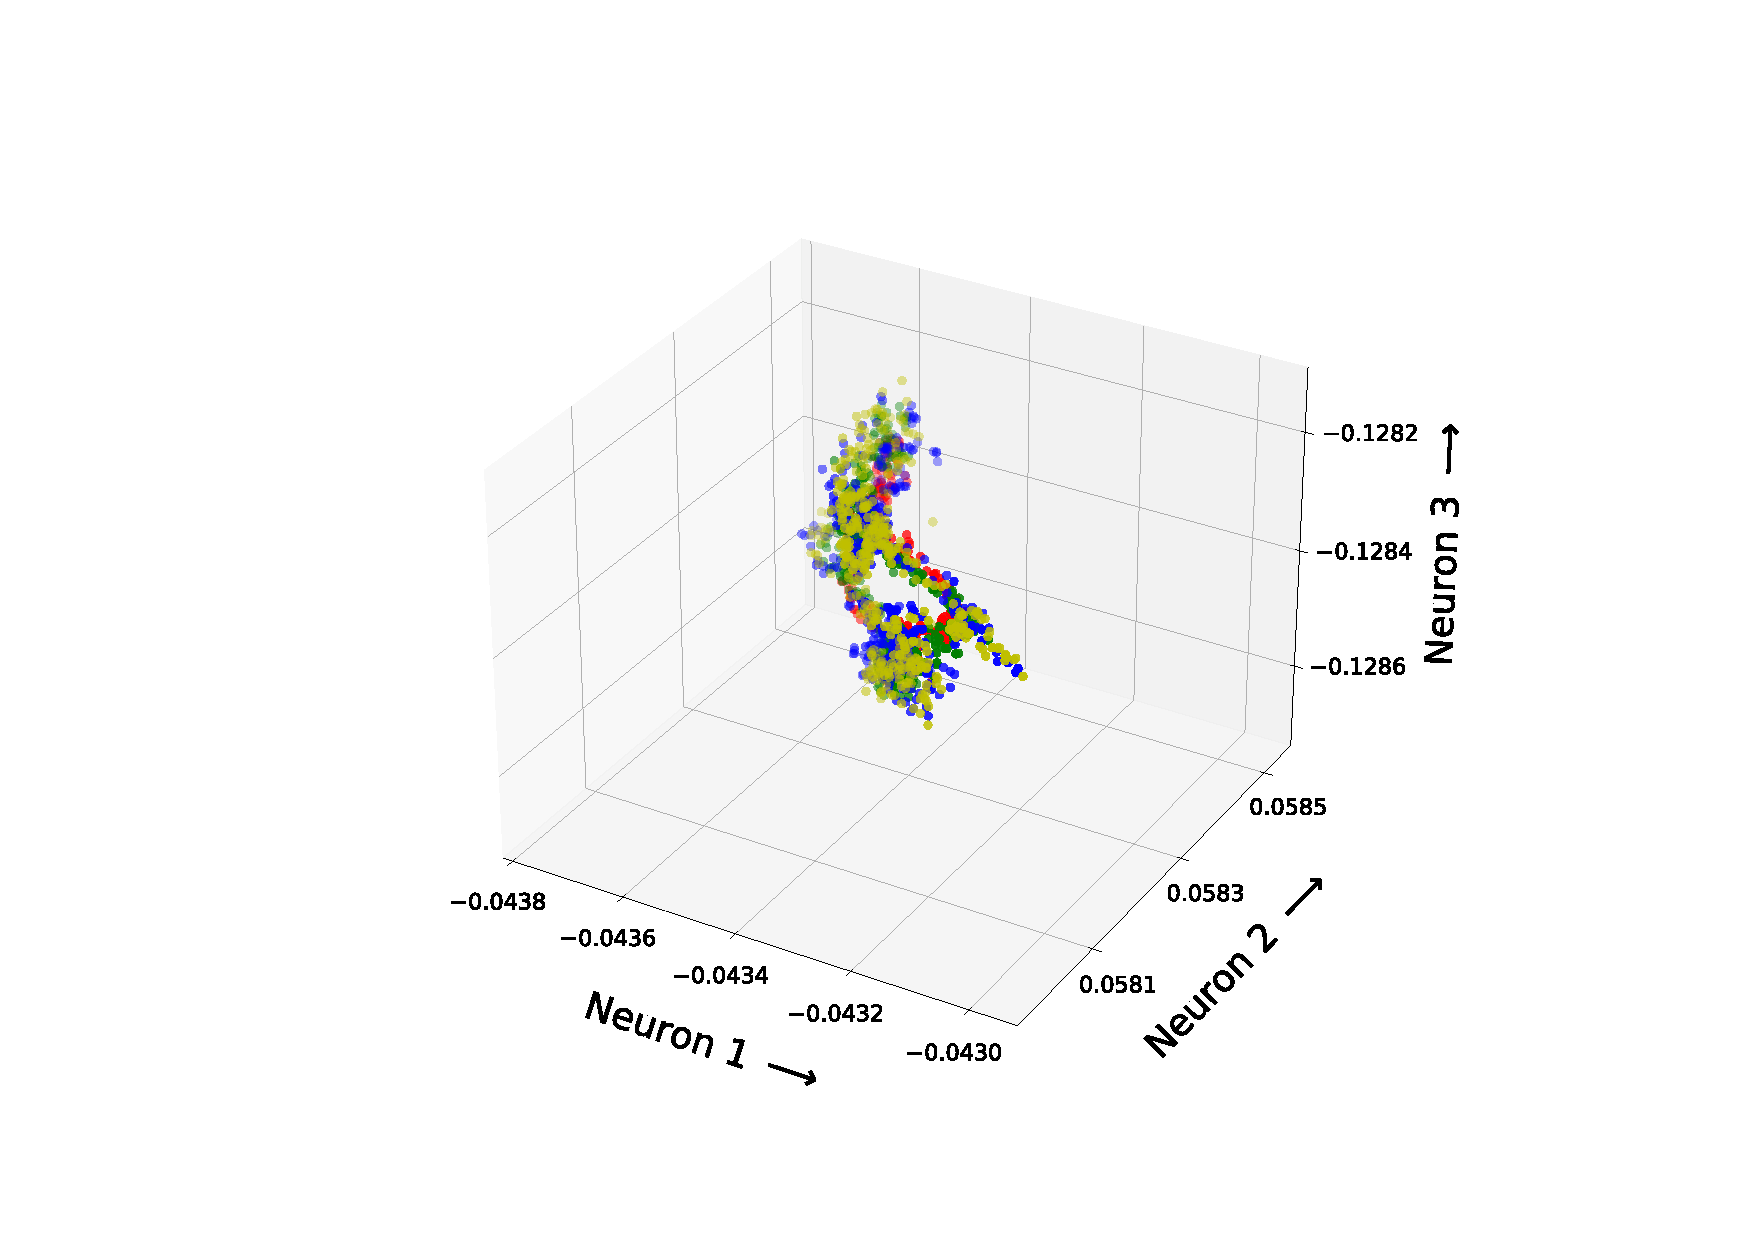
\includegraphics[width=.47\textwidth]{GAMMA_Influence_real_data/P_mech_X_data_distribution_0_GAMMA_1_0.pdf}
  \hspace{.4cm}
  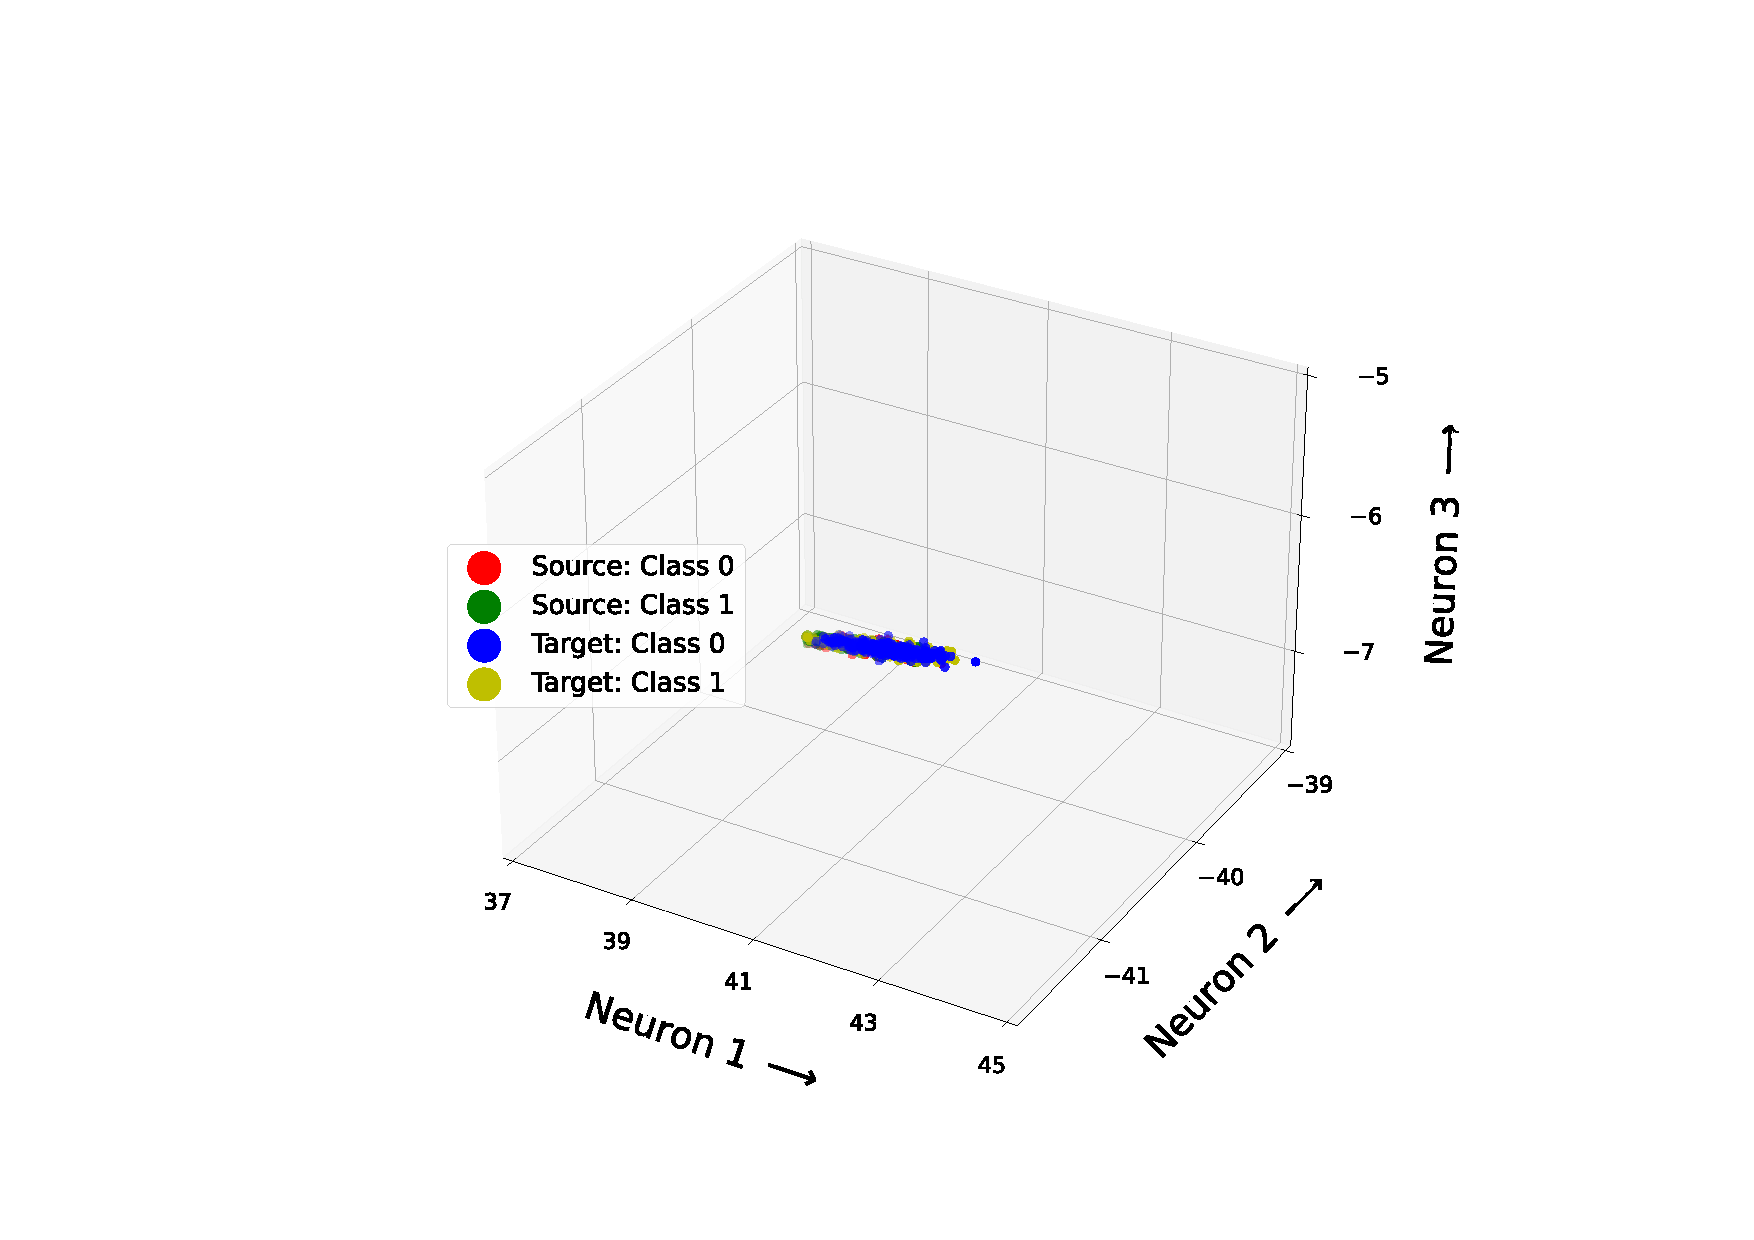
\includegraphics[width=.47\textwidth]{GAMMA_Influence_real_data/P_mech_X_data_distribution_80_GAMMA_1_0.pdf}

  \vspace{.1cm}

  \caption{Data  distribution:  Influence  of  GAMMA  on  Training with D:P\_mech./X:  GAMMA  =  0  (top), GAMMA = 0.05 (middle), GAMMA = 1 (bottom), Epoch 0 (left), Epoch 100 (right)}
  \label{fig:distribution_GAMMA_influence_real_data}
\end{figure}


\subsection{Influence of Latent Feature Space Choice on the PHM Performance}\label{ch:Influence_Layer_real_dataset}
This section analyses the effects of different latent feature space choices on the MMD-based model training. All models were trained with a GAMMA of 1 on the D:I soll/X signal for 100 epochs. Each model training was repeated 5 times. Fig. \ref{fig:target_accuracy_MMD_layer} shows the corresponding development of the target accuracies. When the MMD-loss is just applied in the FC layers, the training collapses in 2 of the 5 experiments (row 3 $\&$ 5). In the other 3 cases the accuracy has the slight tendency to decrease during the training. The CNN MMD-based model training shows worse reproducibility throughout the 5 experiments than the FULL MMD-based model training. Often, the fluctuations on the validation data are not reduced properly throughout the training (row 1 $\&$ 4 $\&$ 5). Especially towards the end of the training, the FULL MMD-based model training seems to be more stable. Anyhow, minor fluctuations are also observable for the FULL MMD-based model training (row 3 $\&$ 4). In this thesis the final model is picked based on its performance on the validation dataset of the target domain. In real world scenarios, the target labels are often unknown. Oftentimes, the model in the end of the training is picked as the final one. When the model performance decreases or fluctuates throughout the training, the best possible model will not be found. For this reason a stable model training should not be underestimated. A more detailed description of how the final models are picked is given in chapter \ref{ch:PHM_performance}. 

\begin{figure}[H]
  \centering

  \includegraphics[width=.32\textwidth]{MMD_LAYER_influence_real_data/CNN_MMD/Accuracy_Target_Domain_1.pdf}
  \hspace{.1cm}
  \includegraphics[width=.32\textwidth]{MMD_LAYER_influence_real_data/FC_MMD/Accuracy_Target_Domain_1.pdf}
  \hspace{.1cm}
  \includegraphics[width=.32\textwidth]{MMD_LAYER_influence_real_data/FULL_MMD/Accuracy_Target_Domain_1.pdf}

  \vspace{.3cm}

  \includegraphics[width=.32\textwidth]{MMD_LAYER_influence_real_data/CNN_MMD/Accuracy_Target_Domain_2.pdf}
  \hspace{.1cm}
  \includegraphics[width=.32\textwidth]{MMD_LAYER_influence_real_data/FC_MMD/Accuracy_Target_Domain_2.pdf}
  \hspace{.1cm}
  \includegraphics[width=.32\textwidth]{MMD_LAYER_influence_real_data/FULL_MMD/Accuracy_Target_Domain_2.pdf}

  \vspace{.3cm}

  \includegraphics[width=.32\textwidth]{MMD_LAYER_influence_real_data/CNN_MMD/Accuracy_Target_Domain_3.pdf}
  \hspace{.1cm}
  \includegraphics[width=.32\textwidth]{MMD_LAYER_influence_real_data/FC_MMD/Accuracy_Target_Domain_3.pdf}
  \hspace{.1cm}
  \includegraphics[width=.32\textwidth]{MMD_LAYER_influence_real_data/FULL_MMD/Accuracy_Target_Domain_3.pdf}
  
    \vspace{.3cm}

  \includegraphics[width=.32\textwidth]{MMD_LAYER_influence_real_data/CNN_MMD/Accuracy_Target_Domain_4.pdf}
  \hspace{.1cm}
  \includegraphics[width=.32\textwidth]{MMD_LAYER_influence_real_data/FC_MMD/Accuracy_Target_Domain_4.pdf}
  \hspace{.1cm}
  \includegraphics[width=.32\textwidth]{MMD_LAYER_influence_real_data/FULL_MMD/Accuracy_Target_Domain_4.pdf}
  
    \vspace{.3cm}
    
  \includegraphics[width=.32\textwidth]{MMD_LAYER_influence_real_data/CNN_MMD/Accuracy_Target_Domain_5.pdf}
  \hspace{.1cm}
  \includegraphics[width=.32\textwidth]{MMD_LAYER_influence_real_data/FC_MMD/Accuracy_Target_Domain_5.pdf}
  \hspace{.1cm}
  \includegraphics[width=.32\textwidth]{MMD_LAYER_influence_real_data/FULL_MMD/Accuracy_Target_Domain_5.pdf}


  \caption{Target Accuracy: Influence of MMD layer Choice on Training: CNN MMD (left), FC MMD (middle), FULL MMD (right)}
  \label{fig:target_accuracy_MMD_layer}
\end{figure}


\section{Overal PHM Performance}\label{ch:PHM_performance}
By evaluating models trained with different MMD-loss types, the utility and applicability of MMD-based model training for real-world PHM tasks is evaluated in this chapter. In a first step, all of the 49 signals are evaluated for their suitability in PHM systems. For this, models are trained on these signals without applying any MMD-loss. Based on the performance of these models, 7 promising signals are picked for further testing. In a second step, a MMD-based model training is applied on these 7 signals. Models are optimized with FULL MMD-, FC MMD- and CNN MMD-losses and 3 different GAMMAs (0.05 $\&$ 0.5 $\&$ 1). All 9 MMD-based model training (all combinations of MMD types and GAMMAs) and the baseline model training, which does not apply any MMD-loss, are repeated 5 times on each of the 7 signals. In each epoch during the MMD-based model training, the models are evaluated based on the balanced accuracy on the target domain validation dataset. Throughout the training the best performing model is stored. The different MMD-loss types are compared based on the performance of those stored models on the unseen target domain test dataset. From 5 equally executed model training the average accuracy of the corresponding  models on the target domain test dataset is shown in table \ref{tab:Mean_Accuracy}. For 4 of the 7 signals the FULL MMD and for the other 3 the CNN MMD models perform best. The FC MMD models never outperforms the other MMD-based models. Compared to the baseline model the MMD-based models are able to increase the accuracy by up to 10.18$\%$. Table \ref{tab:Variance_Accuracy} shows the target accuracy variances for all models on the selected signals. The best performing model usually shows low to average variances. A low variance verifies a high degree of reproducibility throughout the repeated experiments. This demonstrates the meaningfulness of the results and proves the applicability and utility of MMD-losses for reducing the domain discrepancy in PHM related tasks. Table \ref{tab:Average_Variance_Accuracy} shows the average variance over each of the 105 MMD-based models (7 signals, 3 GAMMAs, 5 experiments) and over the 35 baseline models (7 signals, 5 experiments). From the MMD-based models, the FULL MMD models has the lowest and the FC MMD models the highest average target accuracy variance. This shows, that the FULL MMD models have the highest consistency throughout the executed experiments performed with varying GAMMAs on different signals. The FULL MMD models seem to be more robust and less sensible to GAMMA and signal choices. As mentioned in the results of the dummy dataset, a reason for the inconsistency of the FC MMD models might be the contradicting training goals when evaluating the MMD- as well as the source CE-loss just in the FC layers. The shifting focus on different training goals during the training might lead to instabilities. In such cases, the training is more prone to get stuck in local minima.
\begin{comment}
Windowing functions split the recorded data in shorter sequences. The generated windows should capture the degradation related patterns of the vibration signals. For this reason, the windows should be adapted according to the consistency and periodicity of the data. In this thesis a window size of 1024 was chosen. The windowing requirements are different for the different machine excitements (constant speed excitement, direction change excitement and sweep excitement). The windows are too short to capture one whole period of of forward and backward motion in the data recorded during constant speed machine excitement. The data can be separated in phases of constant speed and direction change, which each contains roughly 1000 datapoints. The windows are of equal size as the described phases in the data. Since the windows are not synchronized with those phases, they overlap to a large extent but do not cover them perfectly. The windows are big enough to capture several periods of forward and backward movements in data recorded during direction change excitement. When exciting the machine with a sweep signal the PHM system should better process the whole corresponding vibration signal. It is important to capture the changing frequencies and amplitudes during the complete sweep excitement. The best PHM results were achieved on data recorded during constant speed and  direction change excitement of the machine. This shows that the windowing did not work very well on the data recorded during sweep excitement. Generally, when choosing the window size, there is a trade-off between the window size and the number of windows generated from the data. Both extremes (few big windows and numerous small windows) might lead to problems during the training. The PHM results can probably be improved by an intelligent and adaptive preprocessing to generate suitable and synchronized data windows. Azamfat et al \cite{AZAMFAR2020103932} present such an approach. They apply a constant excitement to the machine and separate the data BSD phases of constant velocity direction change movement. The PHM system just relies on the data recorded during BSD constant velocity. The signals D:I\_ist/X (actual electrical power), D:I\_soll/X (target electrical power) and D:P\_mech./X (mechanical power) coming from the controller show high potential for the PHM task. The most suitable accelerometer installation is the one on the BSD nut. Pandahare et al \cite{Pandhare2021} discovered similar results. Often in real operational scenarios such an installation is impractical \cite{Pandhare2021}. Alternatively to the BSD nut position, this thesis shows, that the top LGS achieves better PHM results than the bottom one.
\end{comment}


\begin{sidewaystable}
\begin {table}[H]
\centering
\begin{tabular}{llllllllll}
  \toprule
  Model          & GAMMA    & D:I\_ist/X & D:I\_soll/X & D:P\_mech./X & C:z\_top & C:z\_nut & D:x\_nut & D:z\_top \\
  \midrule
  
  \vspace{1cm}
  
    \thead{BASE- \\ LINE}  & -      & 70.08 & 75.62 & 74.7 & 69.14 & 57.4 & 58.74 & 57.88\\


 
                            & 0.05   & 71.56 & 75.42 & \textbf{78.96} & 72.36 & 58.10 & 49.52 & \textbf{62,64}\\
    \thead{FULL \\ MMD}     & 0.5    & 73.78 & 74.84 & 52.78 & \textbf{75.92} & \textbf{64.76} & 50.52 & 49,94\\
    
    \vspace{1cm}
    
                            & 1      & 72.98 & 75.18 & 49.80 & 74.12 & 57.02 & 50.62 & 50.52\\


                            & 0.05   & 73.60 & 76.38 & 74.98 & 71.36 & 57.48 & 52.44 & 61.3\\
    \thead{FC \\ MMD}       & 0.5    & 70.74 & 74.86 & 72.62 & 69.32 & 59.76 & 50.12 & 53.22\\
    
    \vspace{1cm}
    
                            & 1      & 73.42 & 65.46 & 76.96 & 62.34 & 58.86 & 50.92 & 53.96\\

                            & 0.05   & 71.62 & \textbf{76.44} & 51.80 & 73.20 & 59.30 & 58.04 & 53.82\\
    \thead{CNN \\ MMD}      & 0.5    & \textbf{73.90} & 75.86 & 51.58 & 72.28 & 55.76 & 68.04 & 51.72\\
                            & 1      & 73.80 & 73.82 & 51.12 & 72.18 & 54.28 & \textbf{68.92} & 51.28\\
 \addlinespace
 \hline
 \thead{MMD\\GAIN:} &  & +3.82 & +0.82 & +4.26 & +6.78 & +7.36 & +10.18 & +4.76\\
 
  \bottomrule
\end{tabular}
\caption {Mean target test accuracy (\%)} \label{tab:Mean_Accuracy} 
\end {table}
\end{sidewaystable}

\begin{sidewaystable}
\begin {table}[H]
\centering
\begin{tabular}{llllllllll}
  \toprule
  Model          & GAMMA    & D:I\_ist/X & D:I\_soll/X & D:P\_mech./X & C:z\_top & C:z\_nut & D:x\_nut & D:z\_top  \\
  \midrule

    \vspace{1cm}

    \thead{BASE- \\ LINE}   & -      & 2.07 & 0.27 & 2.20 & 2.55 & 1.11 & 1.04 & 1.22\\
 
                            & 0.05   & 1.06 & 0.74 & \textbf{1.79} & 1.80 & 2.04 & 1.39 & \textbf{2.48}\\
    \thead{FULL \\ MMD}     & 0.5    & 0.72 & 1.44 & 3.33 & \textbf{1.72} & \textbf{1.42} & 1.23 & 1.02\\
    
    \vspace{1cm}  
    
                            & 1      & 0.76 & 0.81 & 0.87 & 6.06 & 5.57 & 0.96 & 0.79\\



                            & 0.05   & 1.96 & 0.61 & 1.86 & 1.82 & 1.63 & 3.86 & 1.60\\
    \thead{FC \\ MMD}       & 0.5    & 1.34 & 0.72 & 11.06 & 6.42 & 2.28 & 0.45 & 3.14\\
    
    \vspace{1cm}
    
                            & 1      & 0.96 & 12.01 & 5.46 & 8.18 & 2.13 & 0.93 & 2.70\\
                            & 0.05   & 2.13 & \textbf{0.53} & 2.39 & 1.12 & 4.01 & 4.18 & 7.26\\
    \thead{CNN \\ MMD}      & 0.5    & \textbf{0.25} & 1.57 & 1.08 & 1.22 & 3.27 & 3.51 & 3.22\\
                            & 1      & 0.51 & 1.25 & 2.02 & 2.51 & 4.54 & \textbf{2.54} & 2.34\\
  \bottomrule
\end{tabular}
\caption {Standard deviation target test accuracy (\%)} \label{tab:Variance_Accuracy} 
\end {table}
\end{sidewaystable}


\begin {table}[H]
\centering
\begin{tabular}{lllll}
  \toprule
  Model & BASE-LINE & FULL MMD & FC MMD & CNN MMD\\
  \midrule
  AVG VARIANCE & 1.50 & 1.81 & 3.39 & 2.45\\
  \bottomrule
\end{tabular}
\caption {Average standard deviation target test accuracy (\%)} \label{tab:Average_Variance_Accuracy} 
\end {table}

\section{Conclusion}\label{ch:Performance_overview}
In the following chapter, the findings from the experiments in the dummy and real-world dataset are summarized once again. Variations in the underlying functionality and mechanism of different MMD-loss types became especially visible in the dummy dataset. The overall performance differences of the MMD-loss types were evaluated on the real-world dataset. The labeled MMD-loss highlights the deficits of the unlabeled MMD-loss. The labeled MMD-loss separately optimizes the domain discrepancy of samples from different and same classes. This helps to improve the compactness and separability of all classes while reducing the discrepancy between the domains. The necessity for target labels, makes the labeled MMD-loss impractical for the real-world use. For this reasons the labeled MMD-loss was not further evaluated on the real-world dataset. Since the unlabeled MMD loss has no access to the target labels, class specific properties like the compactness and separability can not be optimized for the target domain. The unlabeled MMD-loss reduces the discrepancy between samples of different domains without considering their class labels. Therefore, the model optimization with the unlabeled MMD-loss is more prone to reduce the separability while reducing the domain discrepancy. This can lead to trivial solutions, where the feature representation of all samples collapse to a small subset. The experiments on the real-world dataset showed, that the MMD-losses applied in early CNN layers reduce the domain discrepancy more efficiently and therefore outperformed those restricted to the FC layers. The model optimization with those MMD-losses showed less fluctuation and higher reproducability throughout several equally repeated experiments. The increased consistency and robustness of those MMD-losses was proved by the low test accuracy variance averaged over experiments performed on different signals and with different GAMMAs. Compared to the baseline model, which does not apply any MMD loss, the PHM accuracy was improved by all MMD-loss types. For all evaluated signals, the GAMMA choice was highly relevant and decided about the performance gain achieved by the MMD-loss. The GAMMA had to be picked individually for the different signals and MMD-loss types. 